\documentclass{article}\usepackage[]{graphicx}\usepackage[]{color}
%% maxwidth is the original width if it is less than linewidth
%% otherwise use linewidth (to make sure the graphics do not exceed the margin)
\makeatletter
\def\maxwidth{ %
  \ifdim\Gin@nat@width>\linewidth
    \linewidth
  \else
    \Gin@nat@width
  \fi
}
\makeatother

\definecolor{fgcolor}{rgb}{0.345, 0.345, 0.345}
\newcommand{\hlnum}[1]{\textcolor[rgb]{0.686,0.059,0.569}{#1}}%
\newcommand{\hlstr}[1]{\textcolor[rgb]{0.192,0.494,0.8}{#1}}%
\newcommand{\hlcom}[1]{\textcolor[rgb]{0.678,0.584,0.686}{\textit{#1}}}%
\newcommand{\hlopt}[1]{\textcolor[rgb]{0,0,0}{#1}}%
\newcommand{\hlstd}[1]{\textcolor[rgb]{0.345,0.345,0.345}{#1}}%
\newcommand{\hlkwa}[1]{\textcolor[rgb]{0.161,0.373,0.58}{\textbf{#1}}}%
\newcommand{\hlkwb}[1]{\textcolor[rgb]{0.69,0.353,0.396}{#1}}%
\newcommand{\hlkwc}[1]{\textcolor[rgb]{0.333,0.667,0.333}{#1}}%
\newcommand{\hlkwd}[1]{\textcolor[rgb]{0.737,0.353,0.396}{\textbf{#1}}}%
\let\hlipl\hlkwb

\usepackage{framed}
\makeatletter
\newenvironment{kframe}{%
 \def\at@end@of@kframe{}%
 \ifinner\ifhmode%
  \def\at@end@of@kframe{\end{minipage}}%
  \begin{minipage}{\columnwidth}%
 \fi\fi%
 \def\FrameCommand##1{\hskip\@totalleftmargin \hskip-\fboxsep
 \colorbox{shadecolor}{##1}\hskip-\fboxsep
     % There is no \\@totalrightmargin, so:
     \hskip-\linewidth \hskip-\@totalleftmargin \hskip\columnwidth}%
 \MakeFramed {\advance\hsize-\width
   \@totalleftmargin\z@ \linewidth\hsize
   \@setminipage}}%
 {\par\unskip\endMakeFramed%
 \at@end@of@kframe}
\makeatother

\definecolor{shadecolor}{rgb}{.97, .97, .97}
\definecolor{messagecolor}{rgb}{0, 0, 0}
\definecolor{warningcolor}{rgb}{1, 0, 1}
\definecolor{errorcolor}{rgb}{1, 0, 0}
\newenvironment{knitrout}{}{} % an empty environment to be redefined in TeX

\usepackage{alltt}
\usepackage[utf8]{inputenc}
\usepackage{lmodern}
\usepackage{amsmath}
\usepackage{enumitem}
\usepackage{graphicx}
\usepackage{listings}
\usepackage{booktabs}
\usepackage{longtable}
\usepackage{array}
\usepackage{multirow}
\usepackage[table]{xcolor}
\usepackage{wrapfig}
\usepackage{float}
\usepackage{colortbl}
\usepackage{pdflscape}
\usepackage{tabu}
\usepackage{threeparttable}
\usepackage{threeparttablex}
\usepackage[normalem]{ulem}
\usepackage{makecell}
\IfFileExists{upquote.sty}{\usepackage{upquote}}{}
\begin{document}





\title{\Huge Modelo de Predicción de Demanda y Pricing Dinámico}
\author{Oscar Daniel Camarena Gómez}
\date{}
\maketitle
\pagenumbering{gobble}
\newpage
\tableofcontents
\newpage
\pagenumbering{arabic}
\section{Objetivo}
El objetivo del presente trabajo es generar un producto de datos que permita a la cadena de hoteles CityExpress pronosticar la demanda de ocupación de sus propiedades. Esto permitirá que el equipo comercial que opera las propiedades manipulen los precios de cada una de las tarifas disponibles de tal forma que puedan maximizar el ingreso de cada una de ellas.
~ \\ 
Para poder generar el modelo deseado CityExpress puso a nuestra disposición data sets que contienen información de las reservaciones generadas en cada una de las propiedades desde el año 2013, información de las reservaciones pendientes por llegar para el año 2018 - 2019, información de las principales variables hoteleras para la competencia e información de los precios de su competencia publicados en las agencias de viajes en línea (Expedia, Booking.com,etc).
~\\ 
Antes de hacer un análisis exhaustivo a los datos de la cadena, se hizo un análisis de negocio lo cual ayudó a que pudieramos dar un contexto social a la información que nos proporcionaron y a su vez ayudó a la interpretación de los resultados arrojados por los distintos análisis ejecutados.
\section {Contexto de Negocio} ~ \\
CityExpress es una cadena de hoteles 100\% mexicana enfocada al turismo de negocios. Actualmente cuenta con 140 hoteles en México y Latinoamérica (Colombia, Costa Rica y Chile). CityExpress cuenta con hoteles pensados para el viajero de negocios, sus instalaciones son prácticas, la tarifa es baja y ofrece servicios limitados pero valiosos durante un viaje de negocios, por ejemplo:
\begin{itemize}[noitemsep]
\item Internet gratuito en las habitaciones
\item Desayuno de cortesía
\item Transporte gratuito 10 km a la redonda
\item Servicio estandarizado con bajo costo
\end{itemize}
CityExpress cuenta con 4 marcas, cada una de ellas enfocada a distintos segmentos de mercado:
\begin{description}
\item [$\bullet$ CityExpress:] Marca emblema, enfocada al viajero de negocios. Los hoteles están ubicados cerca de los centros de negocios de las distintas ciudades en la República Mexicana.
\item [$\bullet$ CityExpress Plus:] Hoteles ubicados en las principales ciudades de la República Mexicana (CDMX, Guadalajara, Monterrey) y en Latinoamérica (Colombia). Ofrecen diseños vanguardistas y mayor espacio en las habitaciones.
\item [$\bullet$ CityExpress Suites:] Marca enfocada en los viajeros de larga estancia. Sus instalaciones cuentan con cocineta, estancia y habitaciones de mayor tamaño.
\item [$\bullet$ CityExpress Junior:] Hoteles de menor precio enfocados al turismo con presupuesto limitado ofreciendo un producto de calidad y con servicio estandarizado.
\end{description}
\paragraph {Ubicación} ~ \\
Típicamente un hotel de CityExpress está ubicado cerca de zonas industriales o zonas con fuerte actividad económica, es decir, en el caso de las grandes ciudades encontraremos hoteles CityExpress cerca de una zona donde hay alta densidad de locales comerciales, oficinas corporativas o centros de negocios. En el caso de ciudades mas pequeñas o con actividades económicas específicas encontraremos hoteles cerca de los centros económicos de cada una de las ciudades, este hecho permite que la cadena agrupe a sus hoteles en distintos \textbf{corredores} dependiendo de la actividad de las zonas económicas donde se encuentran. A continuación se presentan los distintos corredores:
\begin{itemize}[noitemsep]
\item Energético
\item Exportacion-Agricultura
\item Franquicia
\item Internacional
\item Manufactura
\item Maquila
\item Mineria
\item Servicios
\end{itemize}
\paragraph {Hoteles} ~ \\
Las propiedades de Hoteles CityExpress siguen un estándar desde su construcción hasta en su operación diaria. En cuanto al estándar de construcción las propiedades generalmente cuentan con 6 plantas, 120 habitaciones, un lobby para la recepción de huéspedes y áreas comunes; por ejemplo, área designada para fumar, desayunador, salas de juntas, salones de eventos y alberca (en algunas propiedades). 
En cuanto a las habitaciones el tamaño puede variar por marca, sin embargo ofrecen los mismos servicios independientemente de ella: 
\begin{itemize}[noitemsep]
\item Internet Gratuito
\item Área de Trabajo
\item Lavandería
\item Aire Acondicionado
\item Pantalla de televisión
\item Desayuno de cortesía
\end{itemize}
\paragraph {Crecimiento} ~ \\
Hoteles CityExpress fue fundada en 2002 con su primer hotel construido en Saltillo. A partir de ese entonces se ejecutó un ambicioso plan de crecimiento en el cuál se impuso la meta de abrir un nuevo hotel cada 6.8 semanas. Esto llevo a que la cadena de hoteles contara con más de 140 propiedades en un lapso de 16 años.
Hoy en día Hoteles CityExpress cuenta con propiedades en 34 de los 36 estados de la República Mexicana y 5 mas en Latinoamérica: 1 en Costa Rica, 1 en Chile, 3 en Colombia. El plan de crecimiento sigue siendo ambicioso y la cadena espera contar con 180 propiedades para el 2020.
\begin{figure}[!]
  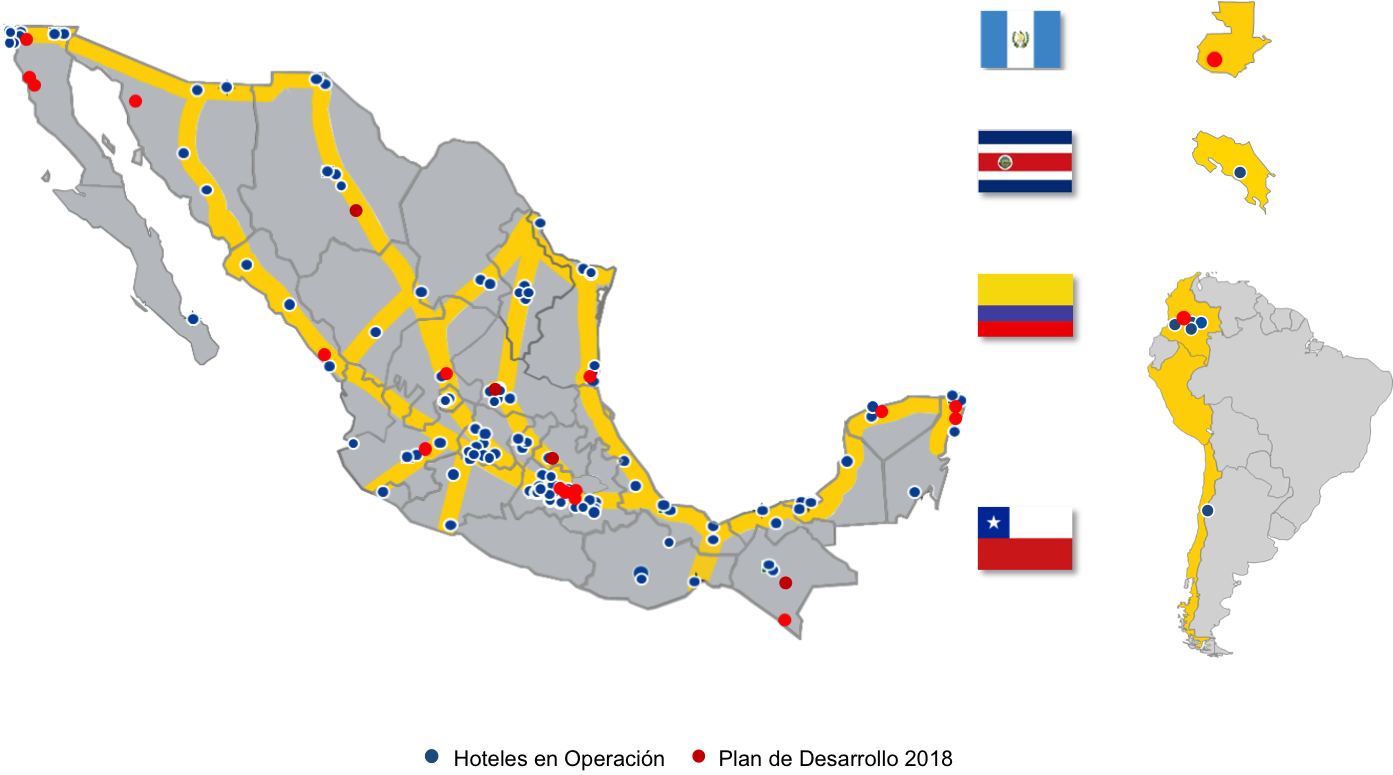
\includegraphics[width=\linewidth]{Imagenes/Ubicaciones.png}
  \caption{Plan de crecimiento}
  \label{fig:crecimiento}
\end{figure}
\section{Descripción del Problema}
\subsection{Gestión de las propiedades}
Hoteles CityExpress cuenta con un modelo de gestión comercial de sus propiedades ejecutado desde sus oficinas centrales ubicadas en la Ciudad de México. Este modelo de gestión se enfoca en optimizar la venta de los cuartos de las distintas propiedades, buscando siempre maximizar el ingreso obtenido por estas ventas.
Para poder entender mejor el modelo de gestión comercial debemos estudiar antes los canales distribución que utiliza para la venta de sus productos así como sus distintos segmentos de mercado. Posteriormente presentaremos las principales variables utilizadas para calificar el desempeño de las propiedades así como las acciones que puede tomar cada uno de los gerentes de las propiedades para poder cambiar el desempeño del hotel.
\paragraph{Canales de Venta}
~\\
CityExpress cuenta con un modelo de venta estandarizado para todas sus propiedades. Este modelo de venta contempla distintos canales de distribución que ayudan al grupo a poder incrementar la oferta de su producto llegando a distintos segmentos de mercado.
Es importante mencionar que cada uno de los canales de venta tienen un costo asociado, es decir, del ingreso que se perciba por cada cuarto vendido se debe tomar en cuenta el costo de cada canal para poder calcular la utilidad bruta de la venta, por eso es. importante conocer cómo opera cada uno de ellos.
Dentro de CityExpress existen dos tipos de canales de venta: \textbf{Canales de venta tradicionales} y \textbf{Canales de venta electrónicos}. Los canales de venta tradicionales, son aquellos en los cuales se requiere la intervención de un agente de ventas, los electrónicos permiten que el cliente final realice su reservación sin requerir la intervención del agente:
\paragraph{\textbf{Canales de venta tradicionales}}
\begin{itemize}[noitemsep]
\item Centro de Contacto (Call Center)
\item Hotel
\end{itemize}
\paragraph{\textbf{Canales de venta electrónicos}}
\begin{itemize}[noitemsep]
\item App (IOS y Android)
\item Portal Cliente Frecuente (City Premios)
\item Motor de reservaciones corporativas (CityAccess)
\item Motor de reservaciones (www.cityexpress.com.mx)
\item Agencias de viajes en línea (OTAs)
\end{itemize}
\paragraph{Segmentos de Mercado}
~\\
Los segmentos de mercado son un punto medular para poder entender el modelo de gestión en CityExpress ya que estos permiten al área comercial poder establecer una estrategia de venta en cada uno de los canales fijando precios en las distintas tarifas para poder maximizar la ocupación del hotel y el ingreso por cuartos vendidos. ~\\
Típicamente un hotel cuenta con un conjunto de tarifas las cuales son ofrecidas a diferentes segmentos de mercado en diferentes canales. Por ejemplo, un huésped que viaja por placer y reserva por la página web de CityExpress muy probablemente recibirá una tarifa distinta al huésped que viaja por negocios y reservó por el centro de contacto.
~\\
A continuación se presentan los distintos segmentos de mercado manejados por CityExpress:
~\\
\textbf{Negocios}
\begin{itemize}[noitemsep]
\item Directos
\item Convenios
\item Viajero Frecuente
\item Corporativo
\item Consorcios
\item Promociones
\item Otros
\end{itemize}
~\\
\textbf{Placer}
\begin{itemize}[noitemsep]
\item Directos
\item Fin de Semana
\item Otros
\item Promociones
\end{itemize}
~\\
\textbf{Mayoreo}
\begin{itemize}[noitemsep]
\item Agencias Minoristas
\item OTAs
\item Lineas Aéreas / Tripulaciones
\item Agencias Mayoristas
\item Otros
\end{itemize}
~\\
\textbf{Grupos}
\begin{itemize}[noitemsep]
\item Grupos, Ferias, Congresos y Convenciones
\item Sociales
\item Juntas
\item Deportes
\end{itemize}
~\\
\textbf{Otros}
\begin{itemize}[noitemsep]
\item Uso Casa
\item Cortesías
\item Intercambio
\item Empleados
\item Industria Turística
\item Otros
\end{itemize}
\paragraph{Tarifas}
~\\
Como se mencionó anteriormente, un hotel tiene un catálogo de 36 tarifas que puede ofrecer a los huéspedes. Cada tarifa va dirigida a un segmento de mercado y un canal en específico. Hay tarifas que pueden cambiar de precio hasta 3 veces al día y hay otras que al ser tarifas convenidas con otras empresas, permanecen estáticas la mayor parte del año.
Es responsabilidad de cada uno de los hoteles el revisar los distintos reportes expuestos en la organización en donde pueden encontrar: sus niveles de ocupación, ocupación de la competencia, tarifas promedio propias, tarifas promedio de la competencia, penetración de ocupación: $\frac{\% ocupacion\ propia}{ \% ocupacion\ de\ la\ competencia}$ y penetración de tarifa: $\frac{tarifa\ promedio\ propia}{tarifa\ promedio\ de\ la\ competencia}$ para decidir si deben hacer un incremento o decremento en los precios ofertados.
\paragraph{Variables estudiadas}
~\\
Dentro de CityExpress las decisiones de cambios de precios en las tarifas se toma analizando distintas variables. La mayoría de estas variables se alimentan de información propia del grupo hotelero aunque hay algunas que se obtienen de información de la competencia. A continuación se detallará cada una de las variables utilizadas durante la toma de estas decisiones:
\begin{itemize}[noitemsep]
\item \%Ocupacion
\item Tarifa Promedio
\item Tarifa Efectiva
\item Penetración de Ocupación
\item Penetración de Tarifa
\item Eventos por plaza
\item \%Ocupación de la competencia
\item Tarifa Promedio de la competencia
\item Tarifa Efectiva de la competencia
\end{itemize}
~\\
Derivado de las conclusiones del análisis de estas variables, los hoteles y el equipo de la oficina central pueden tomar alguna de las siguientes decisiones para alcanzar el objetivo deseado:
\begin{itemize}[noitemsep]
\item Subir precio de tarifa
\item Bajar precio de tarifa
\item Abrir un canal de venta
\item Cerrar un canal de venta
\item Promover la venta de un segmento específico mediante una promoción
\item Inhibir la venta de un segmento en específico cerrando disponibilidad de alguna tarifa
\end{itemize}
\subsection{Situación Actual}
~\\
Como se mencionó en el apartado anterior, hoy en día CityExpress gestiona su estrategia comercial desde las oficinas centrales delegando tareas clave a cada uno de los gerentes de las distintas propiedades, esto aunado al ambicioso plan de crecimiento de la cadena ha hecho que este modelo de gestión comercial se vuelva un proceso complicado de administrar y ejecutar de manera efectiva ya que se tienen las siguientes dependencias en el proceso:
\begin{itemize}[noitemsep]
\item Publicación de reportes diarios
\item Análisis de información publicada
\item Presentación de plan de acción de acuerdo al modelo de gestión
\item Aprobación del plan de acción por parte de la oficina central
\item Ejecución del plan de acción en los sistemas de control
\item Validación de resultados del plan de acción
\end{itemize}
\subsection{Propuesta de mejora al proceso}
~\\
Este proyecto tiene como objetivo mejorar el proceso de gestión de hoteles en CityExpress mediante la construcción de un sitio en donde se integre toda la información que hoy en día se expone en distintos reportes dentro de la empresa y además cuente con un modelo que permita pronosticar el $\%\ de\ ocupacion$ de cada una de las propiedades y a su vez haga una recomendación del precio para la tarifa que se ofrece al público en general que ayude a maximizar el ingreso por venta de cuartos dentro de la propiedad.
Con esta herramienta se espera que el modelo de gestión comercial se automatice y la ejecución del plan de acción se realice de manera más ágil.
\section{Metodología Propuesta}
\subsection{Plan de implementación}
~\\
A continuación se presentan los pasos que se siguieron para la implementación de este nuevo sistema de gestión:
\begin{description}
\item [$\bullet$ Entendimiento del negocio:]  Antes de construir una herramienta / producto de datos se dedicó un tiempo a conocer los procesos operativos de la cadena hotelera.
\item [$\bullet$ Entendimiento del sistema de gestión comercial:] Para que el producto final agregue verdadero valor a la empresa se debió comprender el tramo de control de cada puesto operativo destinado a hacer uso de esta herramienta, es decir, se identificaron las acciones que cada usuario puede ejecutar en los distintos sistemas para alcanzar sus objetivos comerciales.
\item [$\bullet$ Identificación de posibles fuentes de datos:] Una vez comprendidos los procesos operativos y de toma de decisiones, se identificaron los sistemas que proveen la información que ayuda al personal de CityExpress durante la toma de decisiones.
\item [$\bullet$ Análisis exploratorio de datos:] Una vez identificadas las fuentes de datos, se ejecutó un análisis exploratorio de datos con el fin de poder conocer los datos con que se trabajaron para posteriormente fijar un alcance para el producto final.
\item [$\bullet$ Modelo de predicción de ocupación y sugerencia de precios:] Una vez perfilados los datos y con un EDA concluido se realizó un esfuerzo para construir un modelo que fuera capaz de pronosticar el $\%\ de\ ocupacion$ y que sugiriera el $precio\ publico$ óptimo de cada una de las propiedades.
\item [$\bullet$ Construcción de prototipo de producto de datos:] Se definió la arquitectura final del producto de datos y se construyó un prototipo totalmente funcional que apoya la toma de decisiones de los participantes del proceso de gestión comercial.
\end{description}
\subsection{Fuentes de datos}
~\\
Una vez hecho el análisis de negocio y conociendo la operación de CityExpress, detectamos que las fuentes principales para la construcción del producto de datos son las siguientes:
\begin{itemize}
\item \textbf{Central de Reservaciones}: Módulo encargado de realizar las reservaciones de cuartos en las distintas propiedades. De este sistema obtuvimos el comportamiento histórico de cada una de las propiedades, es decir, cuantas habitaciones fueron reservadas, en qué momento y con qué tarifa.
\item \textbf{Property Management System (PMS)}: Módulo encargado de gestionar las propiedades. Aquí se pueden consultar las habitaciones ocupadas, disponibles y fuera de servicio, así como las llegadas y salidas del día. De este sistema obtuvimos las reservaciones en libros (bookings) o llegadas pendientes, esta información es crucial para poder conocer en la demanda real de cada una de las propiedades en el tiempo.
\item \textbf{Market Share}: Sistema encargado de recopilar la información de la competencia. Las variables recopiladas son Tarifa Promedio, Habitaciones Disponibles, Habitaciones ocupadas, entre otras. 
\item \textbf{Tarifas de la competencia}: Consulta de las tarifas disponibles en las agencias de viajes en línea para la competencia.
\end{itemize}
\subsection{Análisis Exploratorio de Datos}
A continuación se mostrará a detalle análisis exploratorio realizado al dataset inicial. Este data set comprendía información de 5 hoteles y el objetivo de este era brindar un apoyo a la comprensión de los datos para poder establecer una metodología de trabajo al momento de crear un modelo de predicción de demanda para cada una de las propiedades. Para fines de este trabajo detallaremos el "EDA" utilizando datos de una sola propiedad: "CEXXX".
\paragraph{Descripción del DataSet} ~\\
Durante la construcción del modelo se hizo uso de tres datasets principalmente. El primero de ellos llamado "histórico\_ocupación" fue obtenido del sistema de gestión de propiedades \textbf{(PMS)} y contiene la información del desempeño histórico de las propiedades. A continuación se presenta un resumen del data set en cuestión.

\begin{knitrout}
\definecolor{shadecolor}{rgb}{0.969, 0.969, 0.969}\color{fgcolor}\begin{kframe}
\begin{verbatim}
##    rsrv_code        date_create                 
##  Min.   :6265739   Min.   :2016-07-20 18:31:59  
##  1st Qu.:7499788   1st Qu.:2017-03-27 10:10:09  
##  Median :7999769   Median :2017-06-30 12:12:57  
##  Mean   :8007253   Mean   :2017-06-27 13:38:02  
##  3rd Qu.:8505582   3rd Qu.:2017-09-27 13:22:36  
##  Max.   :9053354   Max.   :2018-01-01 03:08:21  
##     date_in                   
##  Min.   :2017-01-01 00:00:00  
##  1st Qu.:2017-04-04 00:00:00  
##  Median :2017-07-06 00:00:00  
##  Mean   :2017-07-06 02:18:17  
##  3rd Qu.:2017-10-08 00:00:00  
##  Max.   :2017-12-31 00:00:00  
##     date_out                       nights 
##  Min.   :2017-01-02 00:00:00   Min.   :1  
##  1st Qu.:2017-04-05 00:00:00   1st Qu.:1  
##  Median :2017-07-07 00:00:00   Median :1  
##  Mean   :2017-07-07 02:18:17   Mean   :1  
##  3rd Qu.:2017-10-09 00:00:00   3rd Qu.:1  
##  Max.   :2018-01-01 00:00:00   Max.   :1  
##   prop_code           mkt_sgm            Dia_Sem         
##  Length:44391       Length:44391       Length:44391      
##  Class :character   Class :character   Class :character  
##  Mode  :character   Mode  :character   Mode  :character  
##                                                          
##                                                          
##                                                          
##   rate_code            bucket             Ingresos   
##  Length:44391       Length:44391       Min.   :   0  
##  Class :character   Class :character   1st Qu.:1200  
##  Mode  :character   Mode  :character   Median :1462  
##                                        Mean   :1449  
##                                        3rd Qu.:1658  
##                                        Max.   :3900  
##    rsrv_src          rsrv_type          room_type        
##  Length:44391       Length:44391       Length:44391      
##  Class :character   Class :character   Class :character  
##  Mode  :character   Mode  :character   Mode  :character  
##                                                          
##                                                          
##                                                          
##       pax       
##  Min.   :0.000  
##  1st Qu.:1.000  
##  Median :1.000  
##  Mean   :1.271  
##  3rd Qu.:1.000  
##  Max.   :5.000
\end{verbatim}
\end{kframe}
\end{knitrout}
~\\
A continuación se presenta el diccionario de datos para el data set presentado:
\begin{itemize}[noitemsep]
\item rsrv\_code: Código de confirmación de reserva
\item date\_create: Fecha de creación de la reserva
\item date\_in:Fecha de entrada al hotel
\item date\_out: Fecha de salida del hotel
\item nights: Número de noches en el hotel
\item prop\_code: Código de Hotel
\item mkt\_sgm: Segmento de Mercado
\item Dia\_Sem: Dia de la semana para la fecha de entrada al hotel
\item rate\_code: Código de tarifa
\item bucket: Nivel de tarifa
\item Ingresos: Ingresos obtenidos por la reservación
\item rsrv\_src: Canal de la reservación
\item rsrv\_type: Tipo de reservación
\item room\_type: Tipo de habitación
\item PAX: Personas amparadas por la reservación
\end{itemize}
~\\
Revisando el resumen de este data set es importante resaltar que los datos fueron trabajados previamente para presentarse de manera desagregada, es decir, si una reserva ampara una estancia de 5 noches tendremos un registro por cada noche de la estancia, por ejemplo:
~\\
\begin{knitrout}
\definecolor{shadecolor}{rgb}{0.969, 0.969, 0.969}\color{fgcolor}\begin{table}[H]
\centering\rowcolors{2}{gray!6}{white}

\begin{tabular}{r|l|l|l|r|l}
\hiderowcolors
\hline
rsrv\_code & date\_create & date\_in & date\_out & nights & room\_type\\
\hline
\showrowcolors
6265739 & 2016-07-20 18:31:59 & 2017-04-07 & 2017-04-08 & 1 & NSK\\
\hline
6265739 & 2016-07-20 18:31:59 & 2017-04-08 & 2017-04-09 & 1 & NSK\\
\hline
6265739 & 2016-07-20 18:31:59 & 2017-04-09 & 2017-04-10 & 1 & NSK\\
\hline
6265739 & 2016-07-20 18:31:59 & 2017-04-10 & 2017-04-11 & 1 & NSK\\
\hline
6265739 & 2016-07-20 18:31:59 & 2017-04-11 & 2017-04-12 & 1 & NSK\\
\hline
6265739 & 2016-07-20 18:31:59 & 2017-04-12 & 2017-04-13 & 1 & NSK\\
\hline
\end{tabular}
\rowcolors{2}{white}{white}
\end{table}


\end{knitrout}
Como podemos observar el numero de reservación es el mismo en los 6 registros, lo mismo ocurre con la fecha de creación, las noches, y el tipo de habitación, sin embargo, la fecha de entrada y la fecha de salida va cambiando en cada registro. En algunos casos es más fácil trabajar con los registros desagregados, sin embargo hay casos en dónde necesitaremos agrupar la información.

\paragraph{Ocupación} ~\\
De las primeras preguntas que se vienen a la mente al momento de analizar la información de esta propiedad es ¿Qué nivel de ocupación tiene este hotel a lo largo del tiempo? Para contestar esta pregunta, se generáron las siguientes gráficas:
~\\
\begin{knitrout}
\definecolor{shadecolor}{rgb}{0.969, 0.969, 0.969}\color{fgcolor}
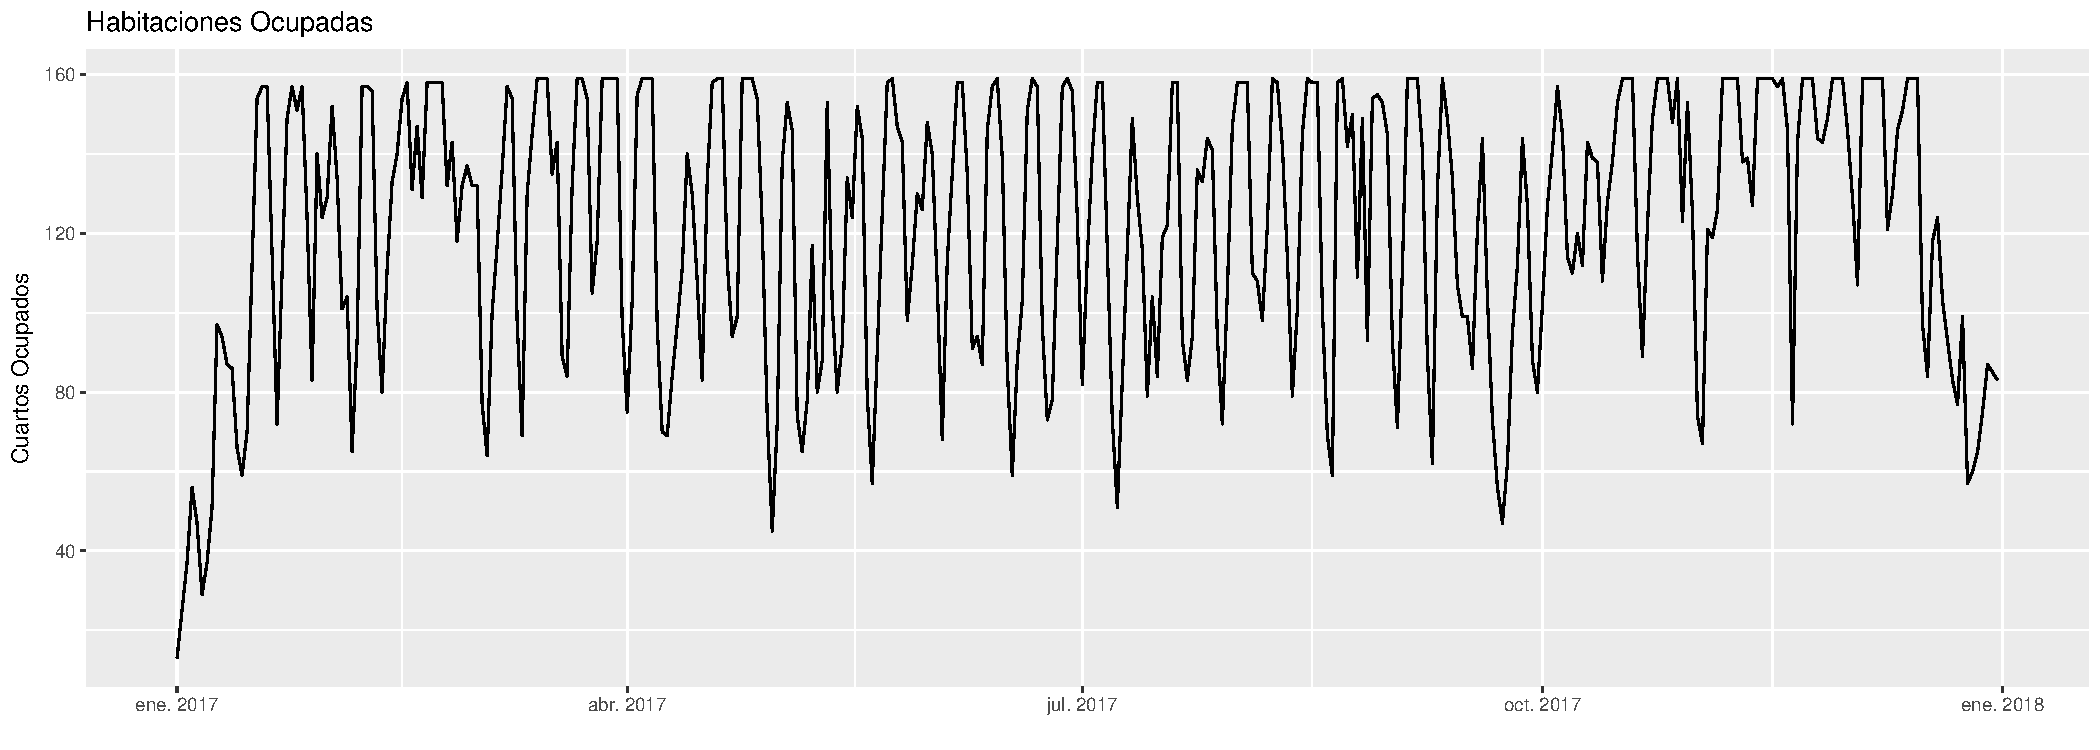
\includegraphics[width=\maxwidth]{figures/HabitacionesOcupadas-1} 

\end{knitrout}
~\\
\begin{knitrout}
\definecolor{shadecolor}{rgb}{0.969, 0.969, 0.969}\color{fgcolor}
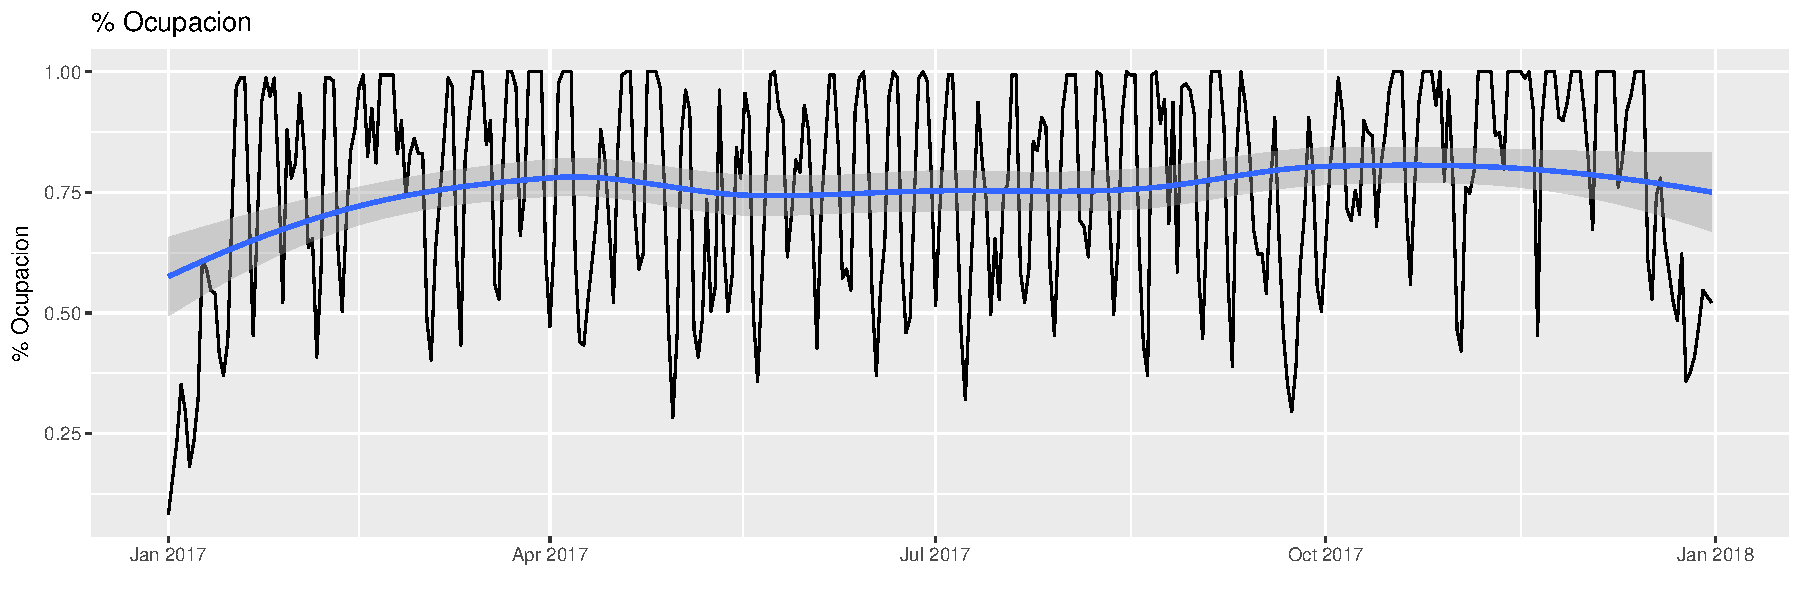
\includegraphics[width=\maxwidth]{figures/Ocupacion-1} 

\end{knitrout}
~\\
Como podemos observar esta propiedad tiene niveles de ocupación alrededor del 75\% llegando en repetidas ocasiones al 100\% de ocupación. Las caídas en los níveles de ocupación se deben a los fines de semana. A continuación presentamos una gráfica que nos ayudará a sustentar esta conclusión.
~\\
\begin{knitrout}
\definecolor{shadecolor}{rgb}{0.969, 0.969, 0.969}\color{fgcolor}
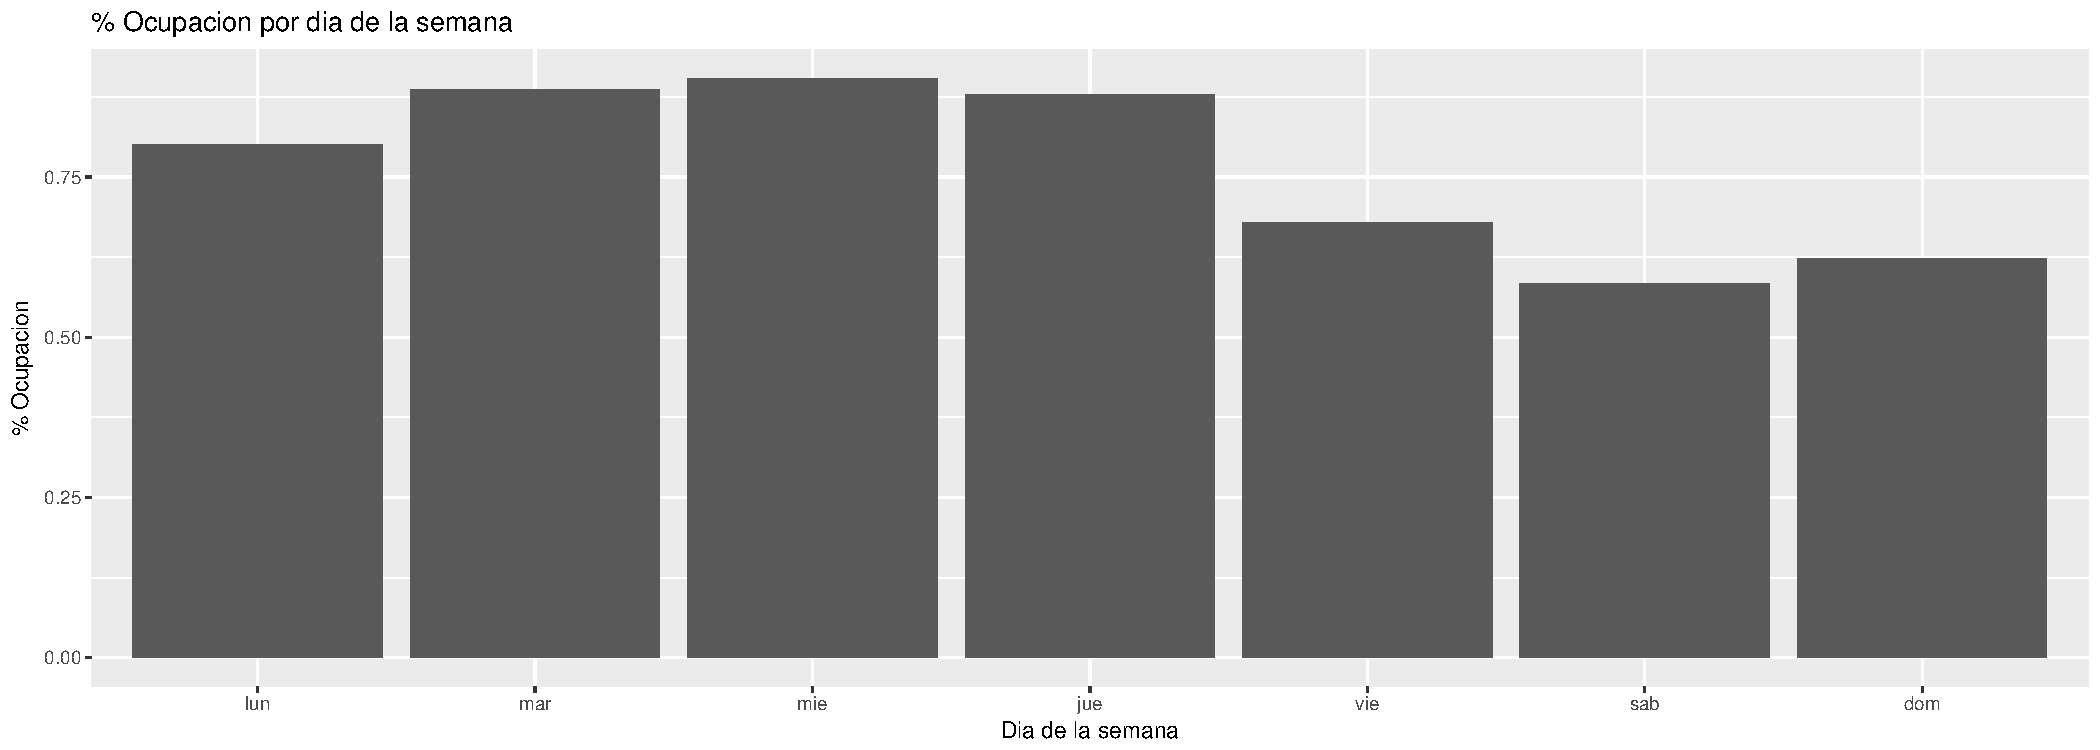
\includegraphics[width=\maxwidth]{figures/Ocupacion_Dia_Semana-1} 

\end{knitrout}
\paragraph{Pickup} ~\\
Al realizar este tipo de análisis resulta interesante estudiar el tiempo de antelación con el cual el cliente reserva un cuarto, a esto se le llama curva de pickup. Para poder graficar esta curva necesitaremos agrupar los datos por numero de reservación obteniendo la mínima fecha de entrada y la máxima fecha de salida para cada una de ellas. Una vez trabajados los datos podremos calcular la antelación obteniendo la diferencia entre la fecha de entrada y la fecha de creación en días.
~\\
\begin{knitrout}
\definecolor{shadecolor}{rgb}{0.969, 0.969, 0.969}\color{fgcolor}
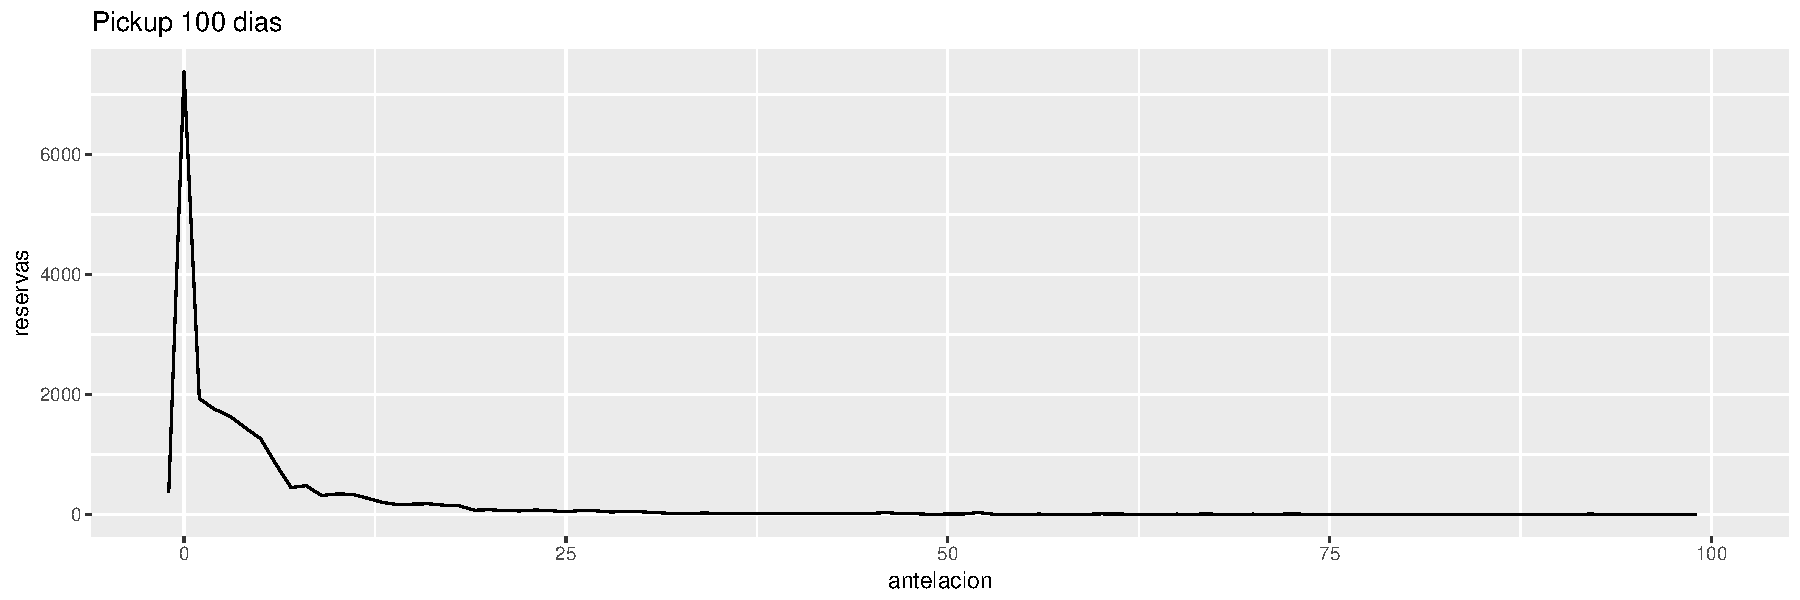
\includegraphics[width=\maxwidth]{figures/pickup-1} 

\end{knitrout}
~\\
\begin{knitrout}
\definecolor{shadecolor}{rgb}{0.969, 0.969, 0.969}\color{fgcolor}
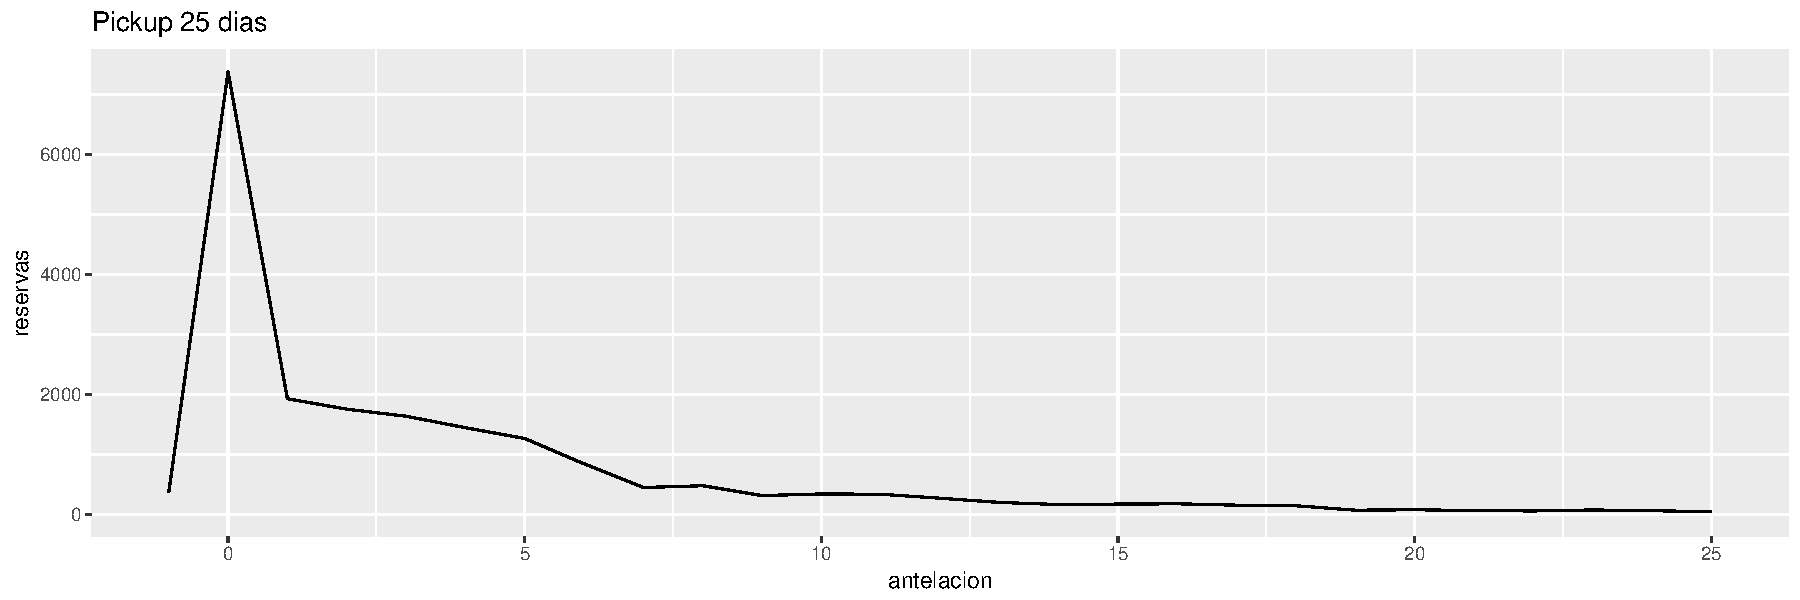
\includegraphics[width=\maxwidth]{figures/pickupzoom-1} 

\end{knitrout}
\paragraph{Pickup por Canal de Venta} ~\\
Como podemos observar en la gráfica "Pickup 25 días" el mayor número de reservaciones en esta propiedad ocurre 5 días antes de que el huésped llegue al hotel. Con esto podemos concluír que los clientes que visitan esta propiedad planean su estancia con a lo más 5 días de antelación. 
Resulta interesante ampliar este análisis para cada uno de los canales de reservación disponibles.
~\\
\begin{knitrout}
\definecolor{shadecolor}{rgb}{0.969, 0.969, 0.969}\color{fgcolor}
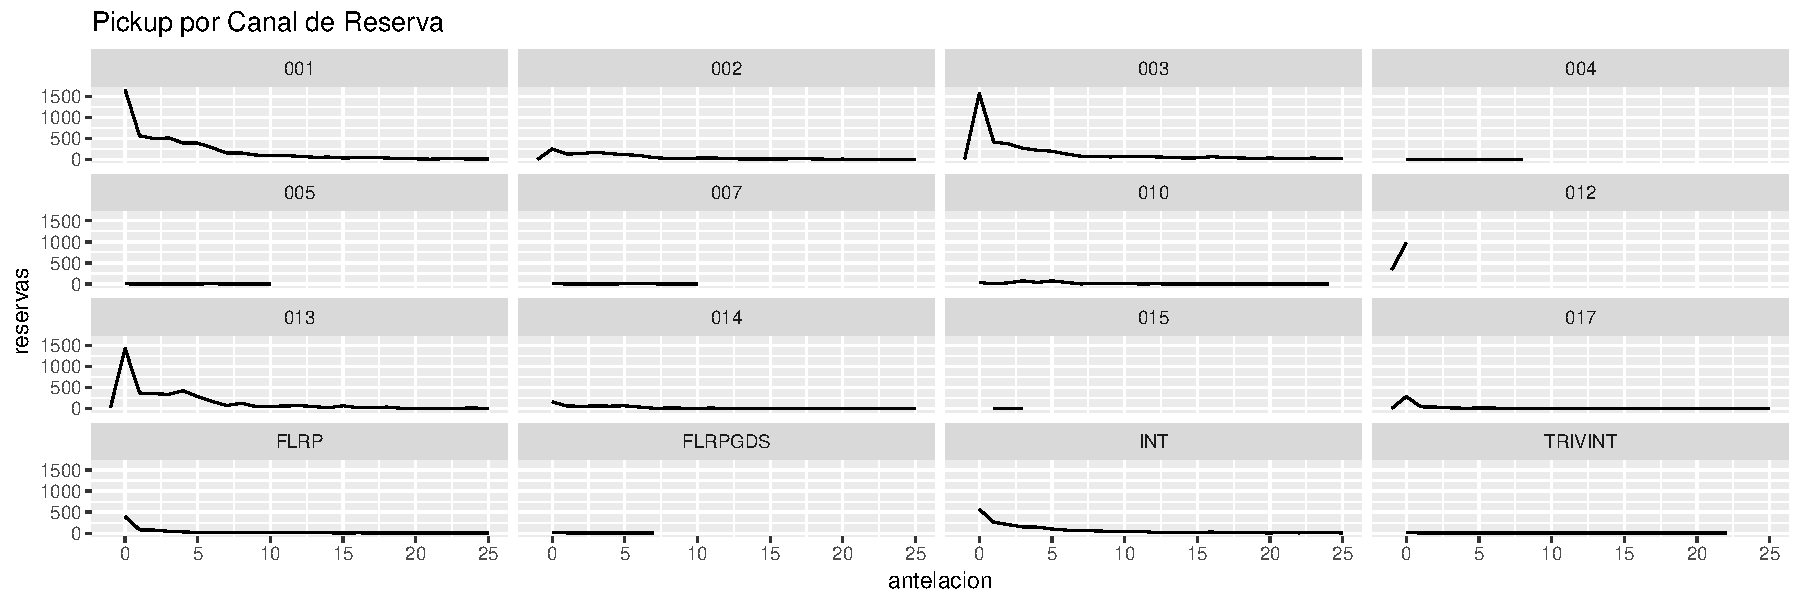
\includegraphics[width=\maxwidth]{figures/pickupsrc-1} 

\end{knitrout}
~\\
Podemos notar que para este hotel en particular el pickup es similar (alrededor de 5 días de antelación) en los canales que producen ventas de cuartos, sin embargo resulta interesante observar que no todos los canales tienen una producción significativa en esta propiedad ya que el grueso de las ventas se concentra en los siguientes canales:
\begin{itemize}[noitemsep]
\item Contact Center
\item Hotel
\item Ota's
\item Internet (Website)
\item GDS's
\end{itemize}
\paragraph{Canales de Venta} ~\\
\begin{knitrout}
\definecolor{shadecolor}{rgb}{0.969, 0.969, 0.969}\color{fgcolor}
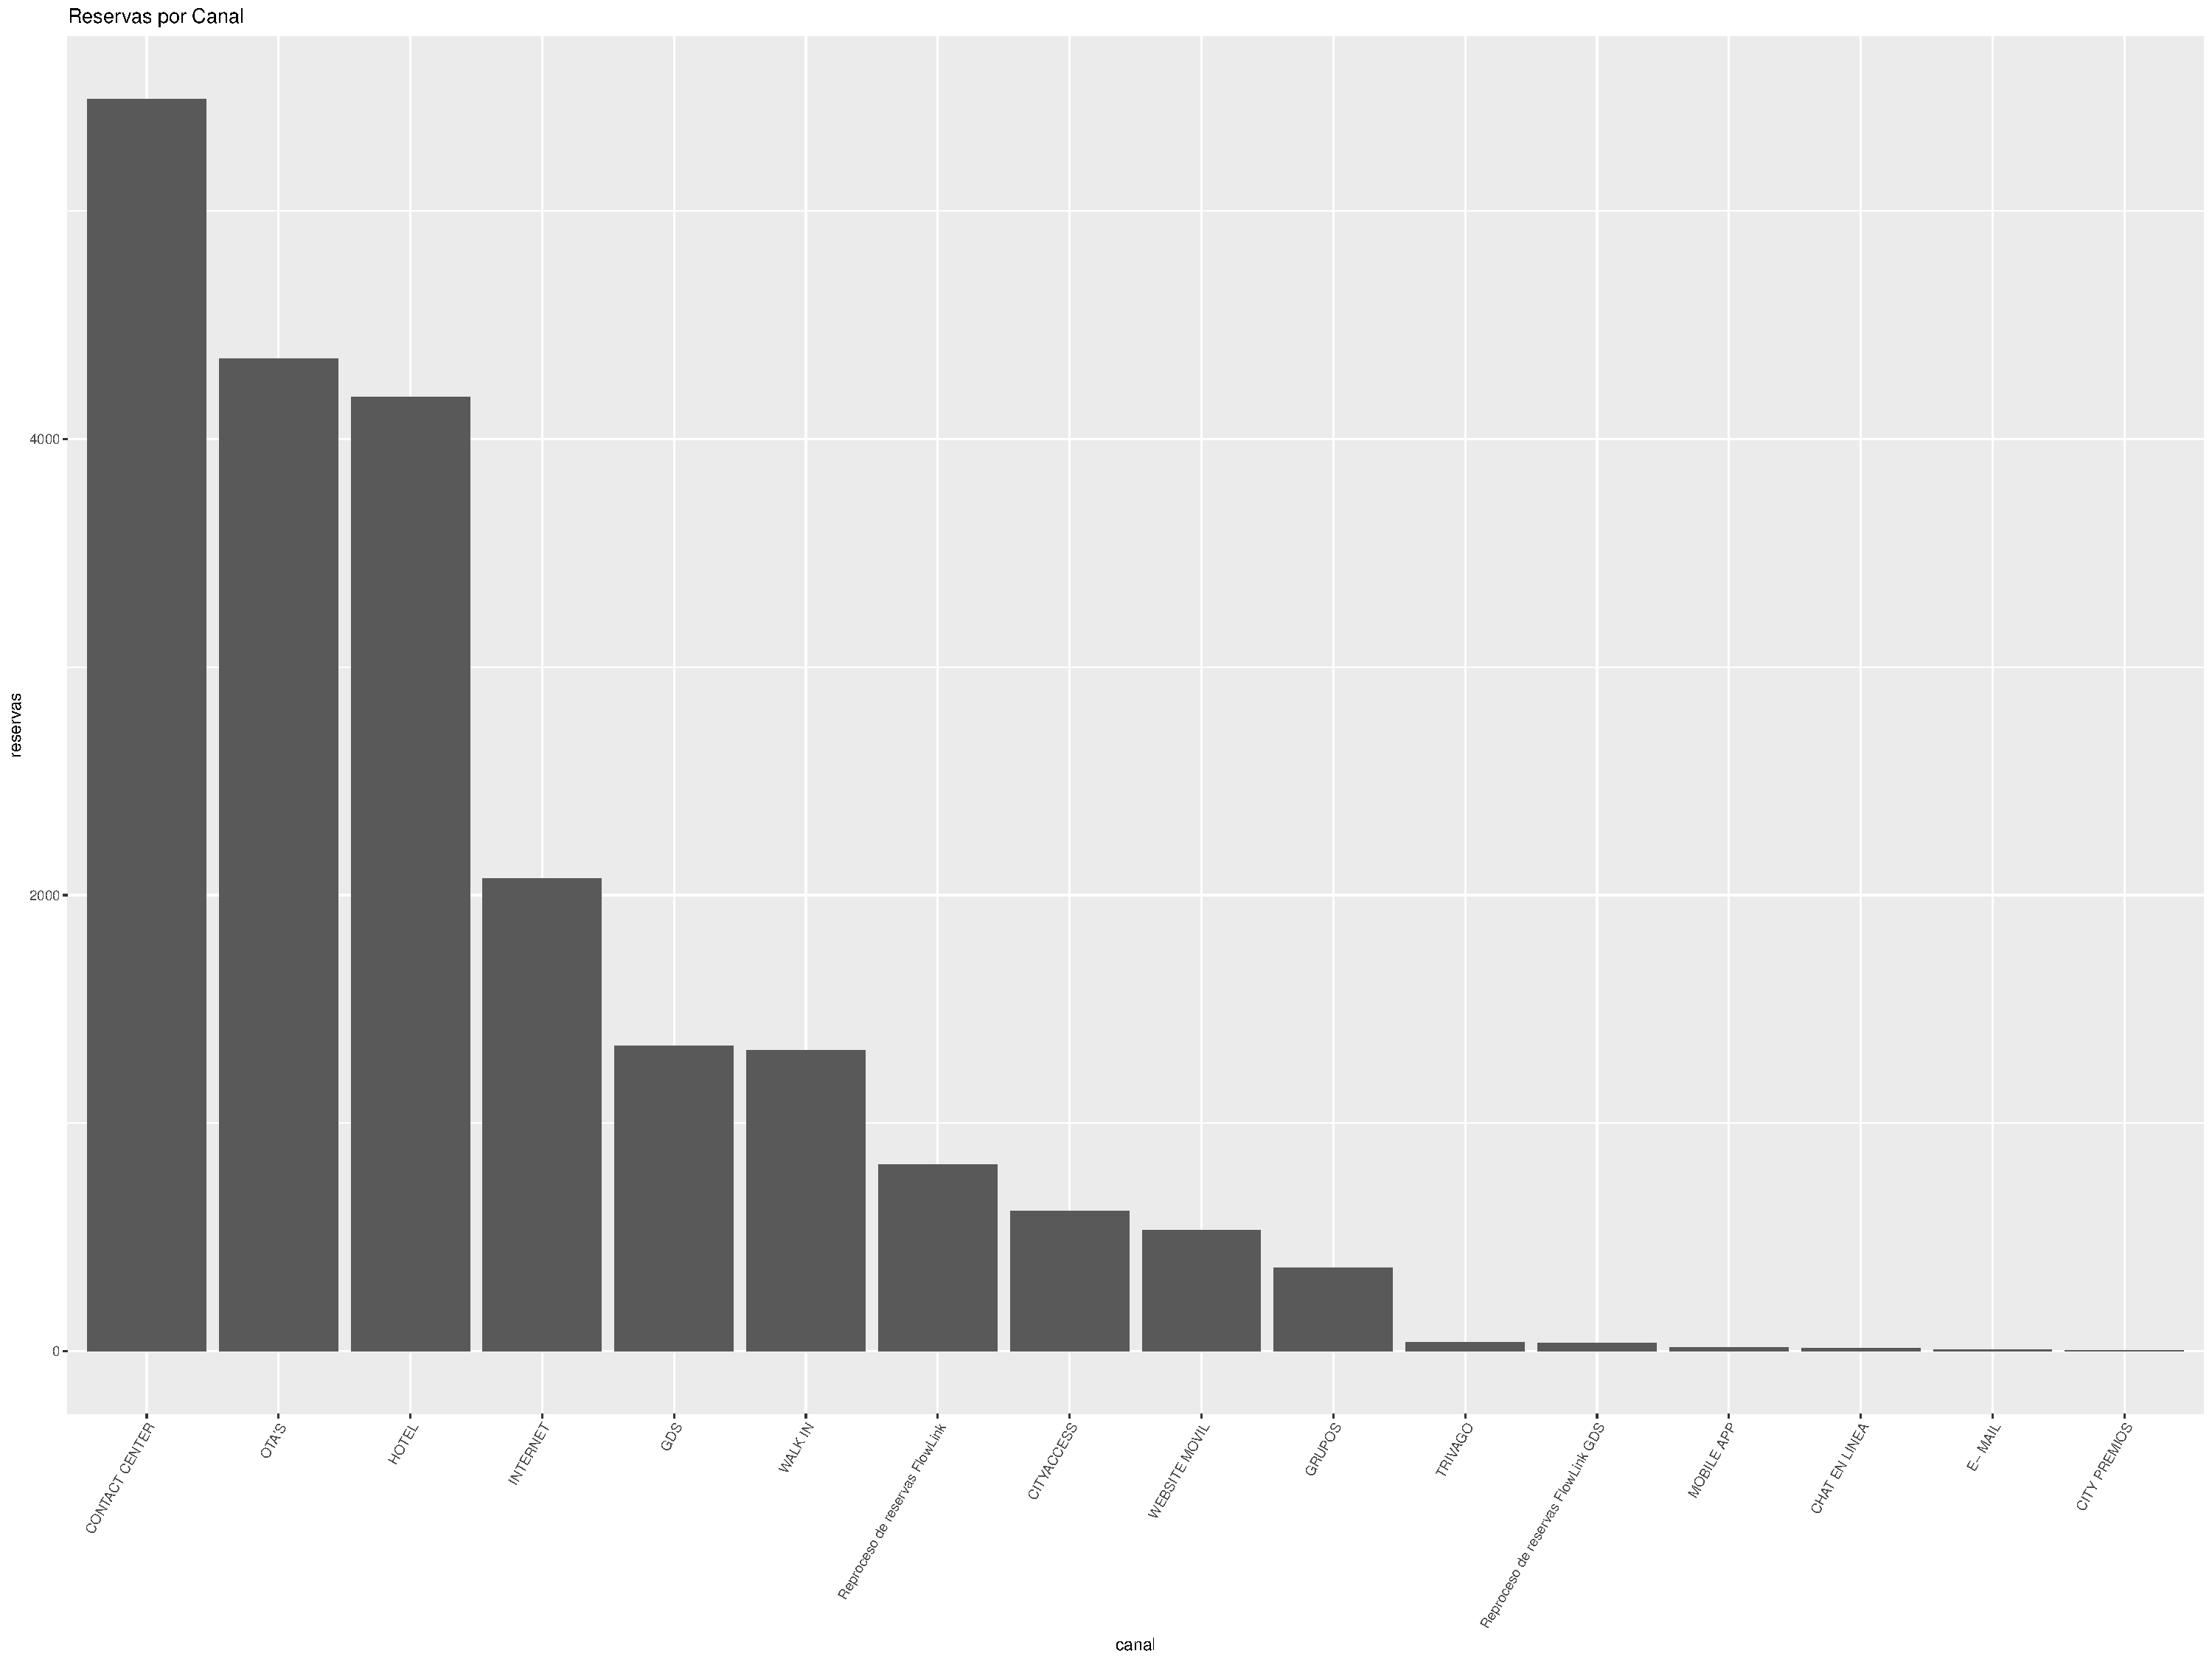
\includegraphics[width=\maxwidth]{figures/reservacionesxcanal-1} 

\end{knitrout}
~\\
Por último estudiaremos cómo se comporta cada uno de los canales a lo largo del día, esto para poder encontrar un patrón en el uso de cada uno de los canales.
~\\
\begin{knitrout}
\definecolor{shadecolor}{rgb}{0.969, 0.969, 0.969}\color{fgcolor}
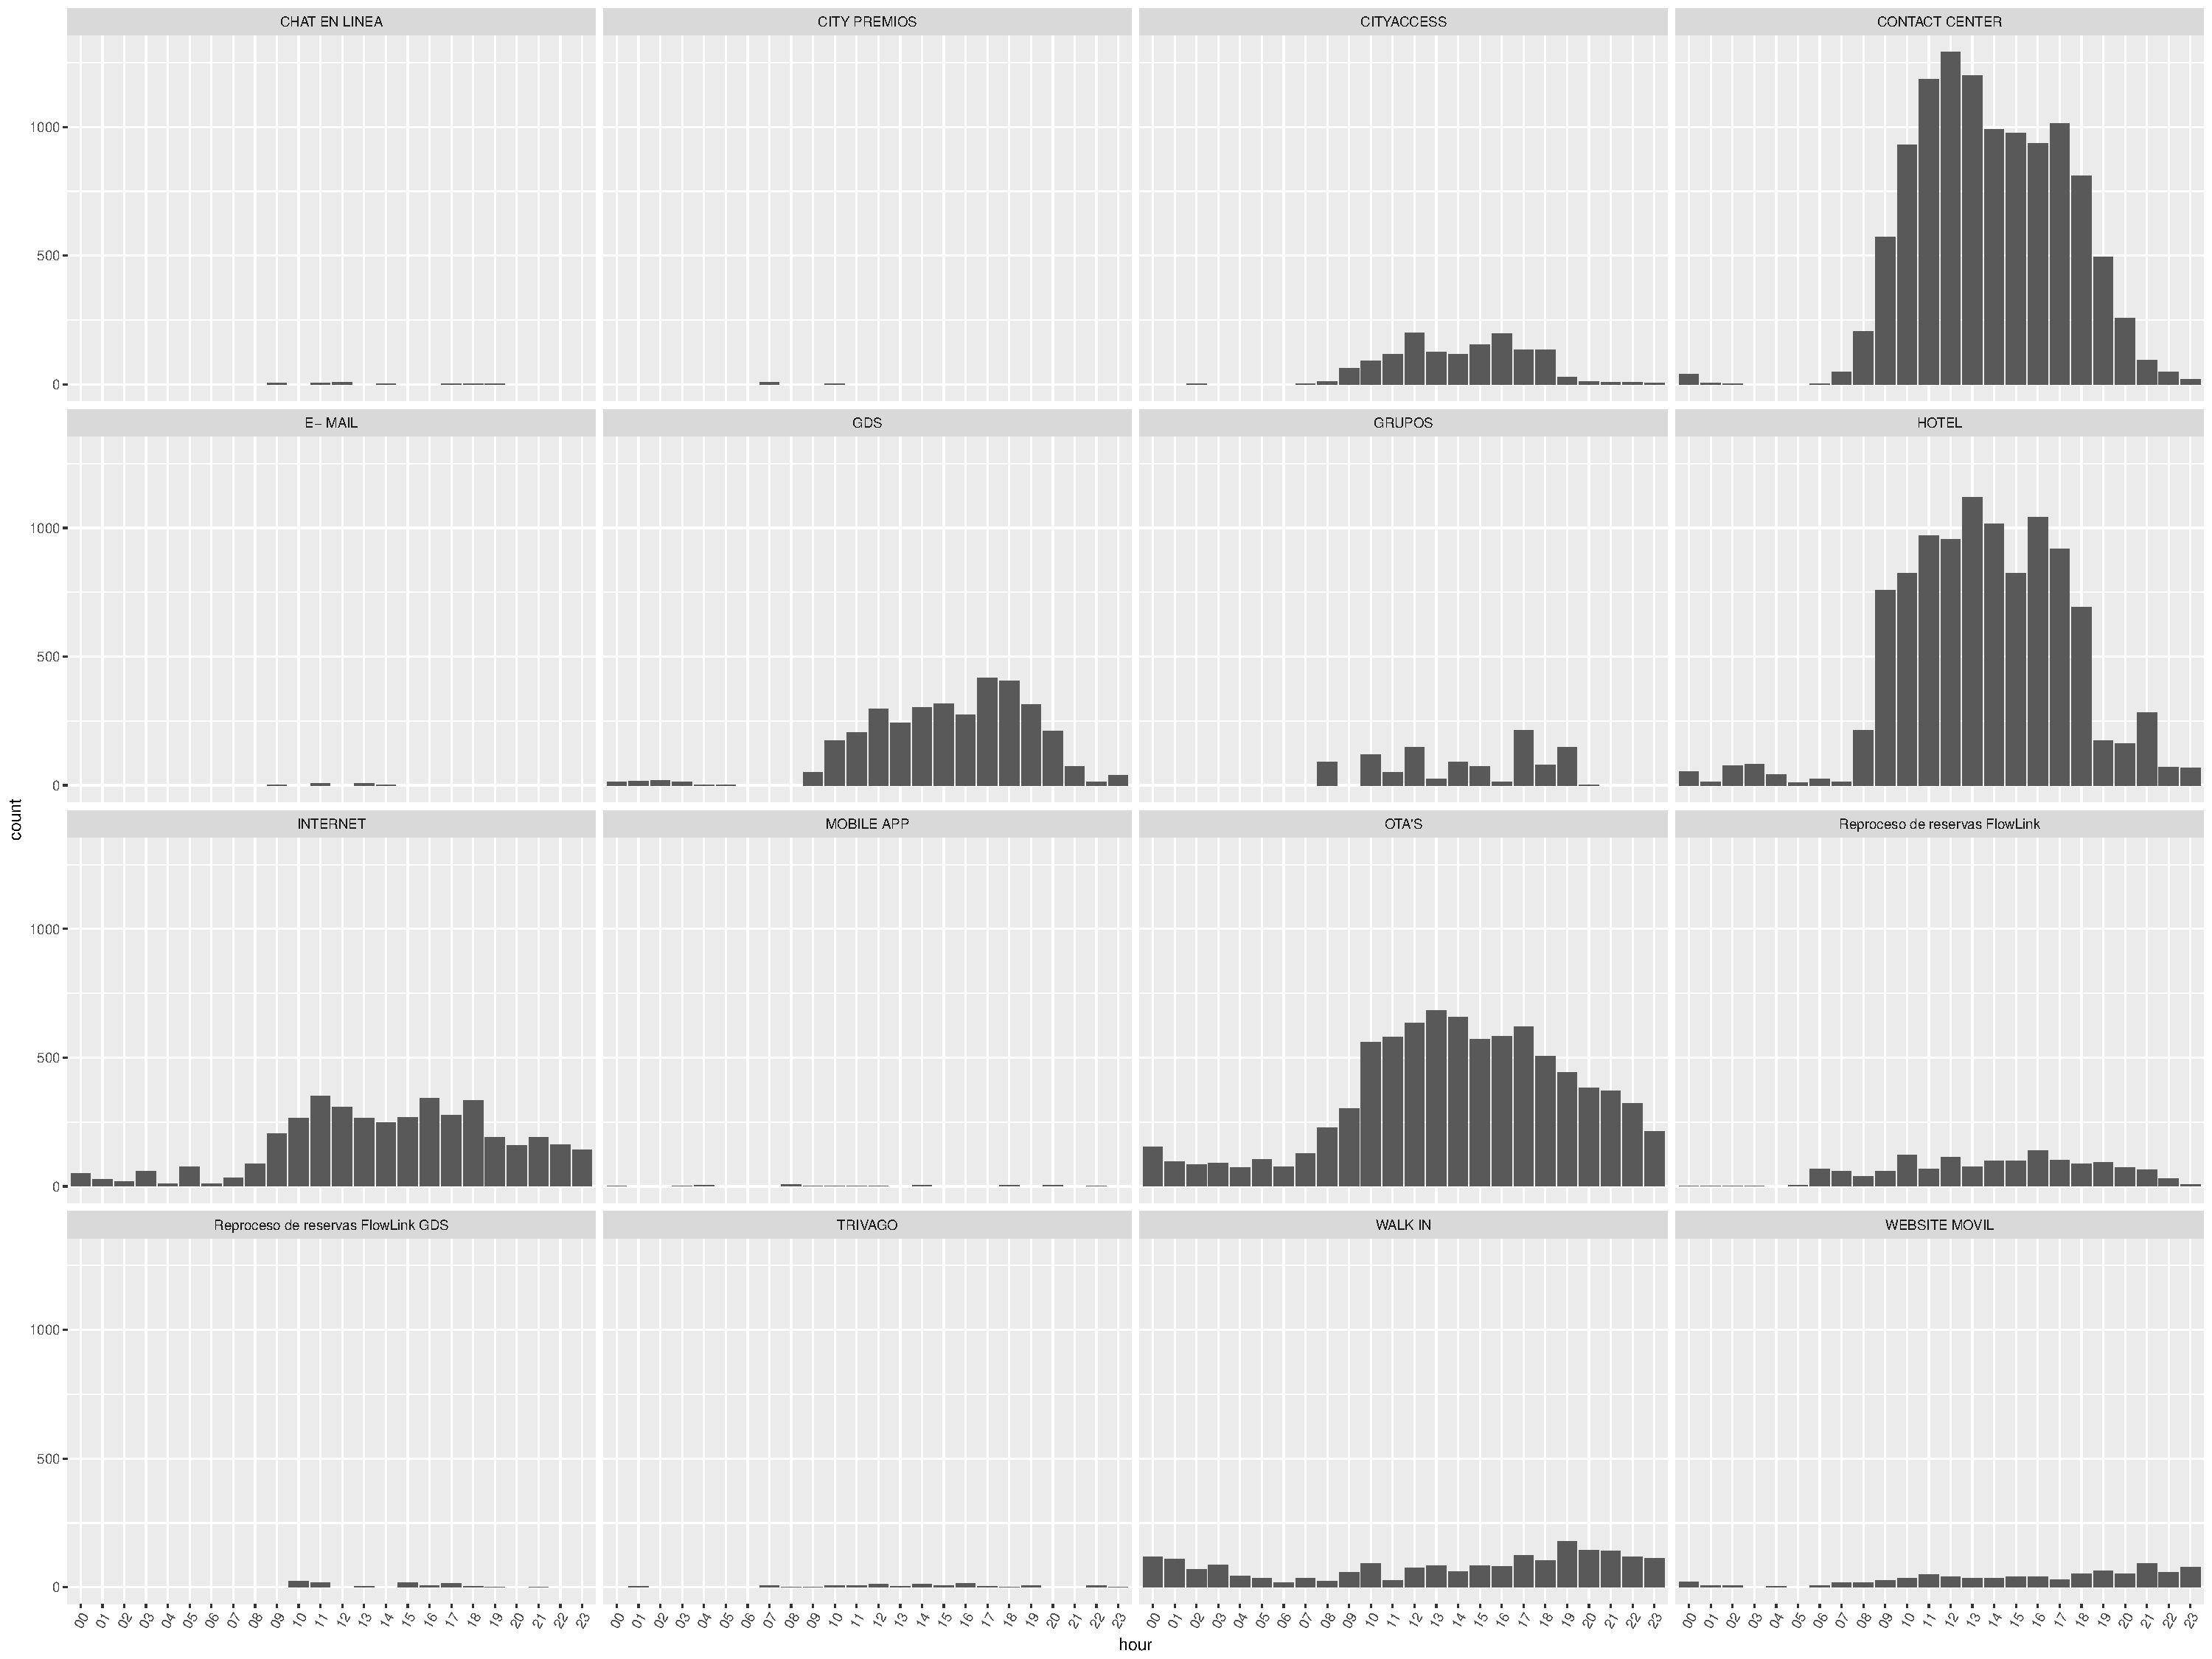
\includegraphics[width=\maxwidth]{figures/CorrelacionHoraCanal-1} 

\end{knitrout}
~\\
Con la gráfica anterior podemos corroborar los canales de venta más activos para este hotel y podemos concluír también que las horario en el que esta propiedad genera más reservaciones es de 9:00 am a 9:00 pm, con excepción del canal "walk in" el cuál tiene una distribución uniforme en las reservas generadas a lo largo del día.
\paragraph{Segmentos de Mercado} ~\\
Como se mencionó anteriormente, City Express implementa una segmentación de mercado en cada una de las reservaciones que genera, esto nos permitirá analizar el perfil del huésped que visita cada una de las propiedades. A continuación presentaremos un análisis partícular para una de las propiedades.
A continuación se presentan los segmentos de mercado y las reservaciones que produjeron durante un periodo de tiempo:
~\\
\begin{knitrout}
\definecolor{shadecolor}{rgb}{0.969, 0.969, 0.969}\color{fgcolor}
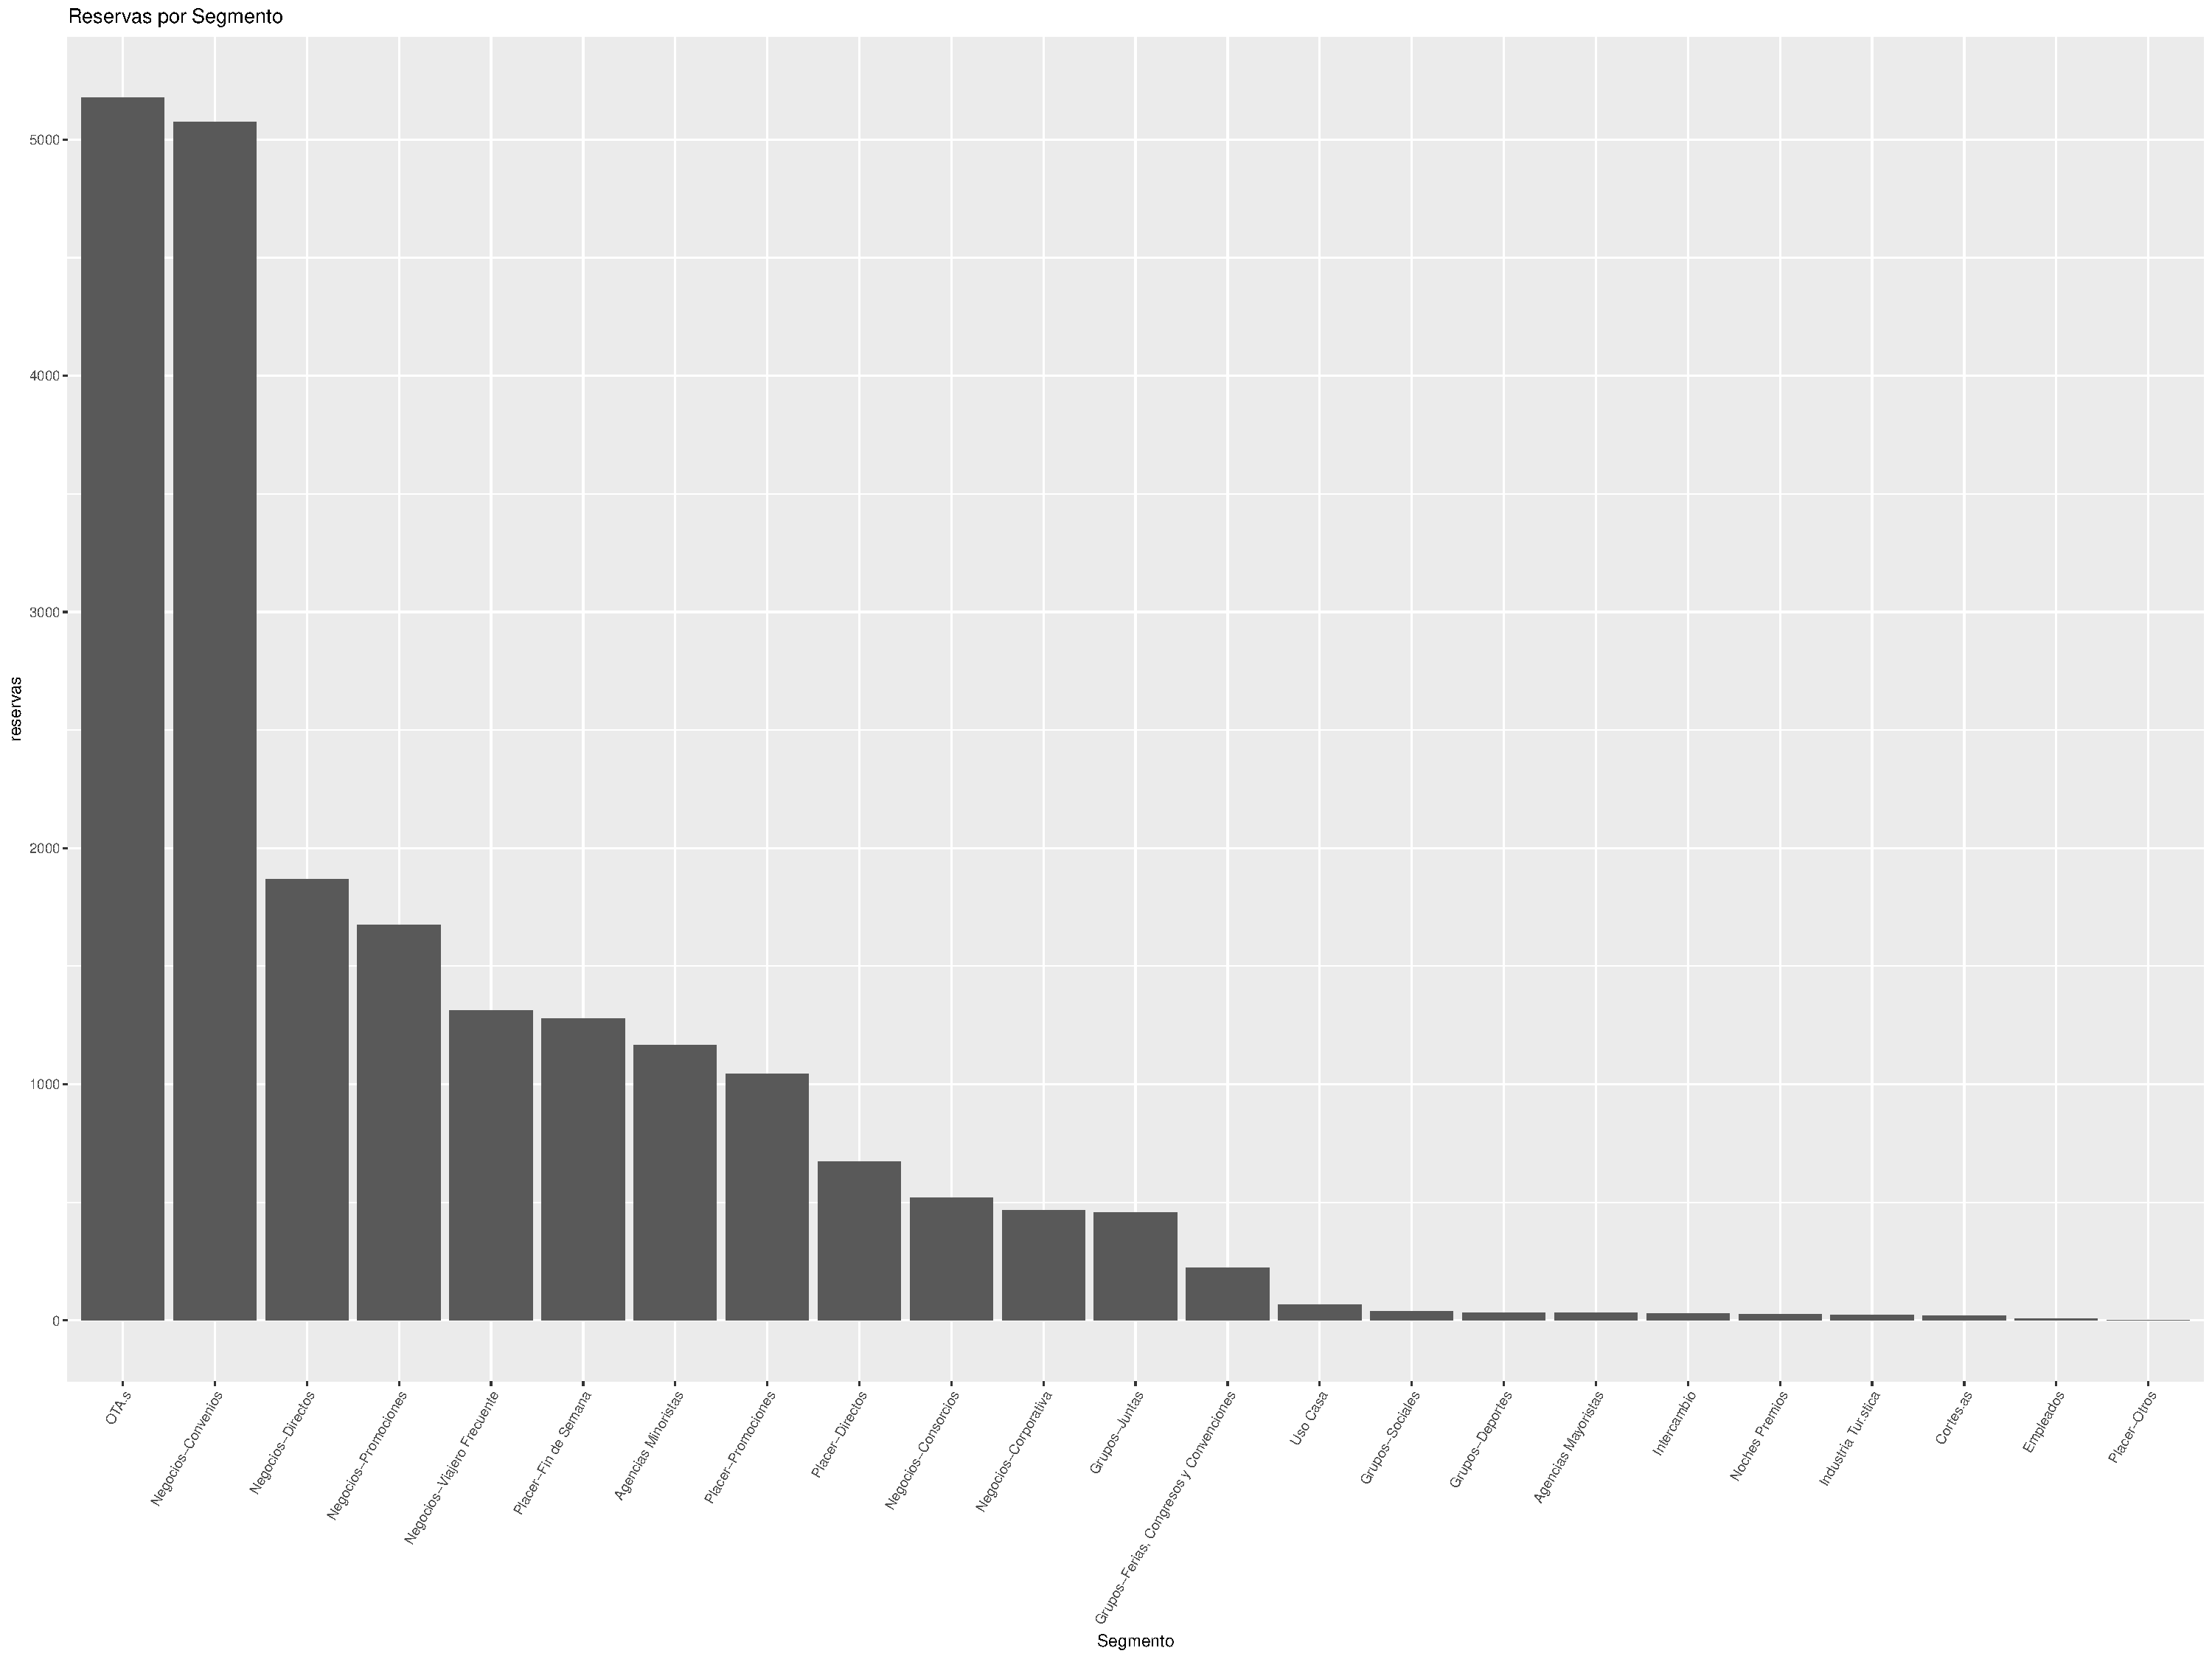
\includegraphics[width=\maxwidth]{figures/SegmentosMercado-1} 

\end{knitrout}
~\\
Derivado de este analisis podemos observar lo siguiente:
Los segmentos que mas reservan son:
\begin{itemize}[noitemsep]
\item OTA's (Agencias de Viaje en línea)
\item Negocios-Convenios (Empresas con tarifa convenio)
\item Negocios-Directos (Viajeros de negocios sin tarifas convenio)
\item Negocios-Promociones (Viajeros de negocios con cupones promocionales)
\end{itemize}
Podemos decir que el perfil del huésped que visita esta propiedad es el viajero de negocios que visita oficinas corporativas cercanas a la ubicación del hotel durante la semana laboral (Lunes - Viernes).
\paragraph{Producción de Cuartos por Segmentos} ~\\
Contrastaremos la gráfica anterior contra la producción de cuartos vendidos por cada uno de los segmentos para poder tener una ídea de cuantos cuartos vende cada segmento en cada una de las reservaciones generadas.
~\\
\begin{knitrout}
\definecolor{shadecolor}{rgb}{0.969, 0.969, 0.969}\color{fgcolor}
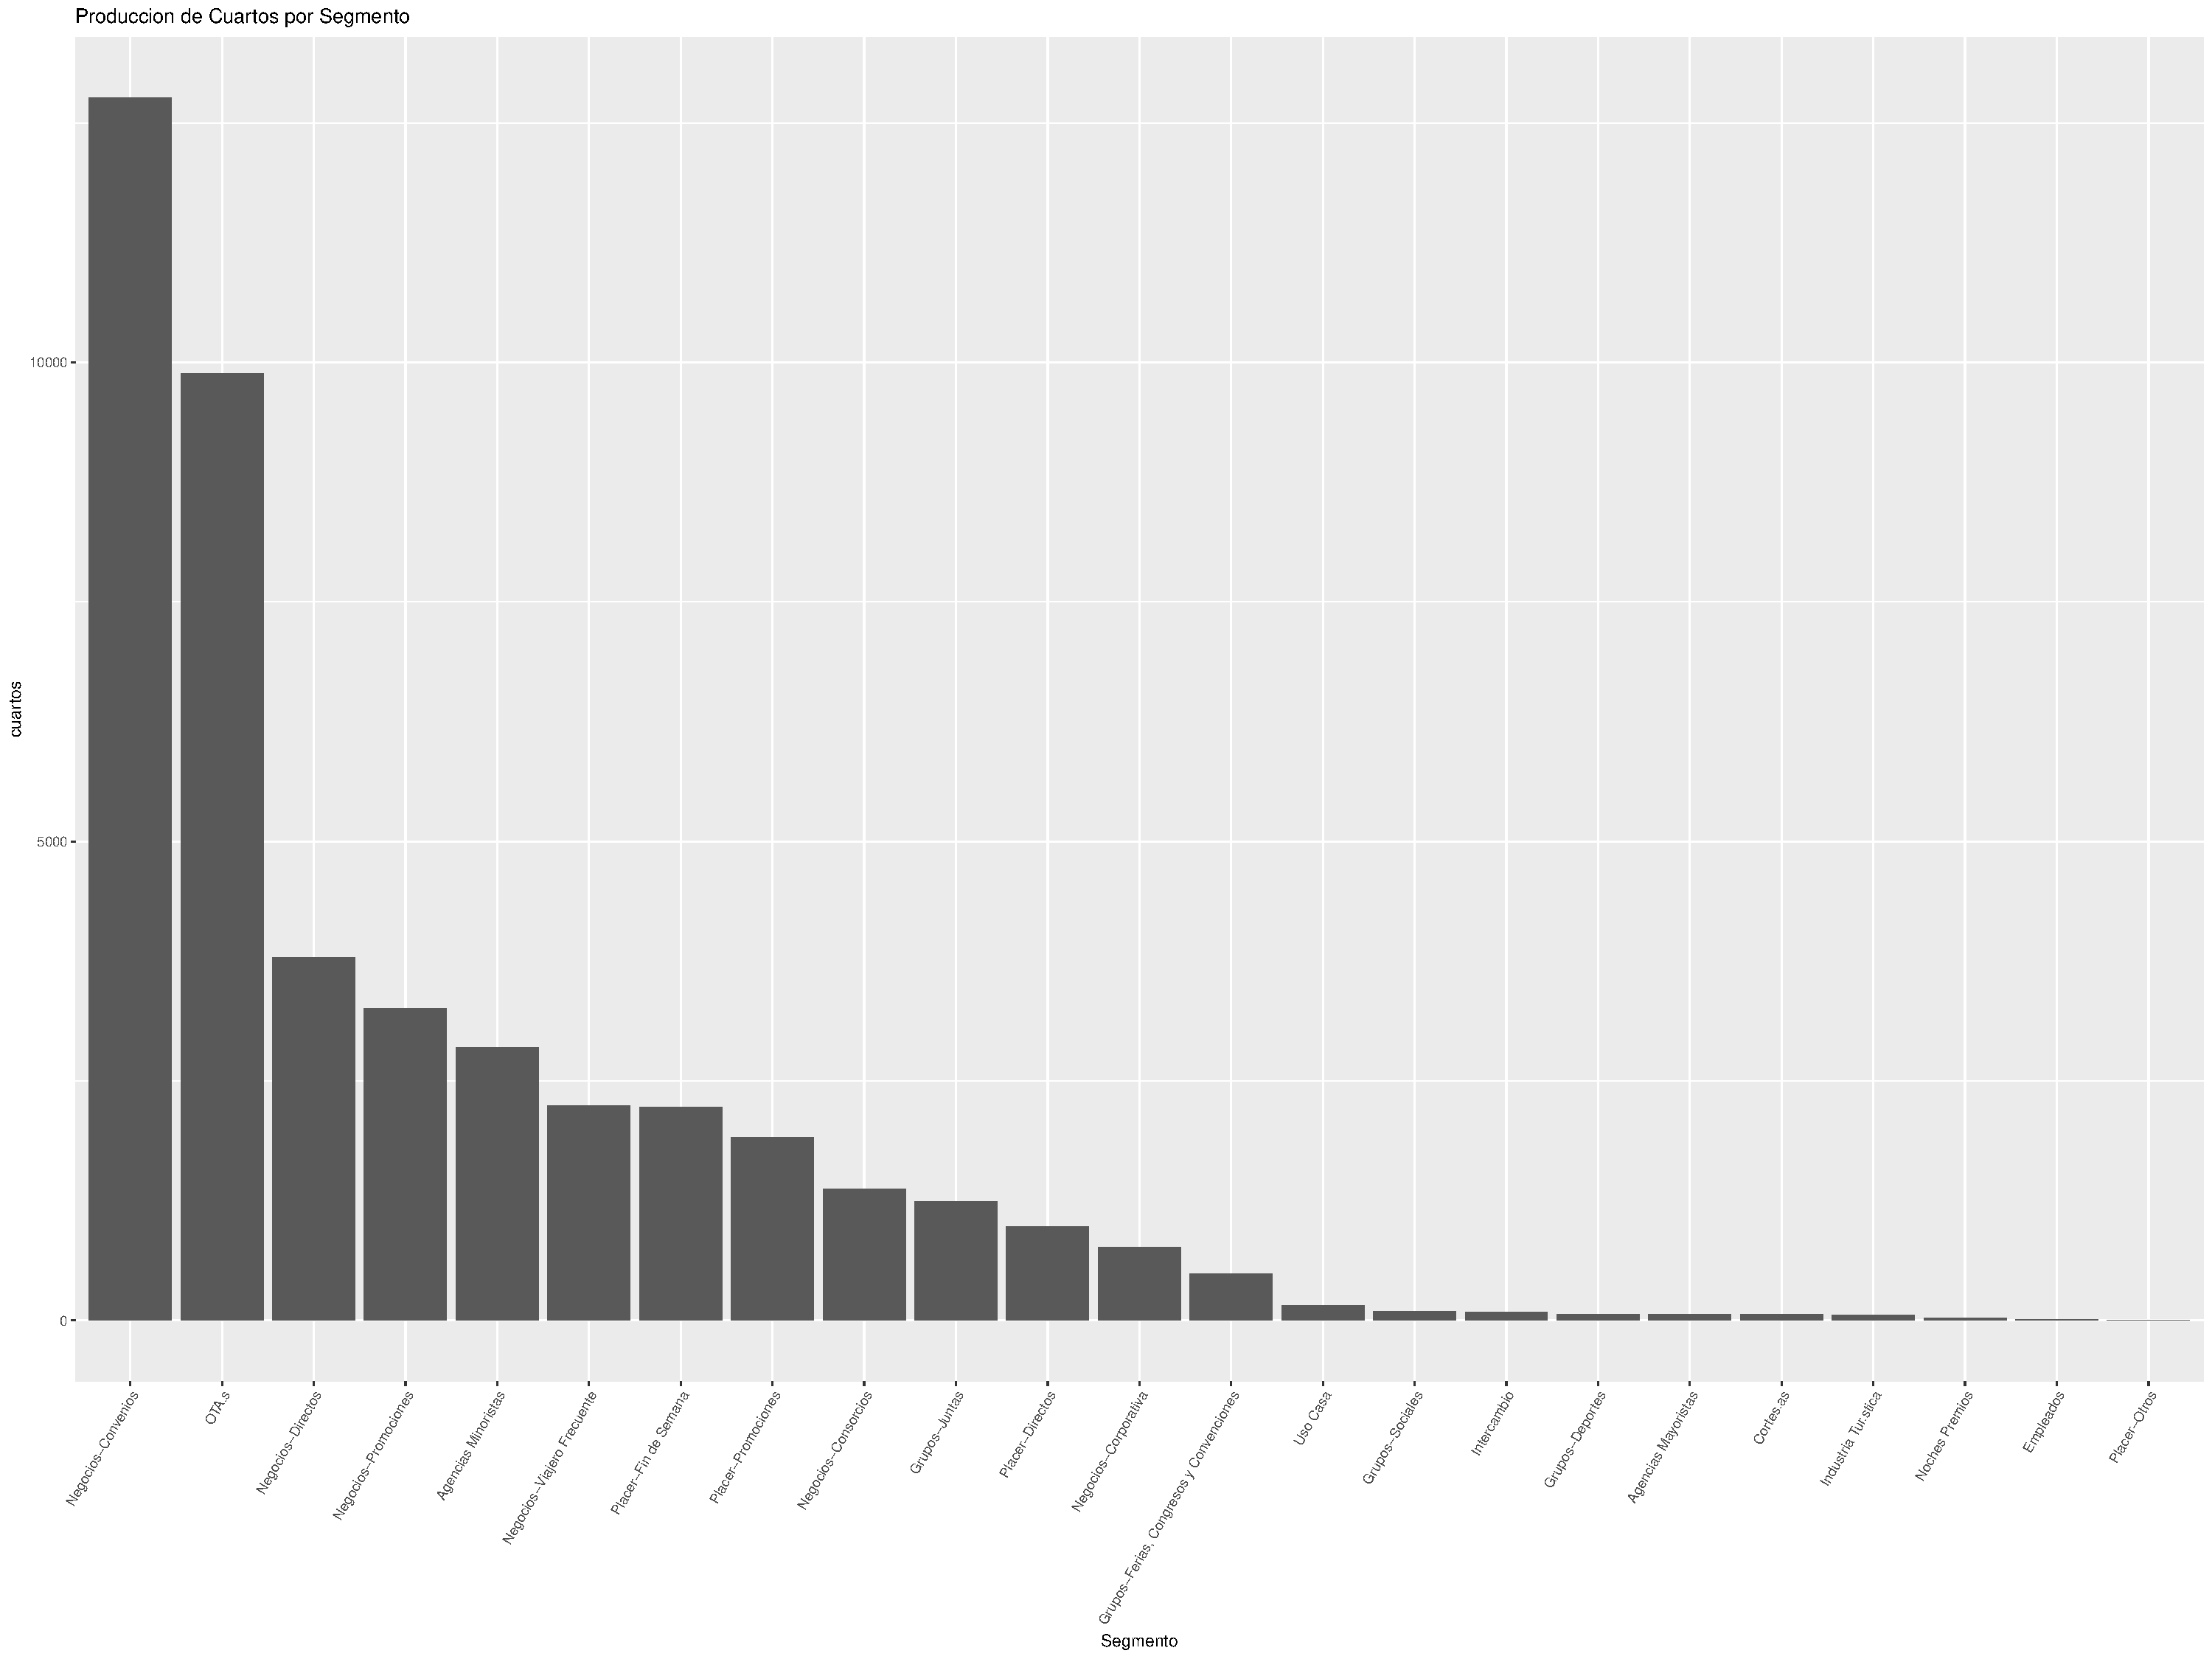
\includegraphics[width=\maxwidth]{figures/SegmentosMercadoCNO-1} 

\end{knitrout}
~\\
Podemos notar que el segmento de Negocios-Convenios produce más cuartos en un menor número de reservas, al contrario de las OTA's que producen mas reservaciones con menos venta de cuartos.
\paragraph{Estancia Promedio por Segmento} ~\\
A continuación graficaremos la estancia promedio de cada uno de los segmentos, esta medida nos deja ver cuantas noches pasa un huésped dentro de una propiedad. La fórmula para obtener esta variable es: $ Estancia\ Promedio=\frac{Cuartos Vendidos}{Reservas Generadas}$.
~\\
\begin{knitrout}
\definecolor{shadecolor}{rgb}{0.969, 0.969, 0.969}\color{fgcolor}
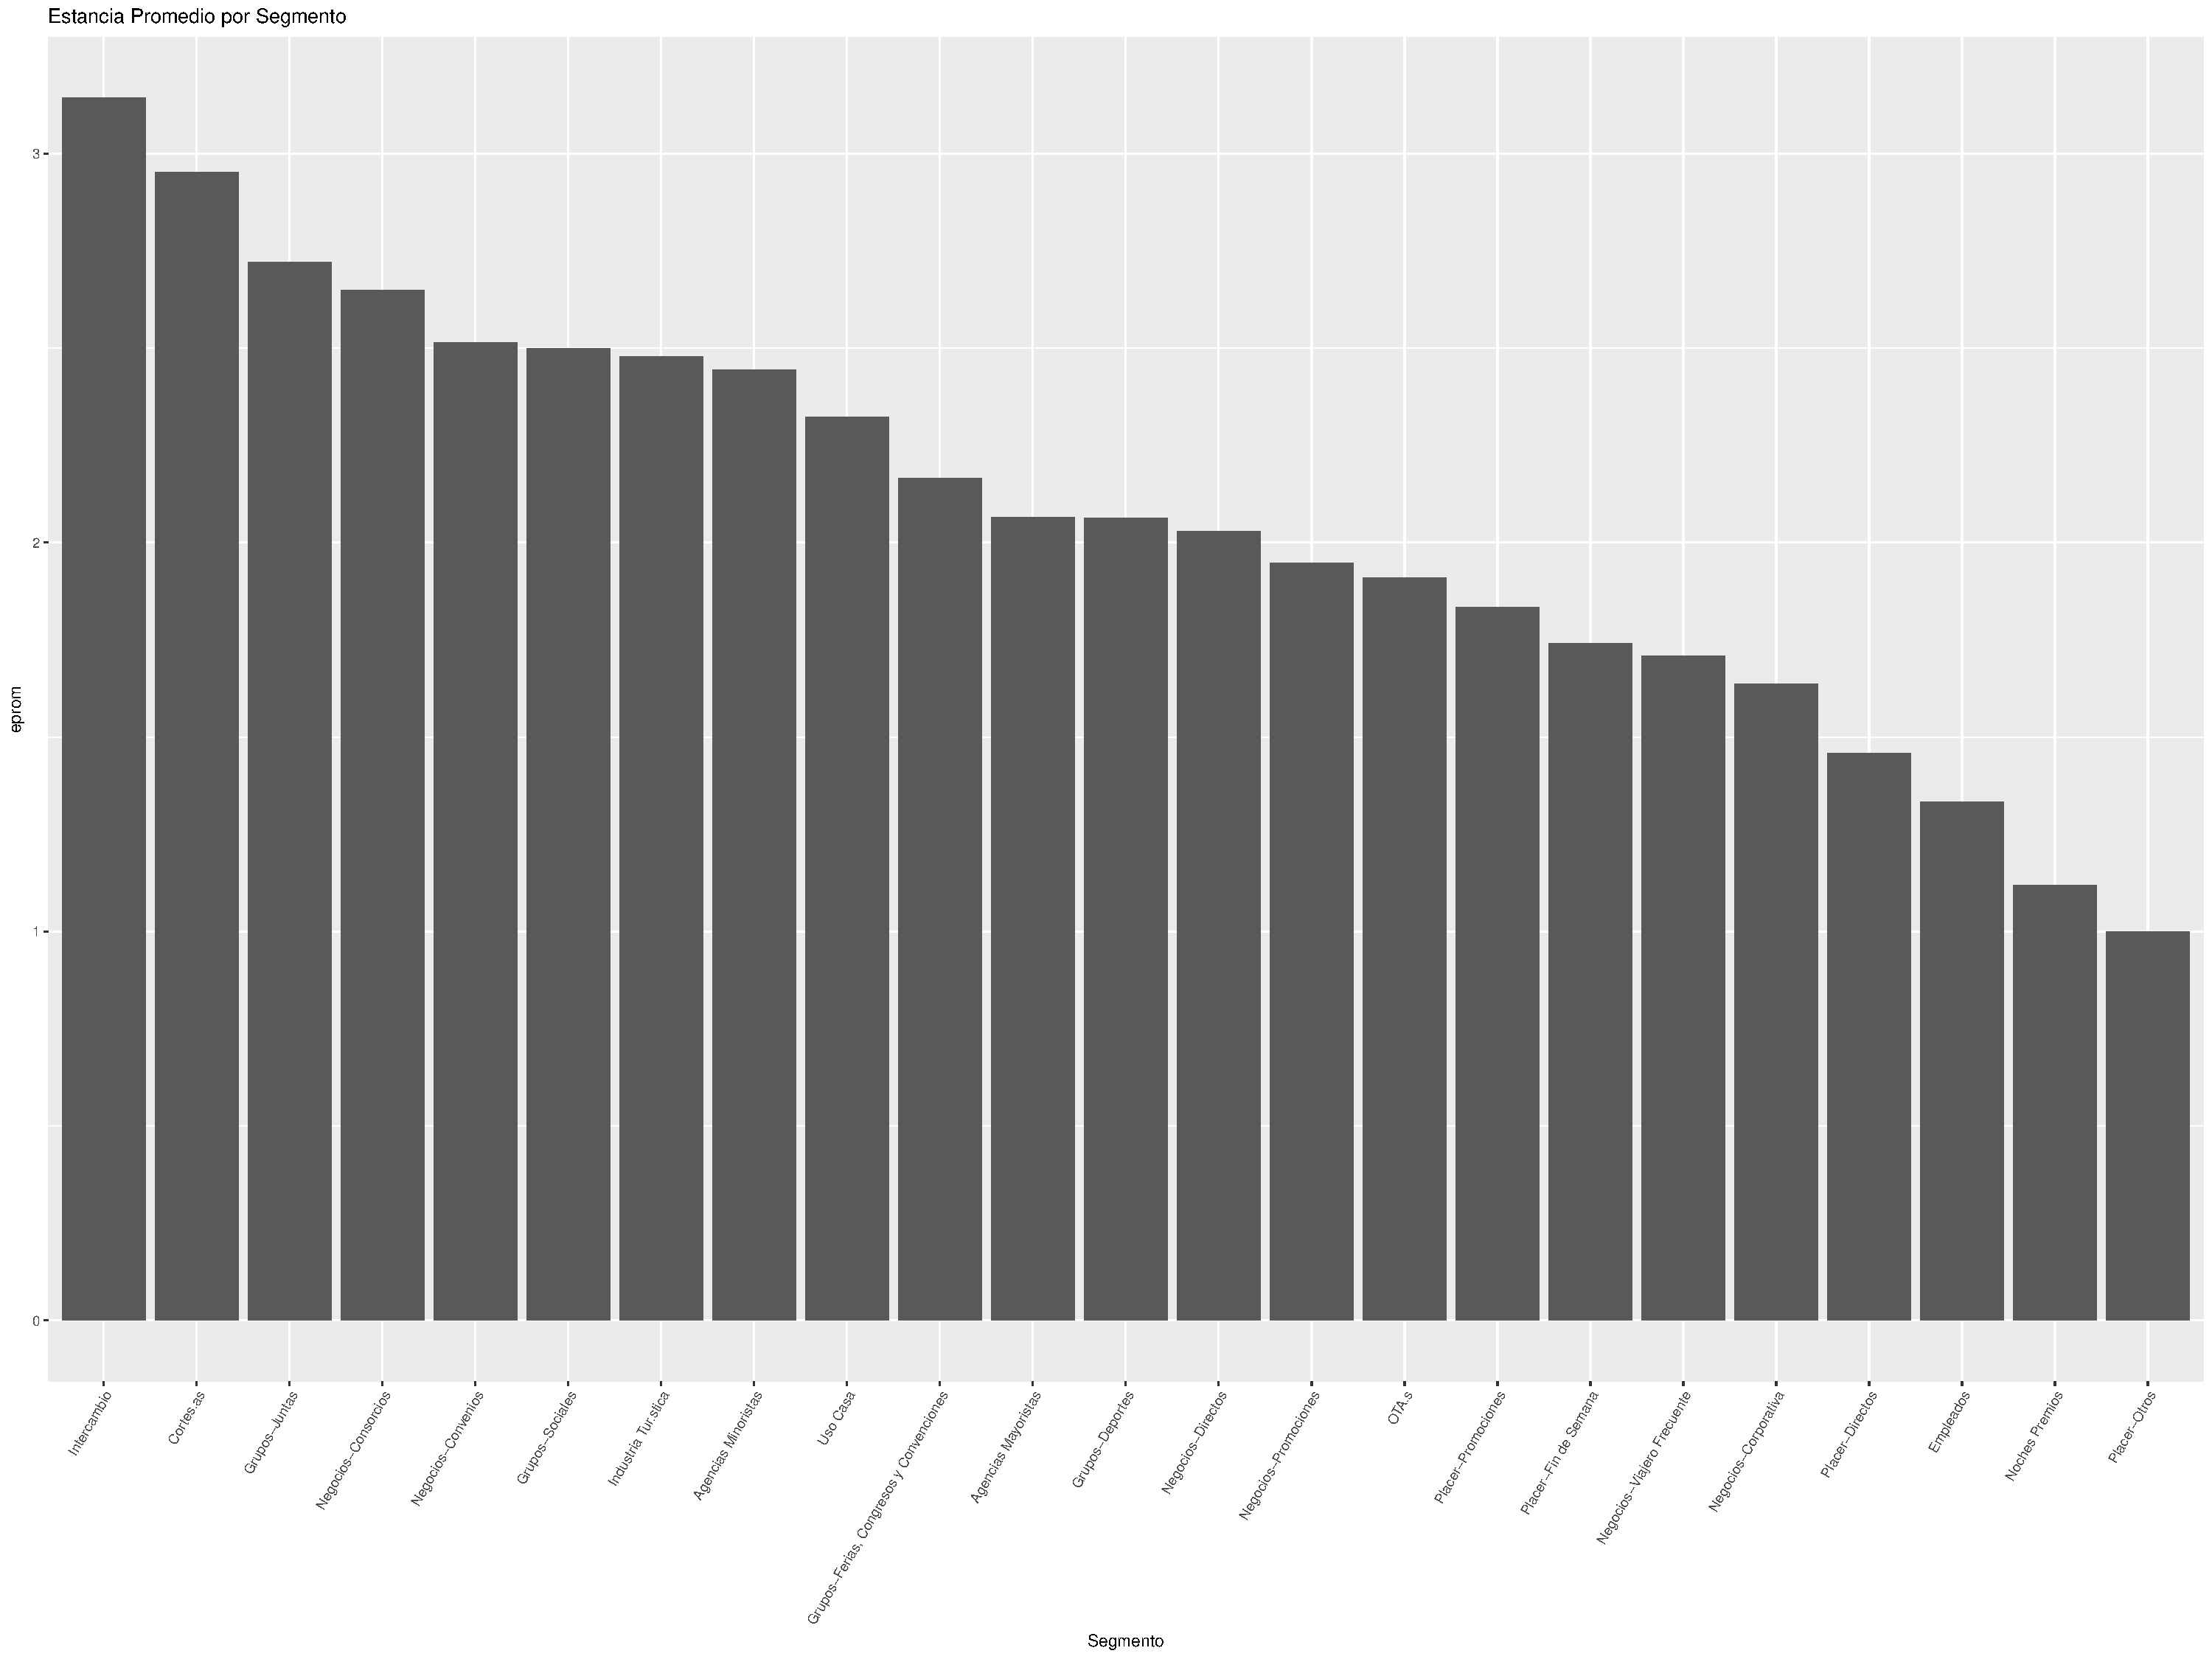
\includegraphics[width=\maxwidth]{figures/EstanciaPromedio-1} 

\end{knitrout}
~\\
Como podemos ver, la estancia promedio más alta la tiene el segmento de Negocios-Directos, con una estancia promedio de aproximadamente tres noches, contrastada con el segmento de Placer-Otros con una estancia promedio de aproximadamente noche. Esta información nos ayuda a complementar el perfil del huésped para esta propiedad ya que nos refuerza la idea de que el viajero de negocios utiliza las propiedades durante la semana laboral, y un viajero de placer puede que se hospede un día en fin de semana.
~\\
El segundo data set con el que contamos, trae información diaria sobre los níveles de ocupación, tarifa promedio, tarifa efectiva, habitaciones disponibles, penetración de ocupación y penetración de tarifa para los hoteles sujetos al estudio. Para efectos de este trabajo tomaremos información sobre el hotel con el que hemos venido trabajando.
\begin{knitrout}
\definecolor{shadecolor}{rgb}{0.969, 0.969, 0.969}\color{fgcolor}\begin{kframe}
\begin{verbatim}
##     Hotel               fecha                 occ        
##  Length:2049        Min.   :2013-01-01   Min.   :0.1447  
##  Class :character   1st Qu.:2014-05-28   1st Qu.:0.6478  
##  Mode  :character   Median :2015-10-22   Median :0.7987  
##                     Mean   :2015-10-22   Mean   :0.7786  
##                     3rd Qu.:2017-03-17   3rd Qu.:0.9811  
##                     Max.   :2018-08-11   Max.   :1.0063  
##    habs_disp         tp               po        
##  Min.   :159   Min.   :-267.6   Min.   :0.3158  
##  1st Qu.:159   1st Qu.:1046.1   1st Qu.:0.9592  
##  Median :159   Median :1154.8   Median :1.0583  
##  Mean   :159   Mean   :1227.6   Mean   :1.0709  
##  3rd Qu.:159   3rd Qu.:1344.8   3rd Qu.:1.1645  
##  Max.   :159   Max.   :2427.2   Max.   :2.3956  
##        pt               te        
##  Min.   :0.0000   Min.   :-228.9  
##  1st Qu.:0.9527   1st Qu.: 718.0  
##  Median :0.9941   Median : 979.4  
##  Mean   :1.0024   Mean   : 963.9  
##  3rd Qu.:1.0333   3rd Qu.:1159.7  
##  Max.   :8.0211   Max.   :2320.3
\end{verbatim}
\end{kframe}
\end{knitrout}
~\\
Lo primero que podemos observar es que contamos con datos para el hotel CEXXX a partir del "2013-01-01" y hasta el "2018-11-11". Esta propiedad tiene 159 habitaciones disponibles y maneja niveles de ocupación alrededor del 81.7\%; su tarifa promedio se encuentra alrededor de \$1486.60 y con PO y PT muy cercana a 1 indicando que es un hotel fuerte dentro del set competitivo de la plaza.
A continuación presentamos los datos de manera gráfica.
\paragraph{Ocupación en el tiempo} ~\\
\begin{knitrout}
\definecolor{shadecolor}{rgb}{0.969, 0.969, 0.969}\color{fgcolor}
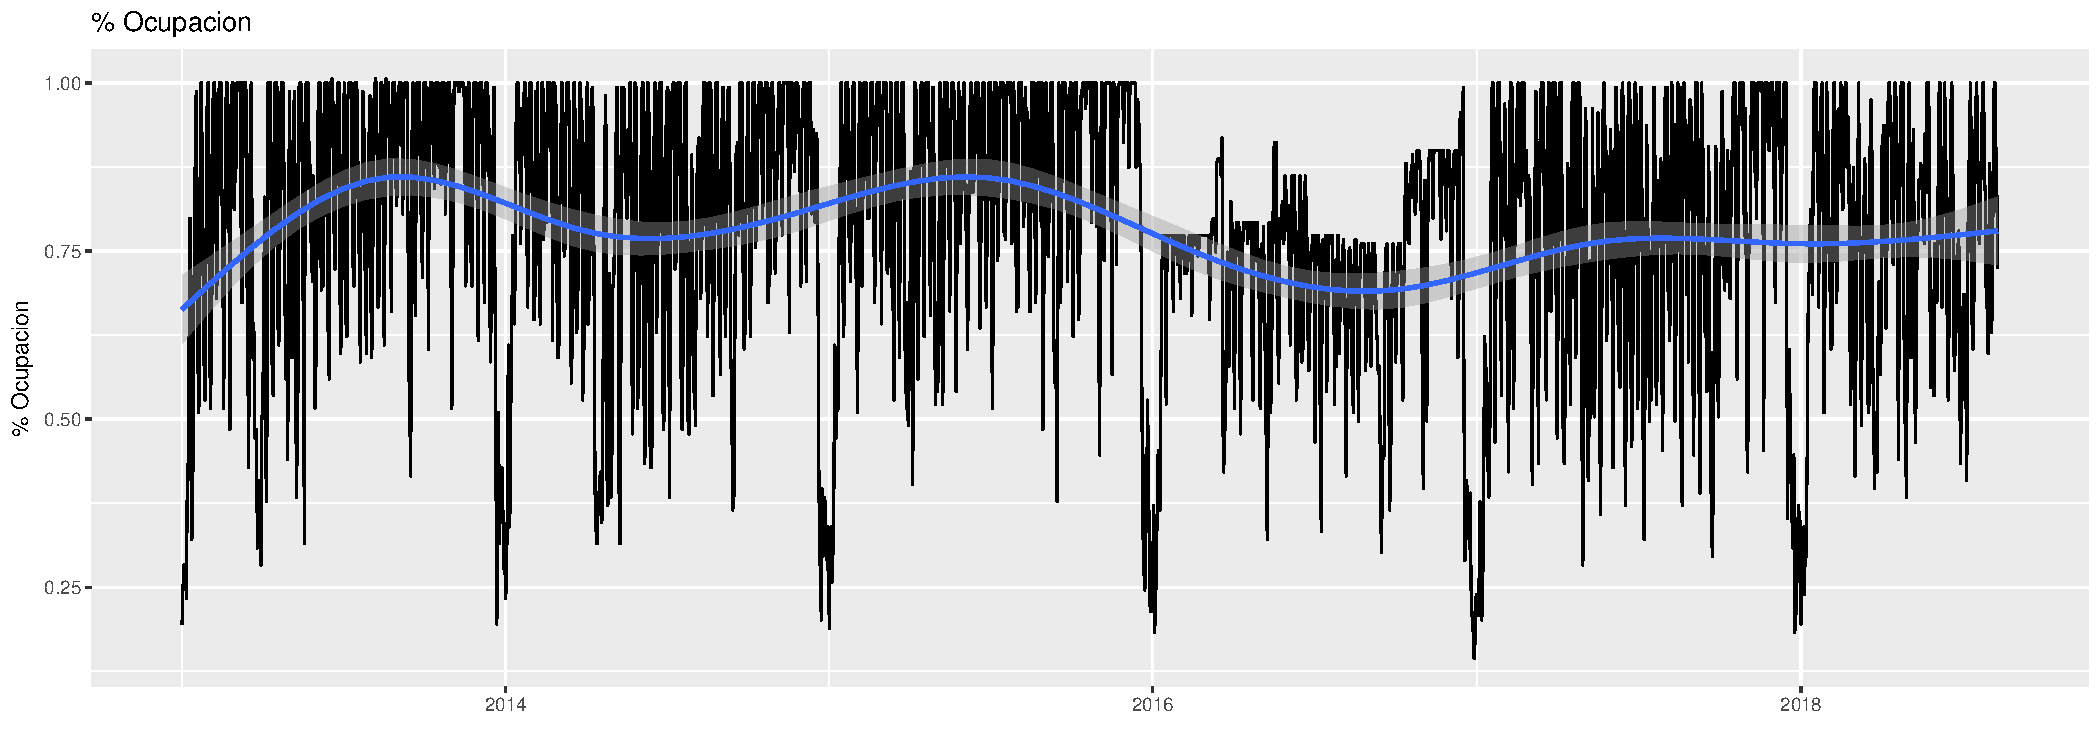
\includegraphics[width=\maxwidth]{figures/IndicadoresOcupacion-1} 

\end{knitrout}
\paragraph{Tarifa Promedio en el tiempo} ~\\
\begin{knitrout}
\definecolor{shadecolor}{rgb}{0.969, 0.969, 0.969}\color{fgcolor}
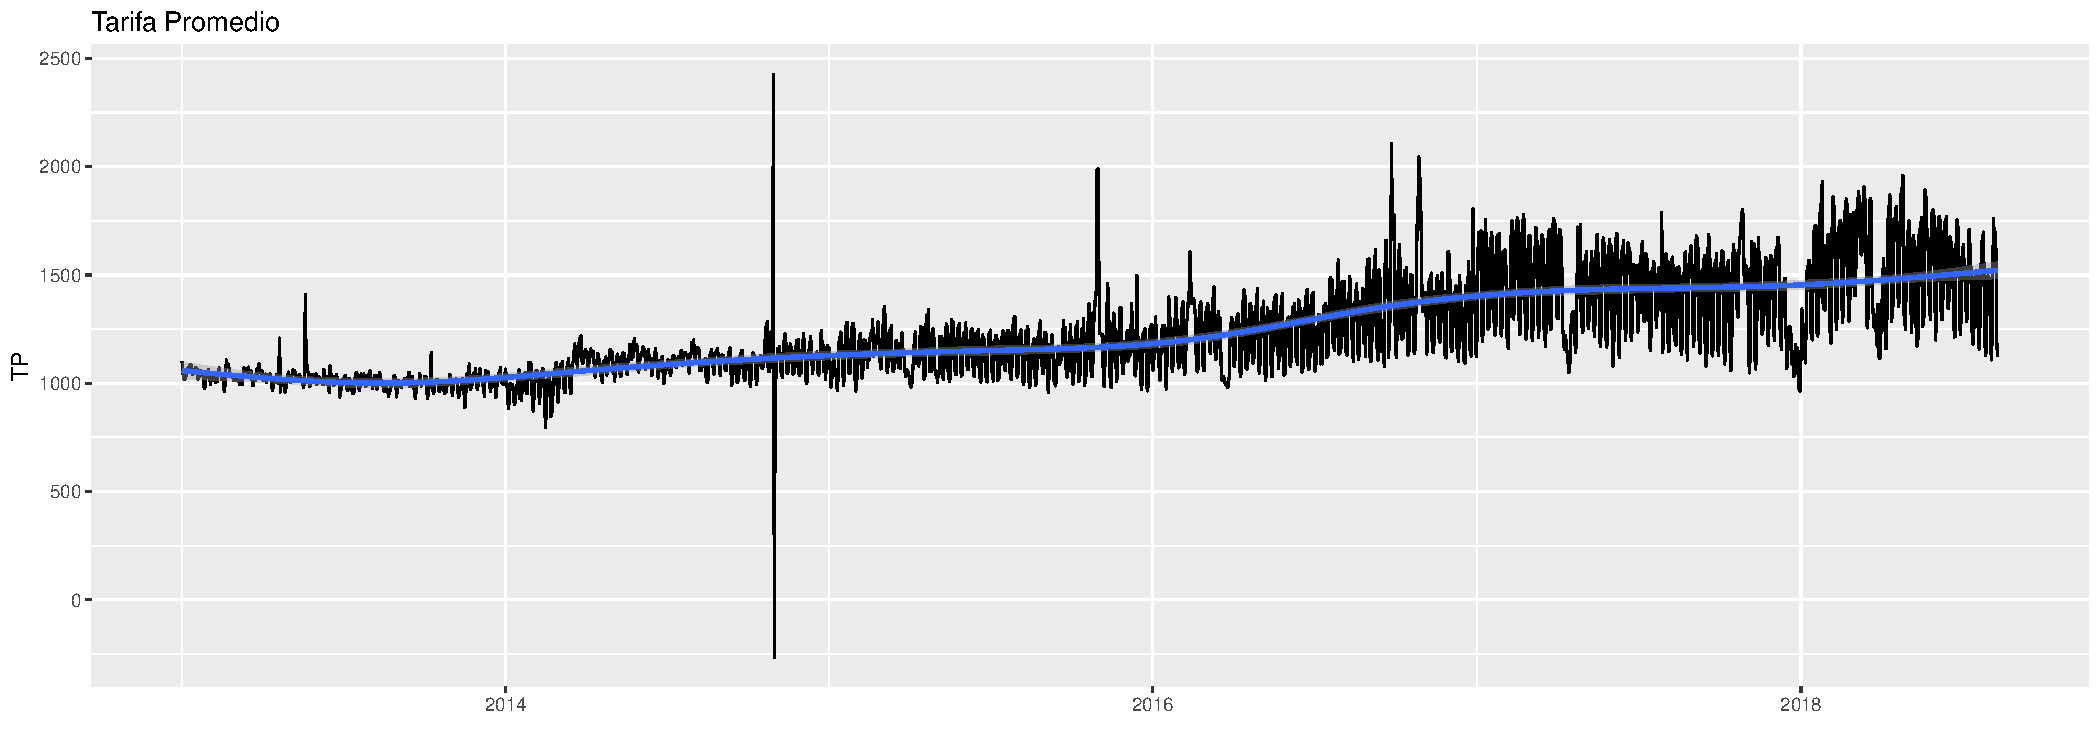
\includegraphics[width=\maxwidth]{figures/IndicadoresTarifaPromedio-1} 

\end{knitrout}
\paragraph{Penetración de Ocupación en el tiempo} ~\\
\begin{knitrout}
\definecolor{shadecolor}{rgb}{0.969, 0.969, 0.969}\color{fgcolor}
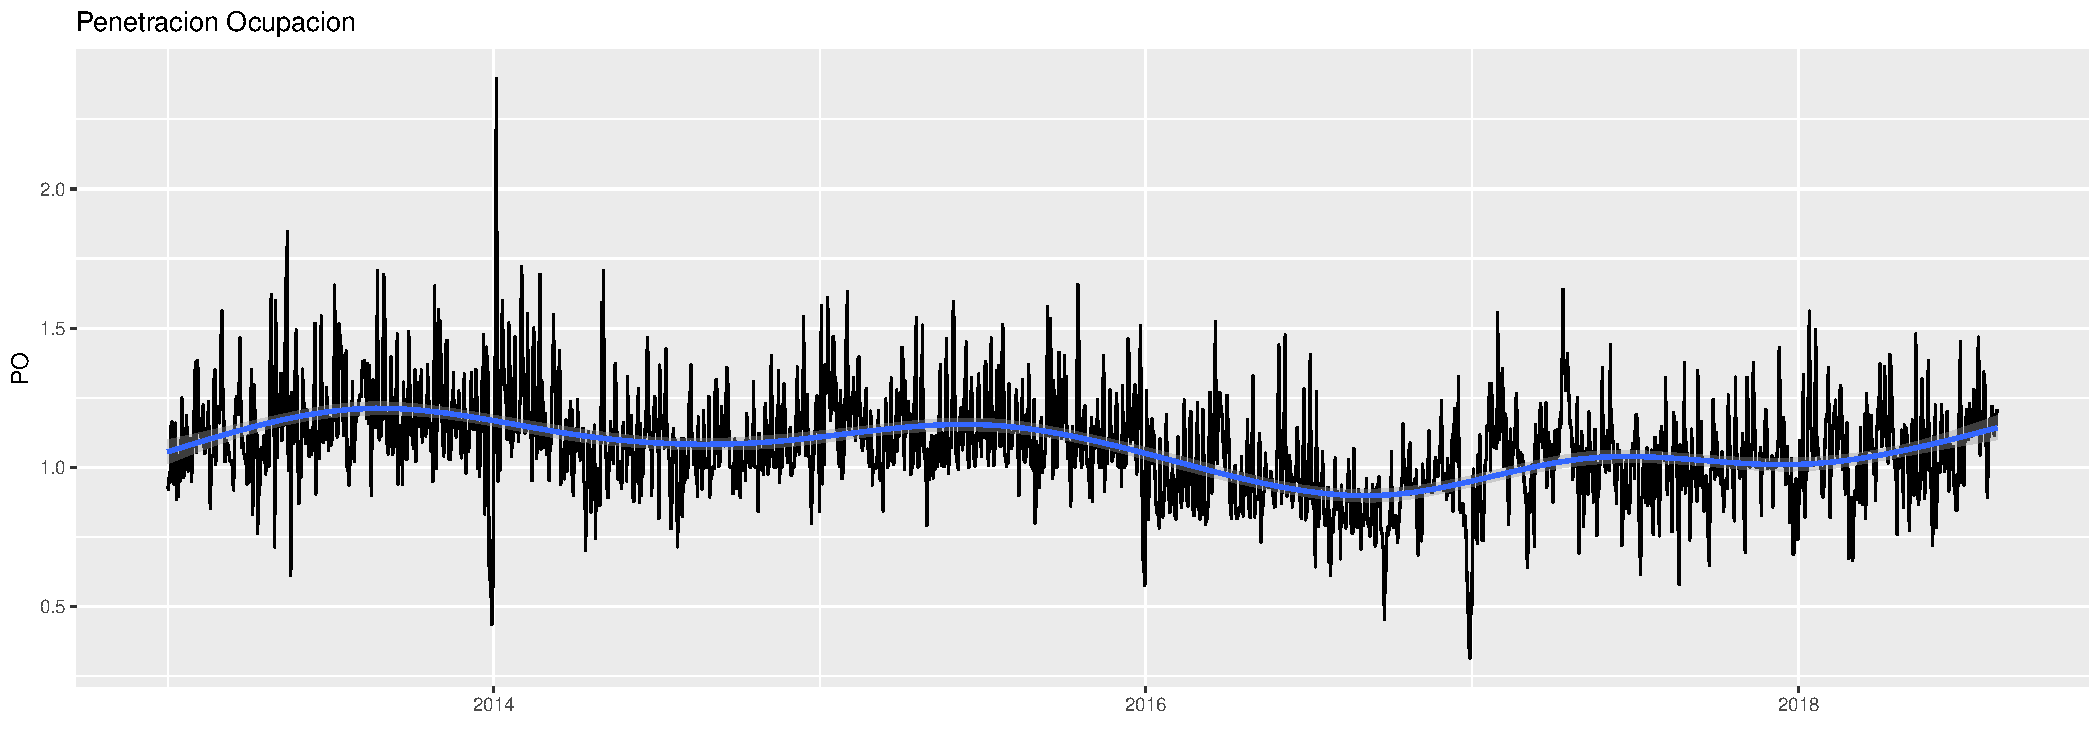
\includegraphics[width=\maxwidth]{figures/IndicadoresPO-1} 

\end{knitrout}
\paragraph{Penetración de Tarifa en el tiempo} ~\\
\begin{knitrout}
\definecolor{shadecolor}{rgb}{0.969, 0.969, 0.969}\color{fgcolor}
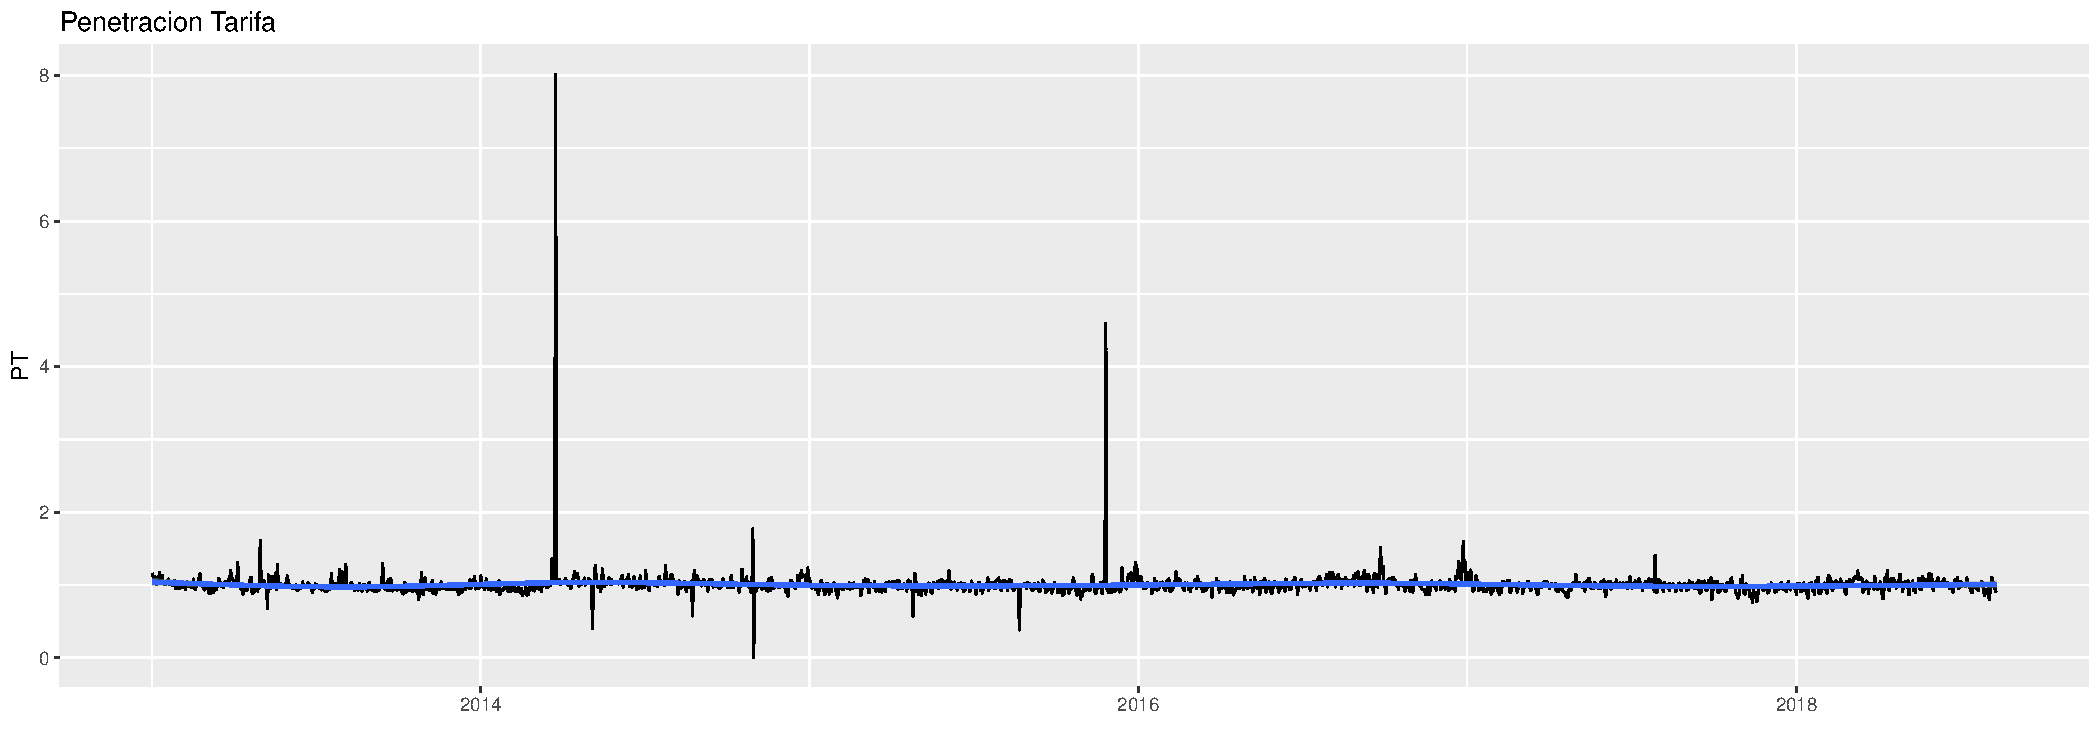
\includegraphics[width=\maxwidth]{figures/IndicadoresPT-1} 

\end{knitrout}
\paragraph{Penetración de Ocupación vs Penetración de Tarifa} ~\\
Al estudiar los datos notamos que hay una correlación negativa entre la penetración de ocupación y la penetración de la tarifa, recordemos que la primera indica cuanta ocupación tiene una de las propiedades de CityExpress con respecto a la ocupación de su plaza, y la segunda indica cuánto del ingreso disponible se está quedando dentro de la propiedad de interés. En otras palabras podemos pensar en una relación similar a la del precio de un bien vs la demanda de un bien. A mayor precio menor demanda y a menor precio mayor demanda, lo cual indica que la relación entre ambas variables debe ser negativa.
~\\
\begin{knitrout}
\definecolor{shadecolor}{rgb}{0.969, 0.969, 0.969}\color{fgcolor}
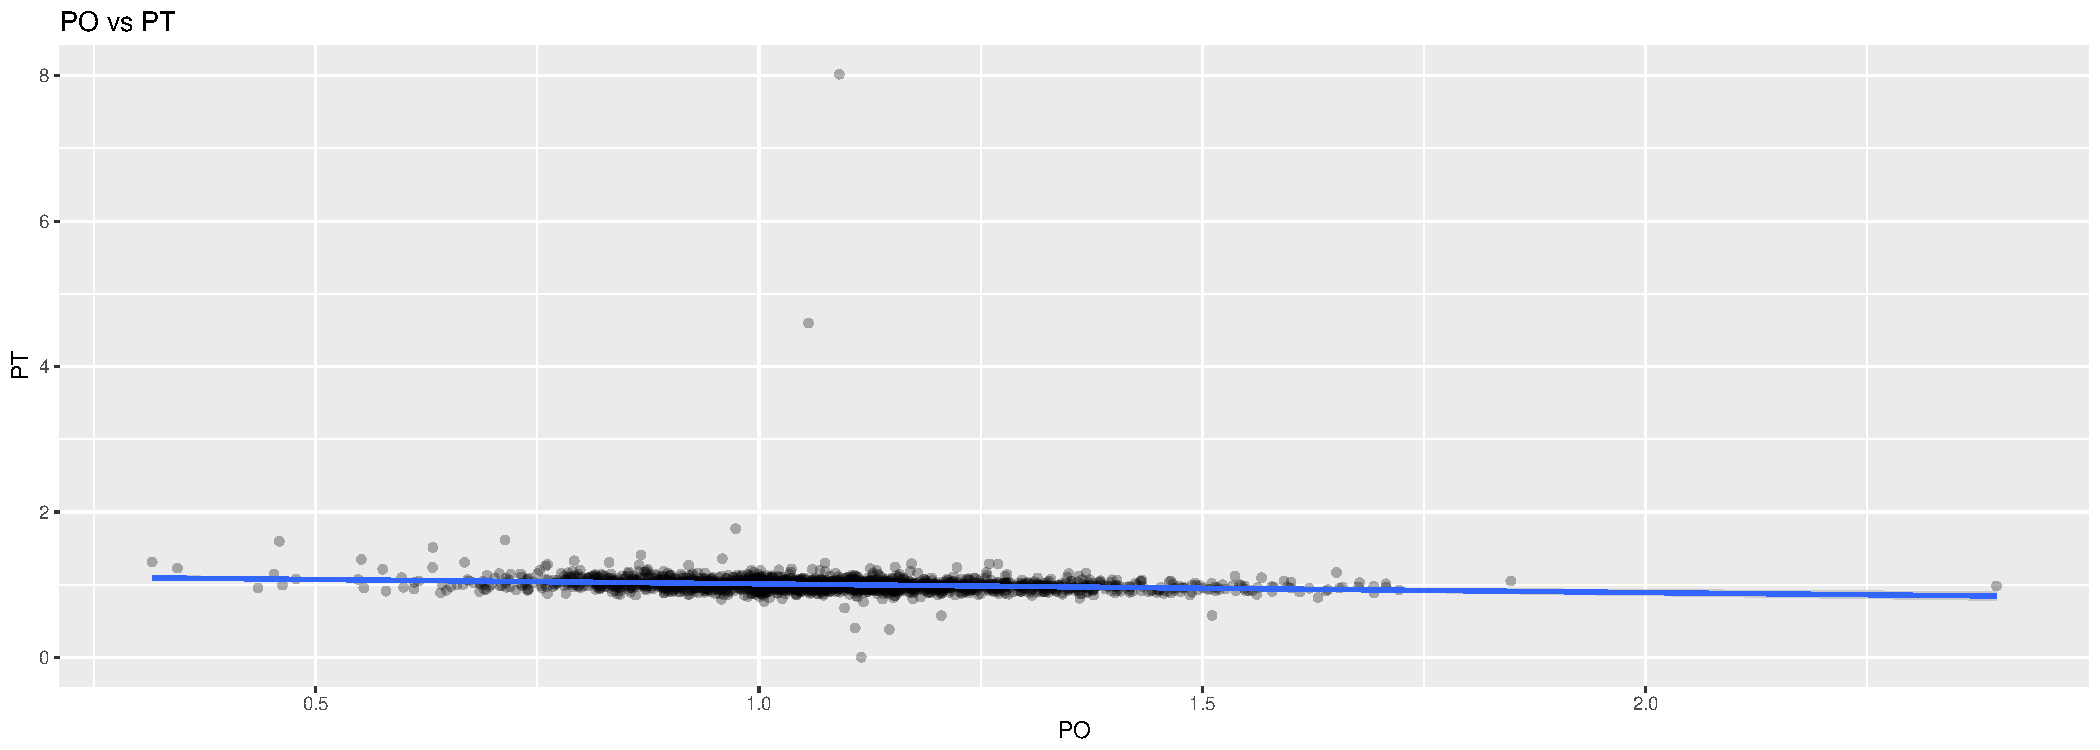
\includegraphics[width=\maxwidth]{figures/POvsPT-1} 

\end{knitrout}
\paragraph{Precio de la competencia} ~\\
Para este proyecto contamos con un dataset que contiene información sobre los precios de la competencia definida para CEXXX publicados en las agencias de viajes en línea.
~\\
\begin{knitrout}
\definecolor{shadecolor}{rgb}{0.969, 0.969, 0.969}\color{fgcolor}\begin{kframe}
\begin{verbatim}
##     nombre              fecha                precio     
##  Length:5109        Min.   :2017-10-13   Min.   :  794  
##  Class :character   1st Qu.:2018-03-22   1st Qu.: 1399  
##  Mode  :character   Median :2018-08-29   Median : 1650  
##                     Mean   :2018-08-29   Mean   : 2244  
##                     3rd Qu.:2019-02-05   3rd Qu.: 2122  
##                     Max.   :2019-08-10   Max.   :85572
\end{verbatim}
\end{kframe}
\end{knitrout}
\paragraph{Precios en el tiempo} ~\\
\begin{knitrout}
\definecolor{shadecolor}{rgb}{0.969, 0.969, 0.969}\color{fgcolor}
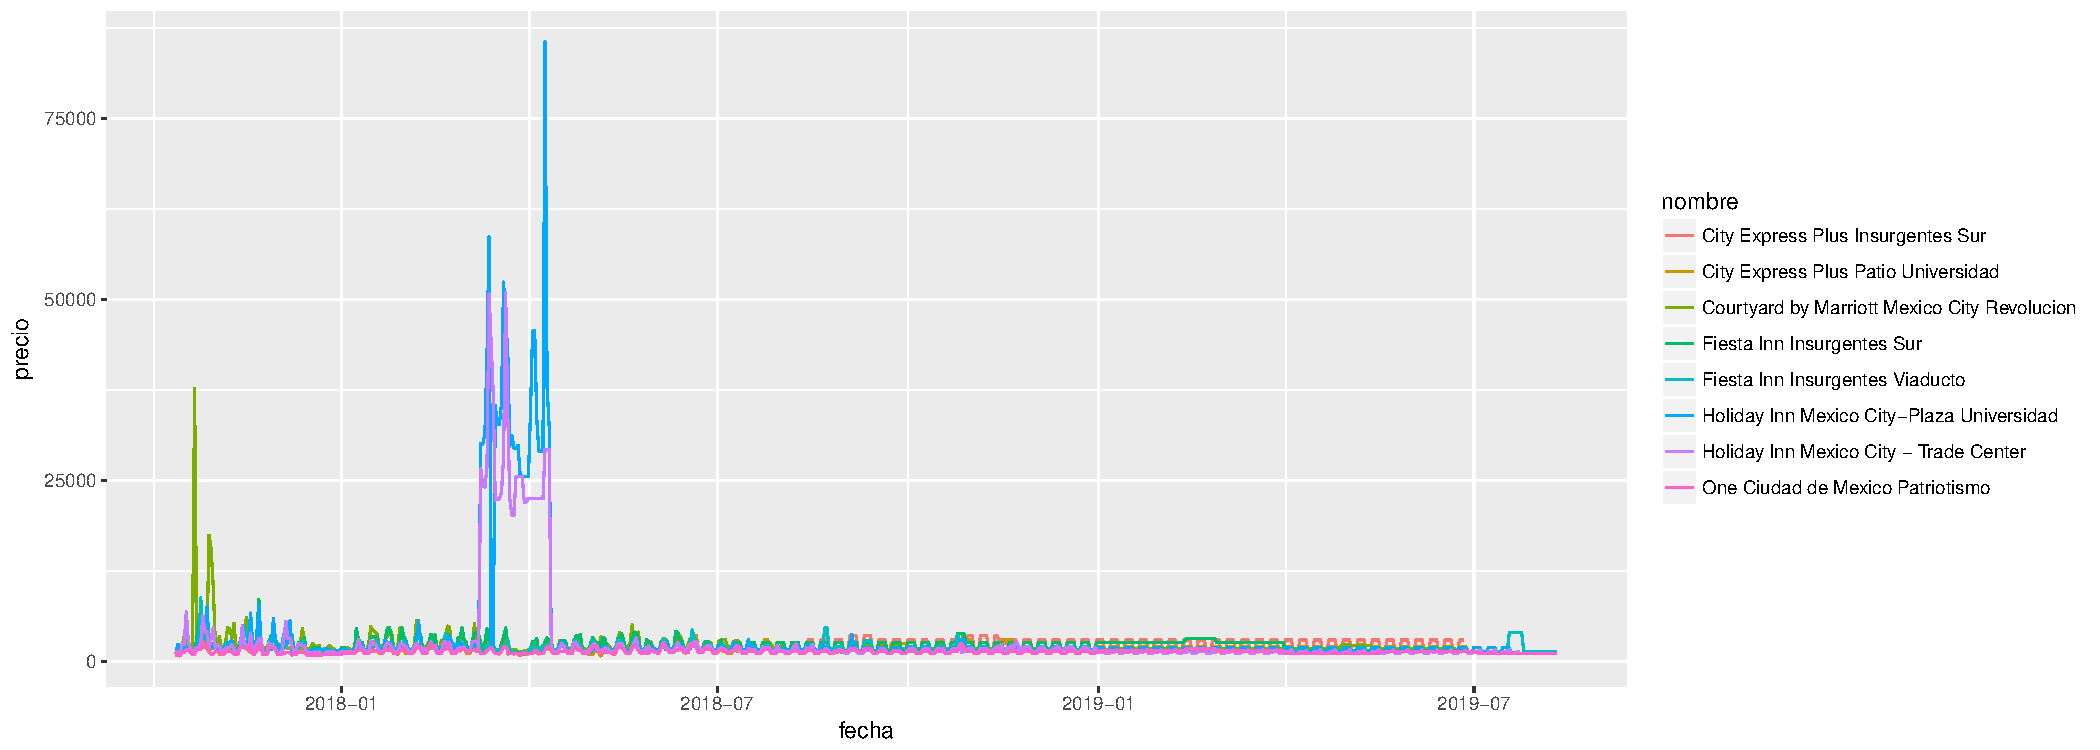
\includegraphics[width=\maxwidth]{figures/PreciosGraf-1} 

\end{knitrout}
~\\
Nos llaman la atención algunos datos que salen del patrón del comportamiento, para estudiarlos con mas detalle veamos la siguiente gráfica:
~\\
\begin{knitrout}
\definecolor{shadecolor}{rgb}{0.969, 0.969, 0.969}\color{fgcolor}
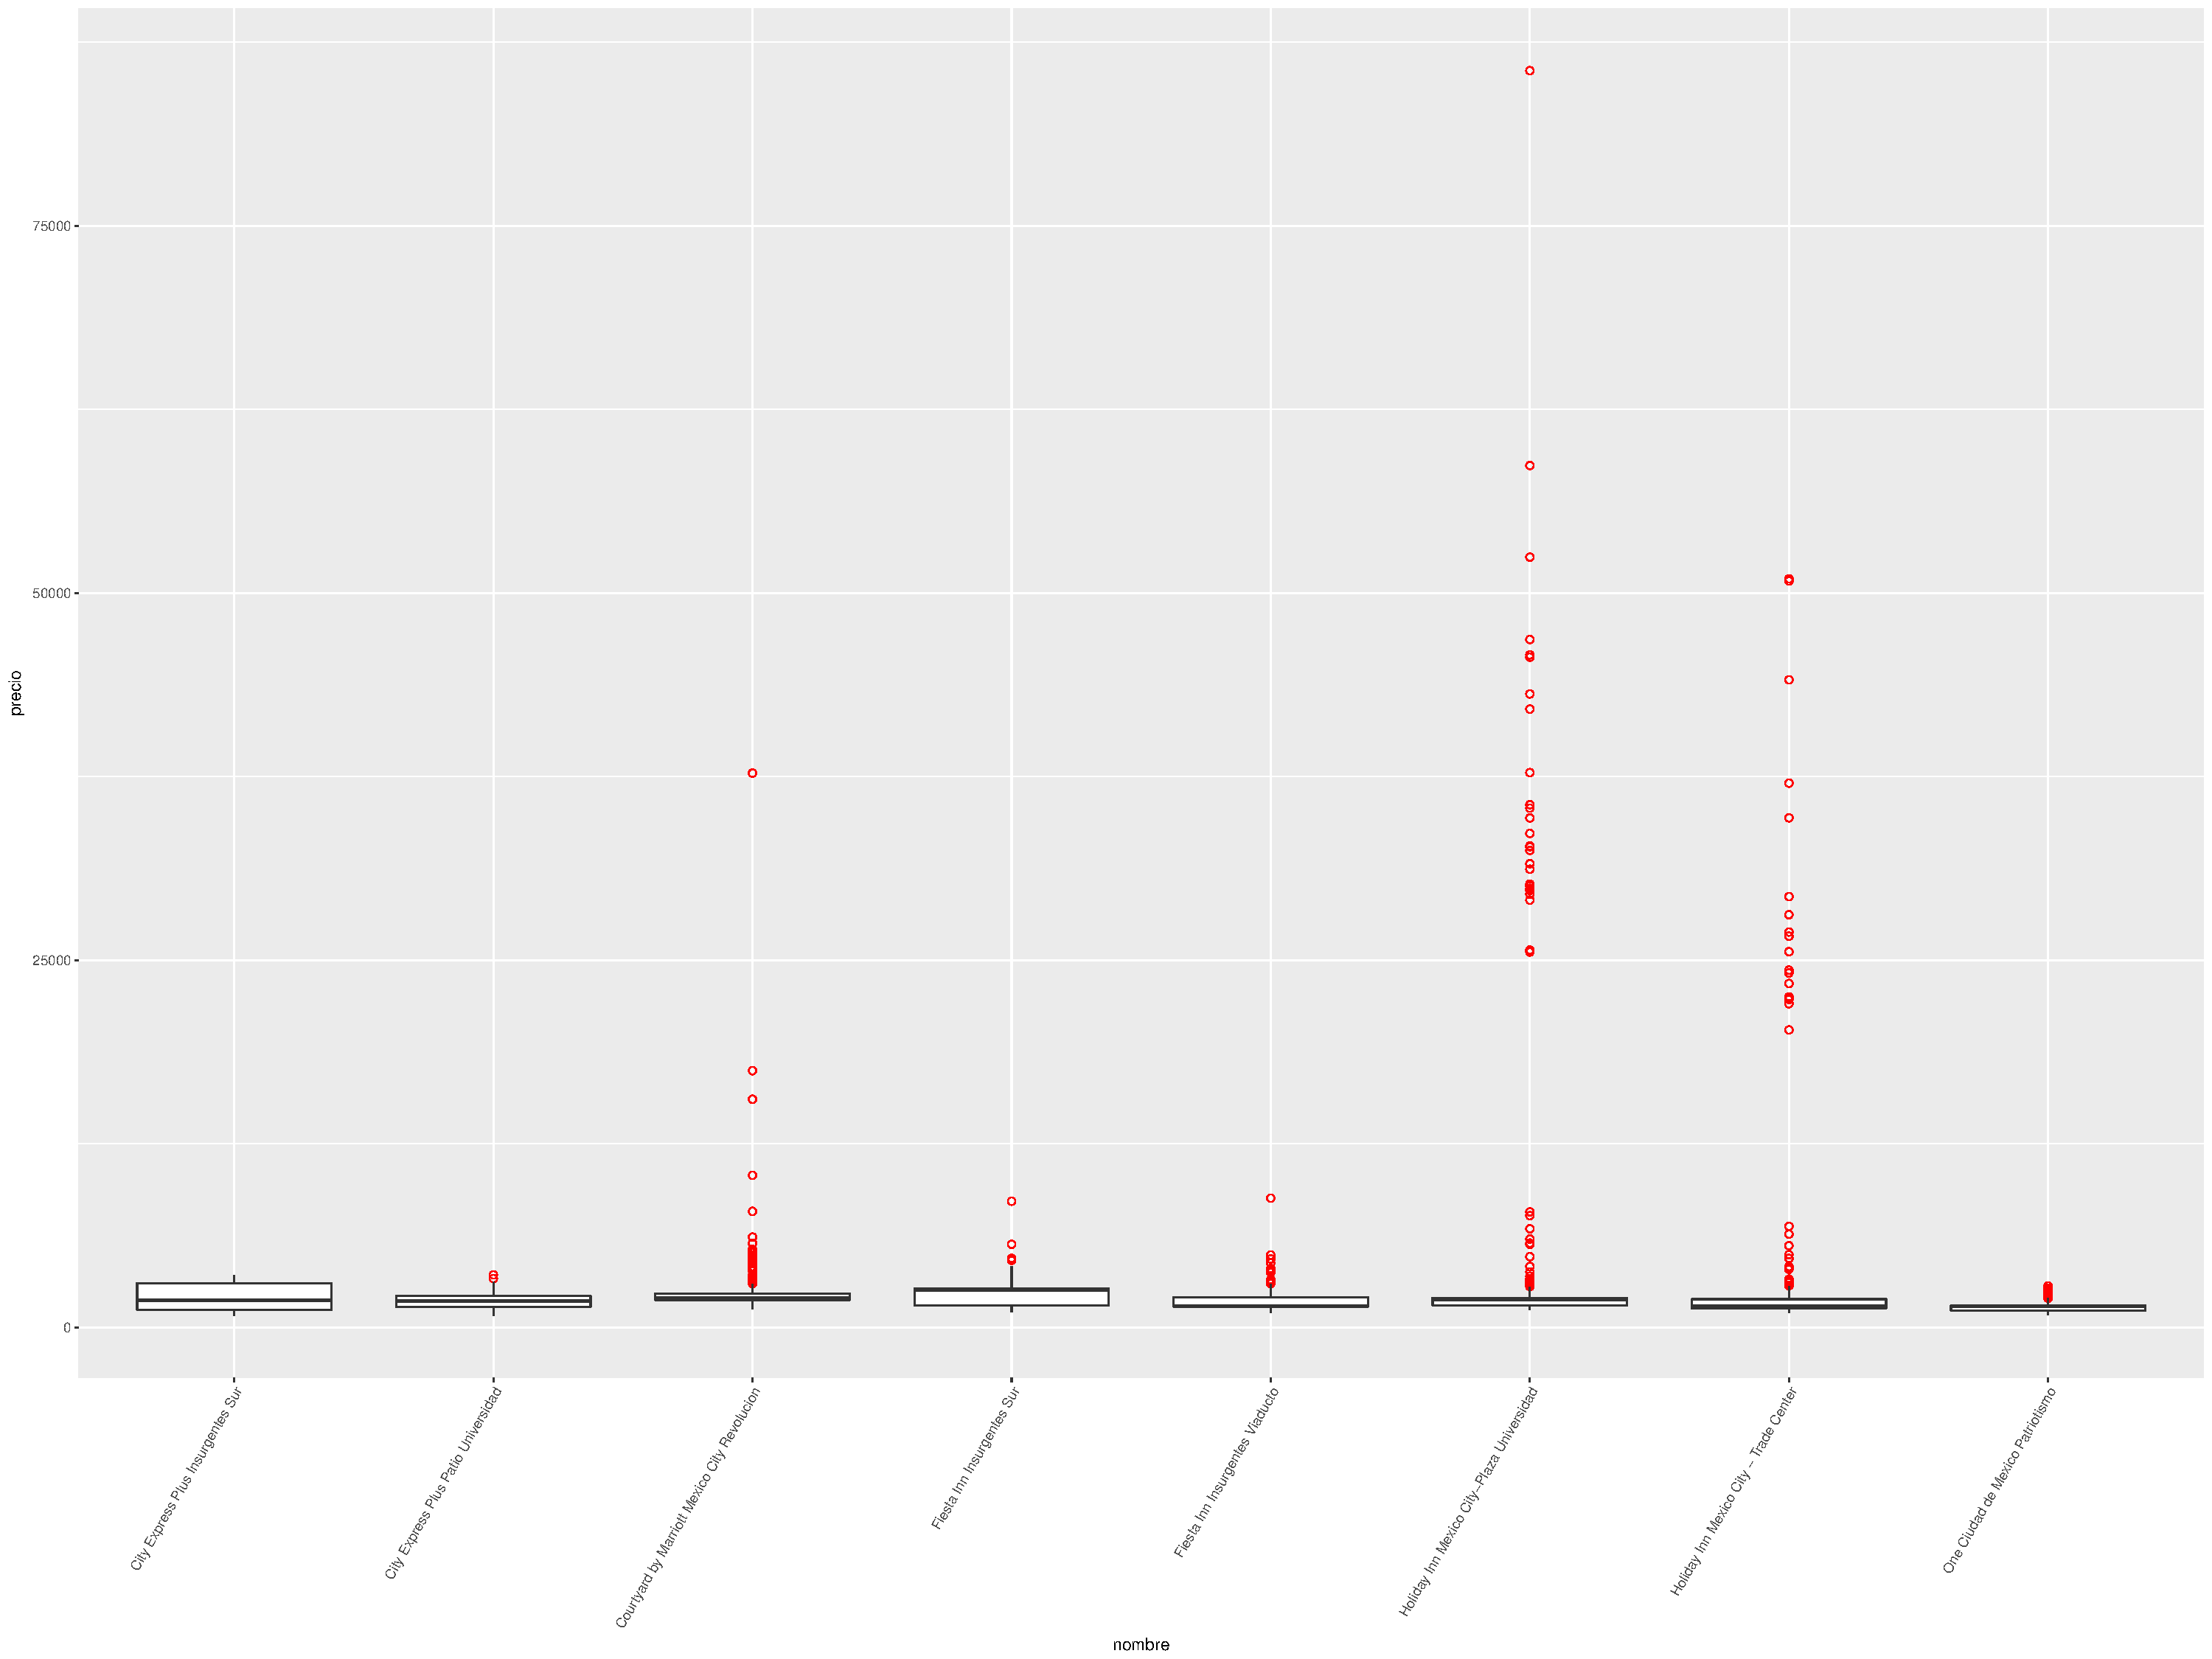
\includegraphics[width=\maxwidth]{figures/PreciosBoxPlot-1} 

\end{knitrout}
~\\
Podemos observar que este data set contiene datos atípicos, por ejemplo los hoteles "Courtyard by Marriot Mexico City Revolución", "Holiday Inn Mexico City-Plaza Universidad" y "Holiday Inn Mexico City - Trade Center" tienen tarifas arriba de los \$10,000 MXN, lo cual es poco probable ya que son hoteles que compiten directamente con CityExpress y su mercado es el mismo (Viajero de Negocios). Estos casos se deberán tomarse en cuenta al momento de construír el modelo de pronóstico y pricing dinámico para evitar resultados erróneos. 
\paragraph{Precios publicos}
Estudiaremos también los precios públicos para la propiedad que esta siendo sujeta al análisis
\begin{knitrout}
\definecolor{shadecolor}{rgb}{0.969, 0.969, 0.969}\color{fgcolor}\begin{kframe}
\begin{verbatim}
##   prop_code           rate_start           rate_key        
##  Length:575         Min.   :2017-01-01   Length:575        
##  Class :character   1st Qu.:2017-05-24   Class :character  
##  Mode  :character   Median :2017-10-15   Mode  :character  
##                     Mean   :2017-10-20                     
##                     3rd Qu.:2018-03-20                     
##                     Max.   :2018-08-11                     
##   curr_code           price_1pax  
##  Length:575         Min.   :1050  
##  Class :character   1st Qu.:1200  
##  Mode  :character   Median :1500  
##                     Mean   :1641  
##                     3rd Qu.:1950  
##                     Max.   :3200
\end{verbatim}
\end{kframe}
\end{knitrout}
\paragraph{Precios publicos en el tiempo} ~\\
\begin{knitrout}
\definecolor{shadecolor}{rgb}{0.969, 0.969, 0.969}\color{fgcolor}
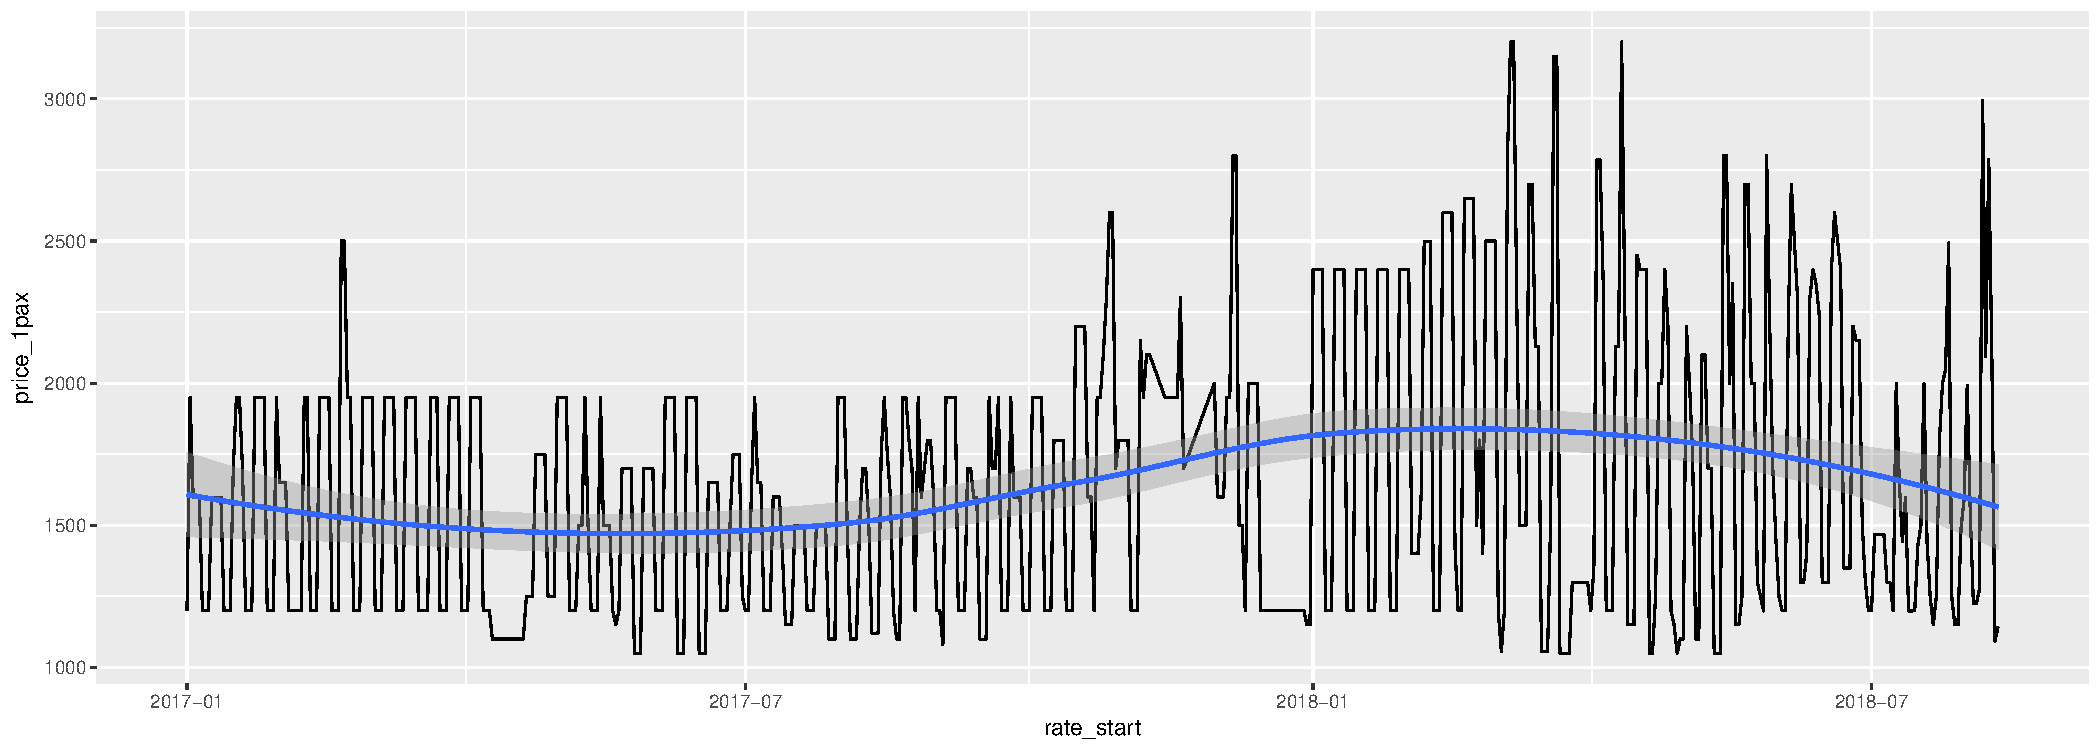
\includegraphics[width=\maxwidth]{figures/PreciospubGraf-1} 

\end{knitrout}
~\\
\begin{knitrout}
\definecolor{shadecolor}{rgb}{0.969, 0.969, 0.969}\color{fgcolor}
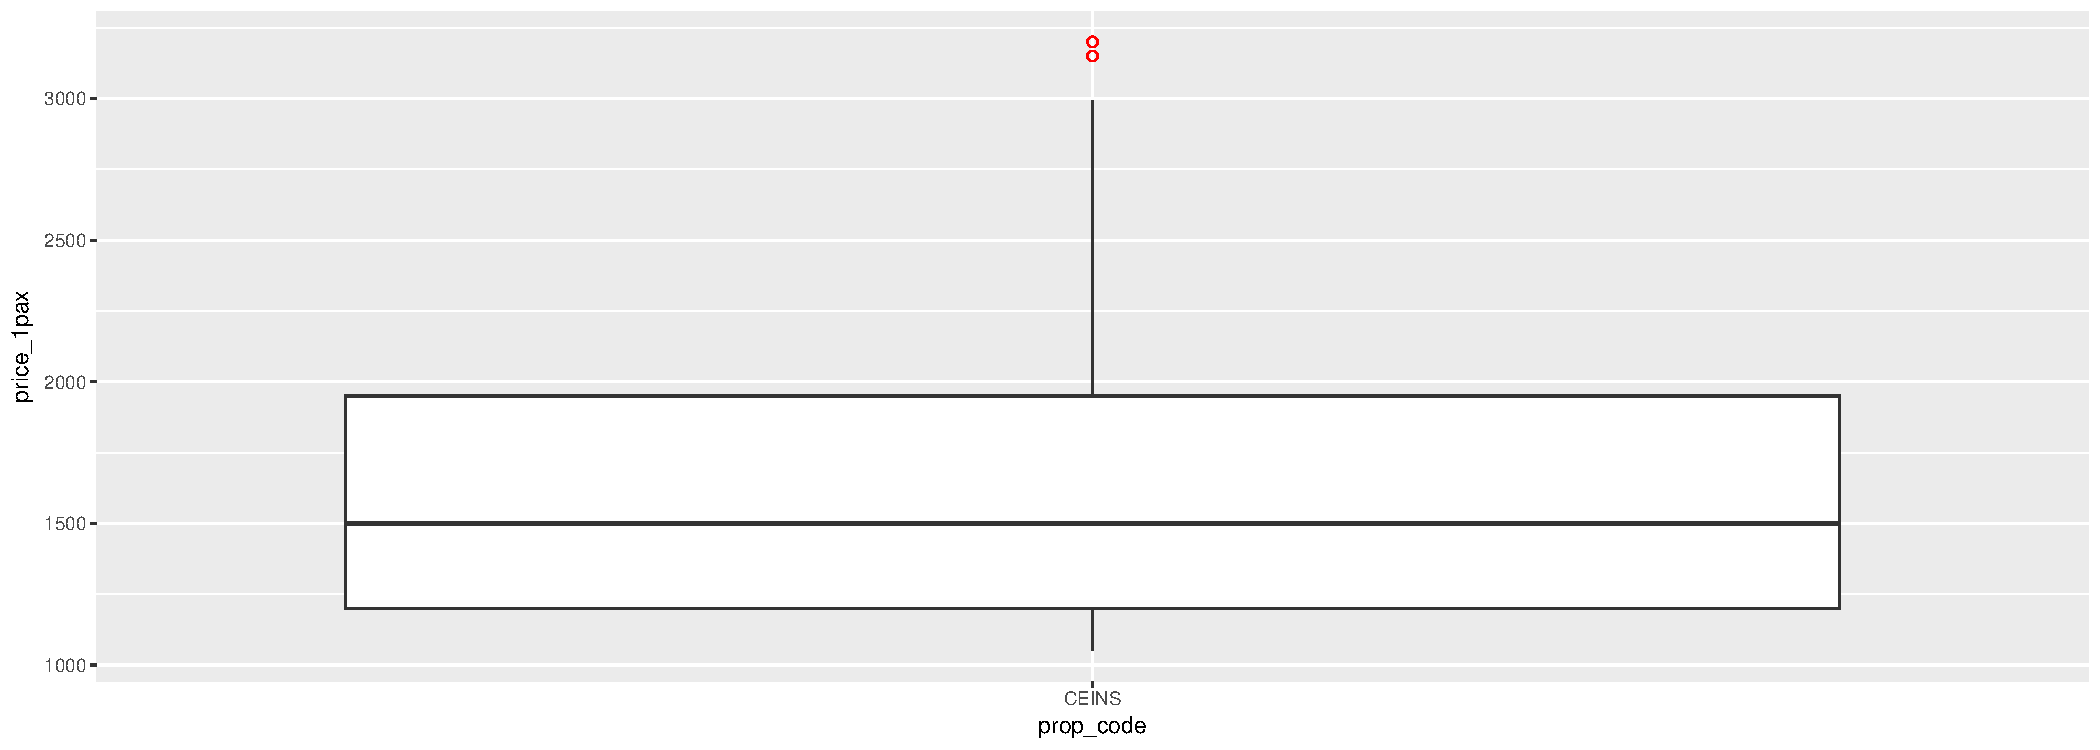
\includegraphics[width=\maxwidth]{figures/Boxplotpubprice-1} 

\end{knitrout}
~\\
\paragraph{Calidad}
~\\
\begin{knitrout}
\definecolor{shadecolor}{rgb}{0.969, 0.969, 0.969}\color{fgcolor}\begin{kframe}
\begin{verbatim}
##     plaza              hotel              calidad     
##  Length:779         Length:779         Min.   :0.000  
##  Class :character   Class :character   1st Qu.:3.400  
##  Mode  :character   Mode  :character   Median :4.000  
##                                        Mean   :3.596  
##                                        3rd Qu.:4.400  
##                                        Max.   :5.000
\end{verbatim}
\end{kframe}
\end{knitrout}
~\\
\paragraph{Calidad vs Precio}
~\\
\begin{knitrout}
\definecolor{shadecolor}{rgb}{0.969, 0.969, 0.969}\color{fgcolor}\begin{kframe}


{\ttfamily\noindent\bfseries\color{errorcolor}{\#\# Error in convertUnit(x, unitTo, "{}x"{}, "{}dimension"{}, "{}x"{}, "{}dimension"{}, valueOnly = valueOnly): 'x' argument must be a unit object}}\end{kframe}

\includegraphics[width=\maxwidth]{figures/CalidadvsPrecio-1} 

\end{knitrout}
\paragraph{Tipo de Cambio}~\\
Otro data set con el que contamos es el tipo de cambio, a continuación mostramos las series de tiempo para el tipo de cambio:
~\\
\begin{knitrout}
\definecolor{shadecolor}{rgb}{0.969, 0.969, 0.969}\color{fgcolor}
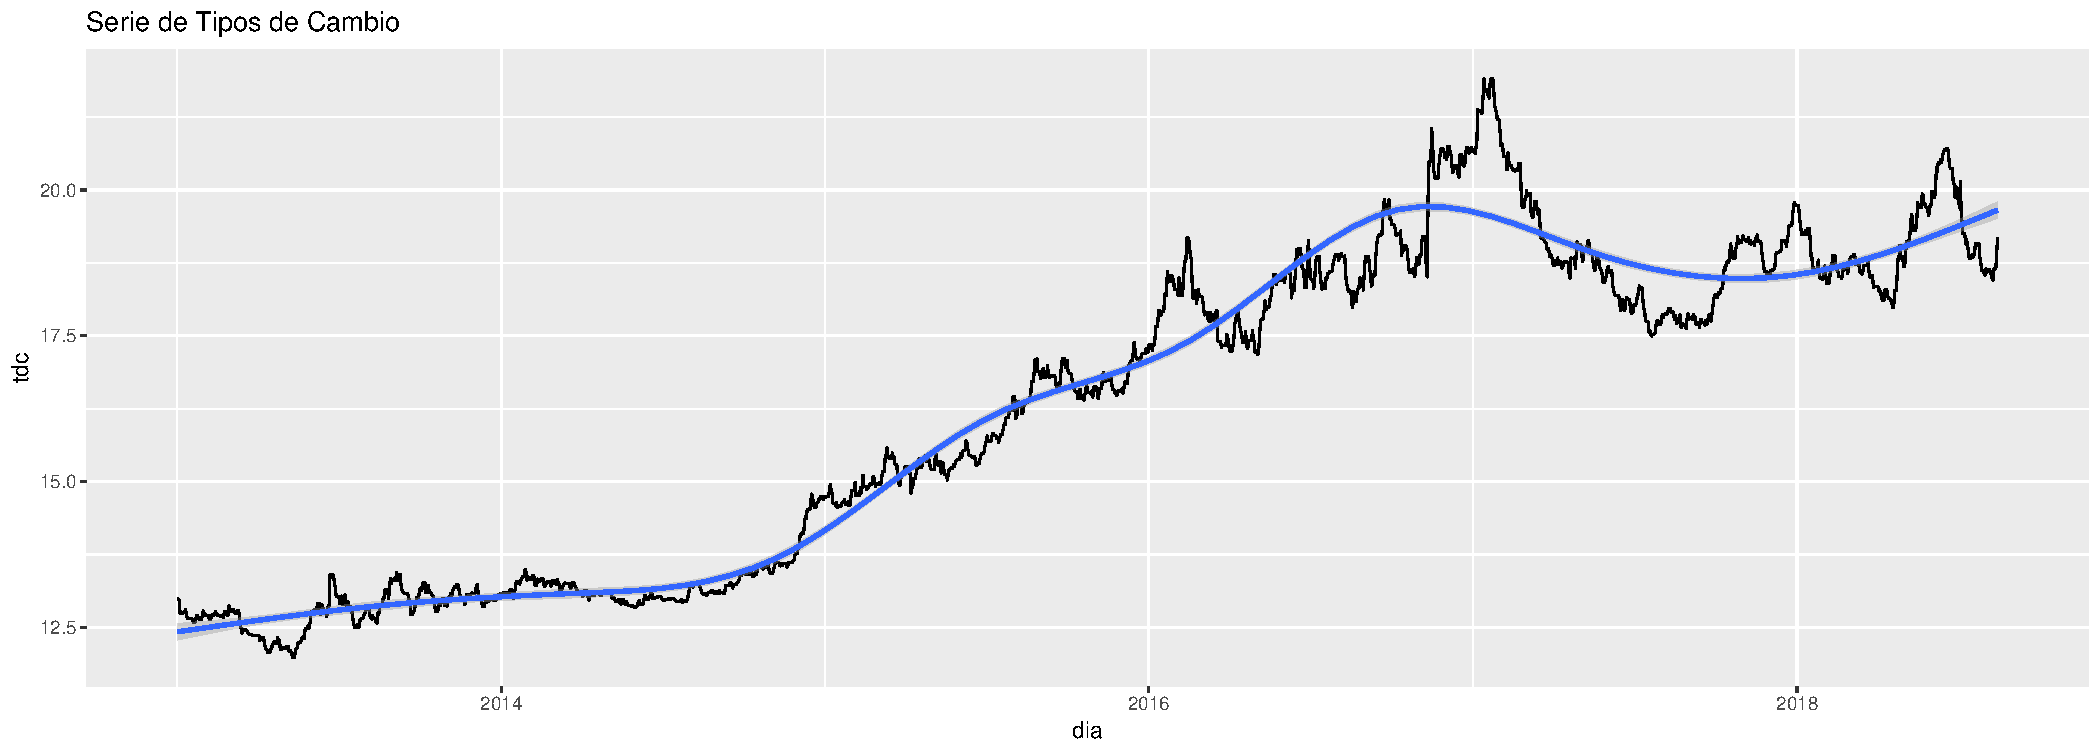
\includegraphics[width=\maxwidth]{figures/TiposdeCambio-1} 

\end{knitrout}
\paragraph{Correlación de variables}~\\
Para concluír el análisis exploratorio de datos estudiaremos la correlación de cada una de las variables contra el nível de ocupación, esto nos ayudará a decidir qué variables debemos utilizar dentro del modelo construído.
~\\
\begin{knitrout}
\definecolor{shadecolor}{rgb}{0.969, 0.969, 0.969}\color{fgcolor}
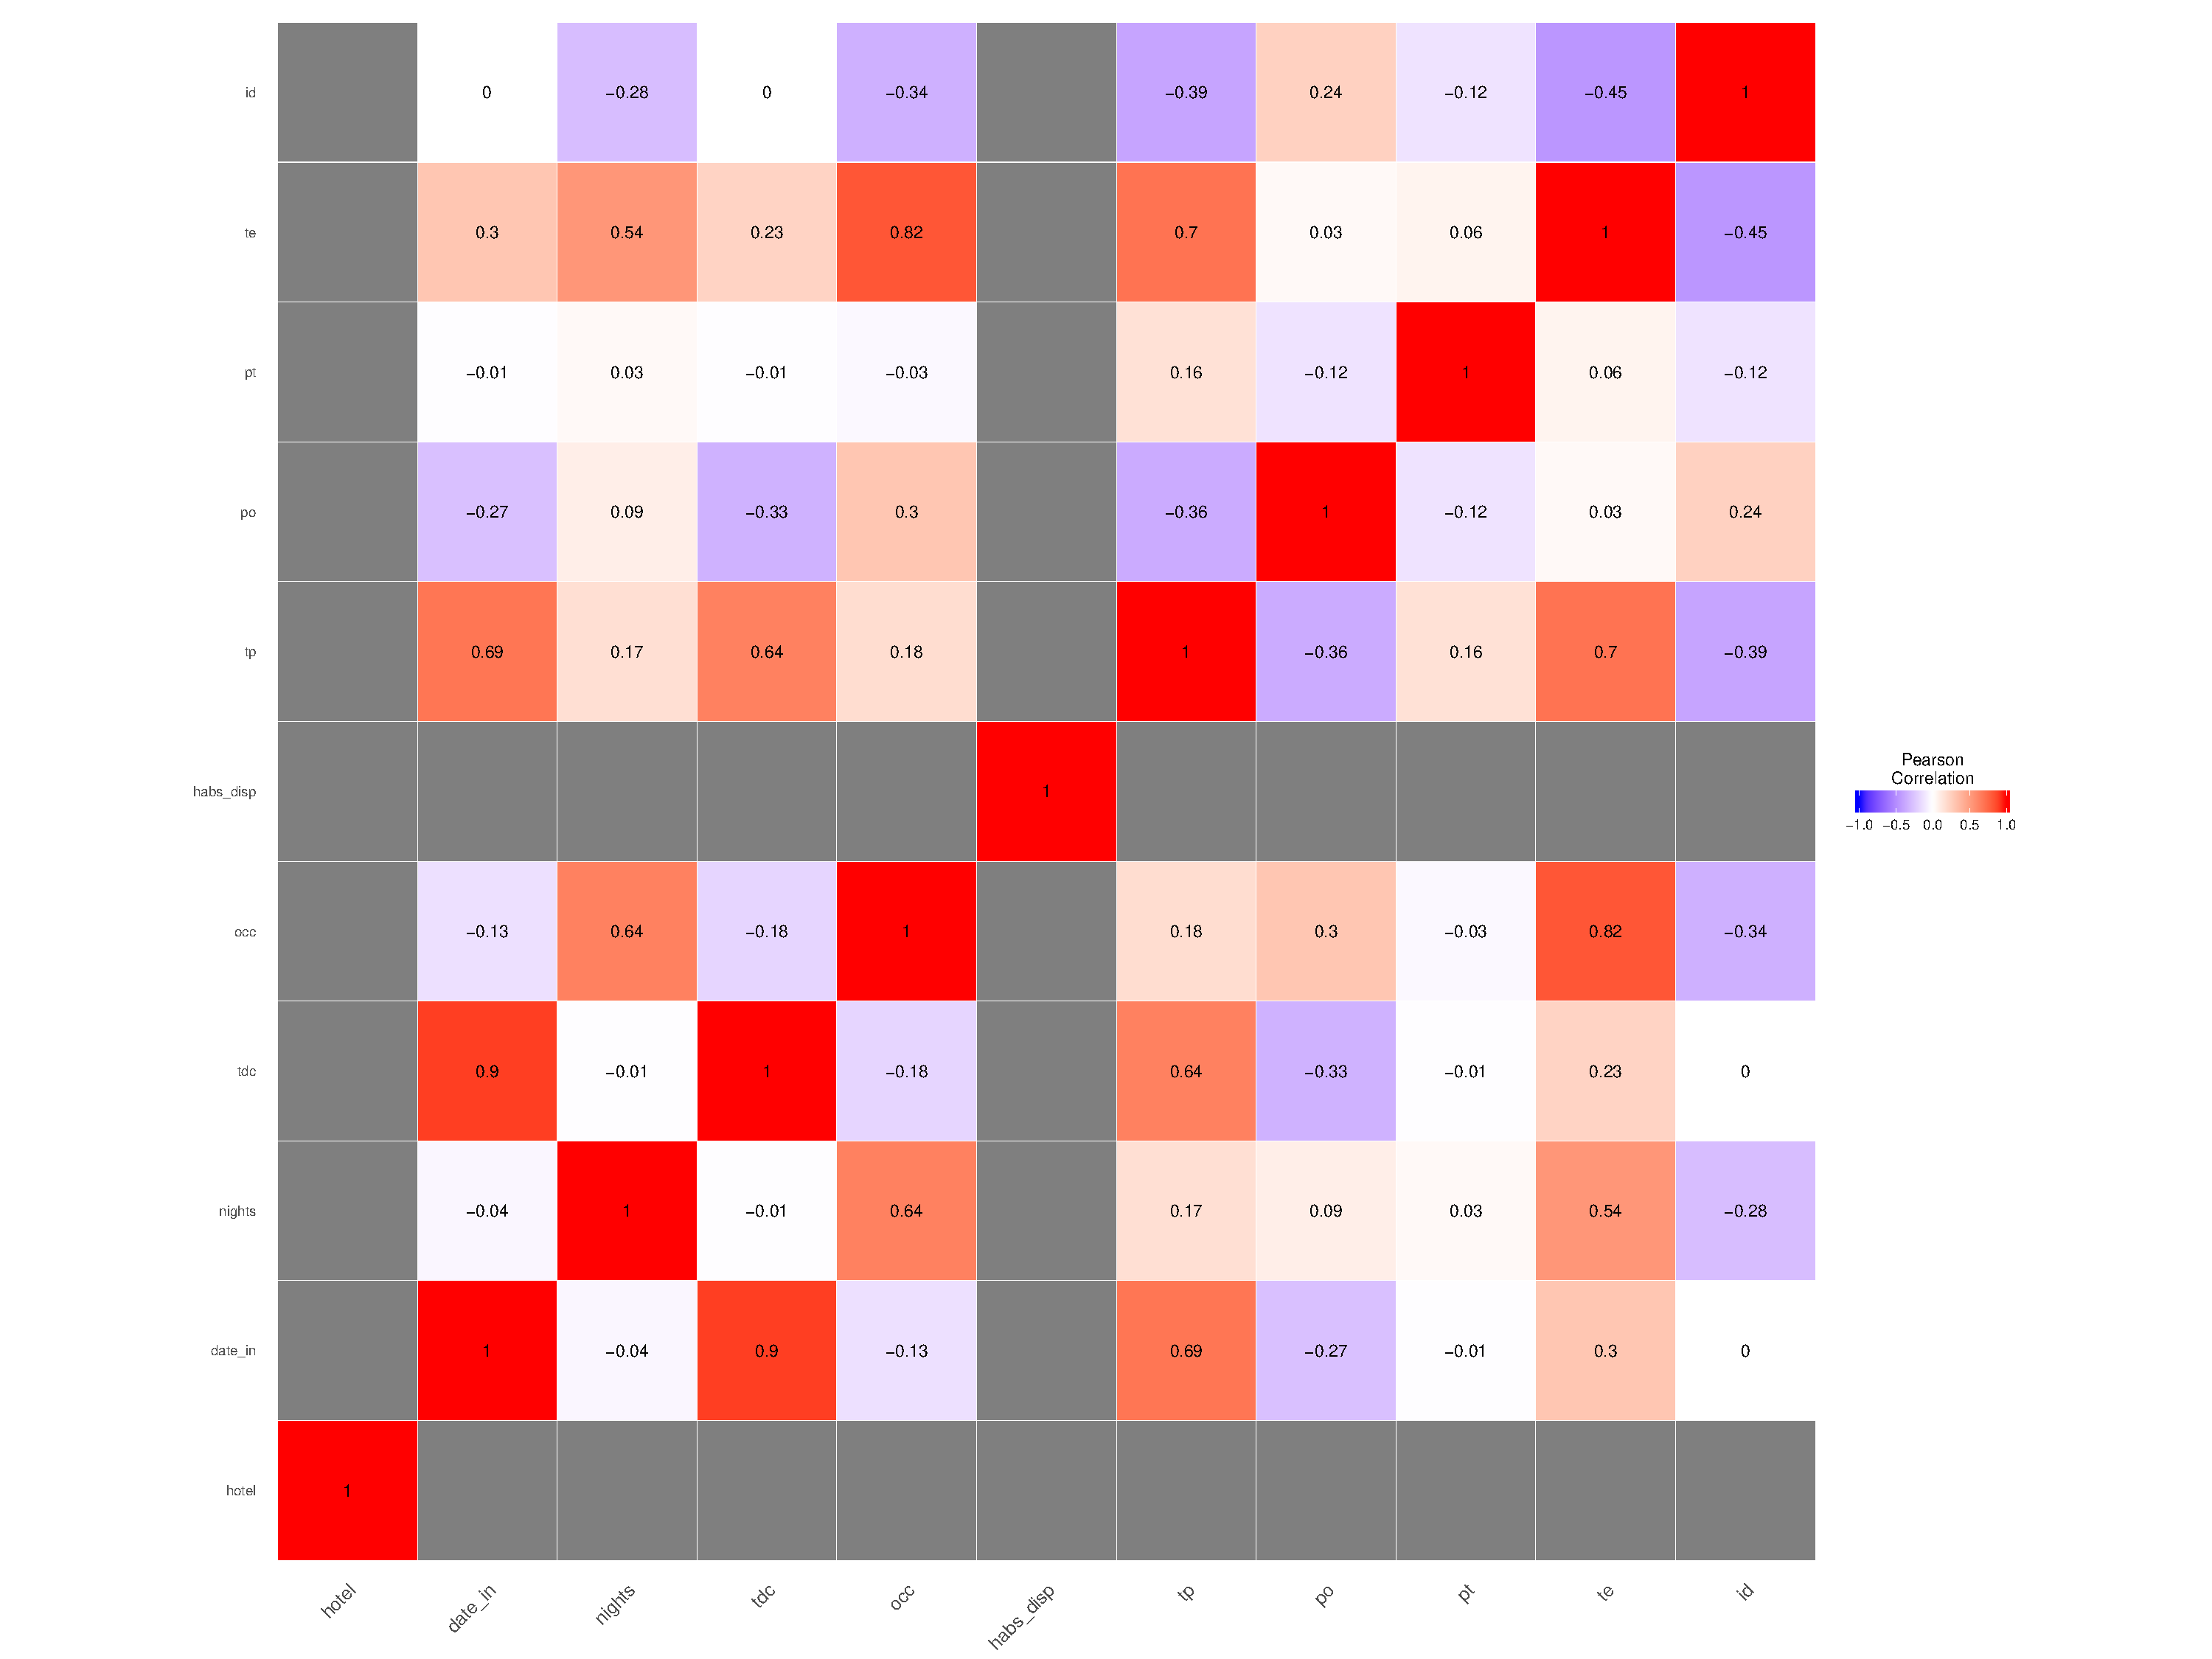
\includegraphics[width=\maxwidth]{figures/Correlacion-1} 

\end{knitrout}
~\\
\paragraph{Duración de Estancia}~\\
\begin{knitrout}
\definecolor{shadecolor}{rgb}{0.969, 0.969, 0.969}\color{fgcolor}
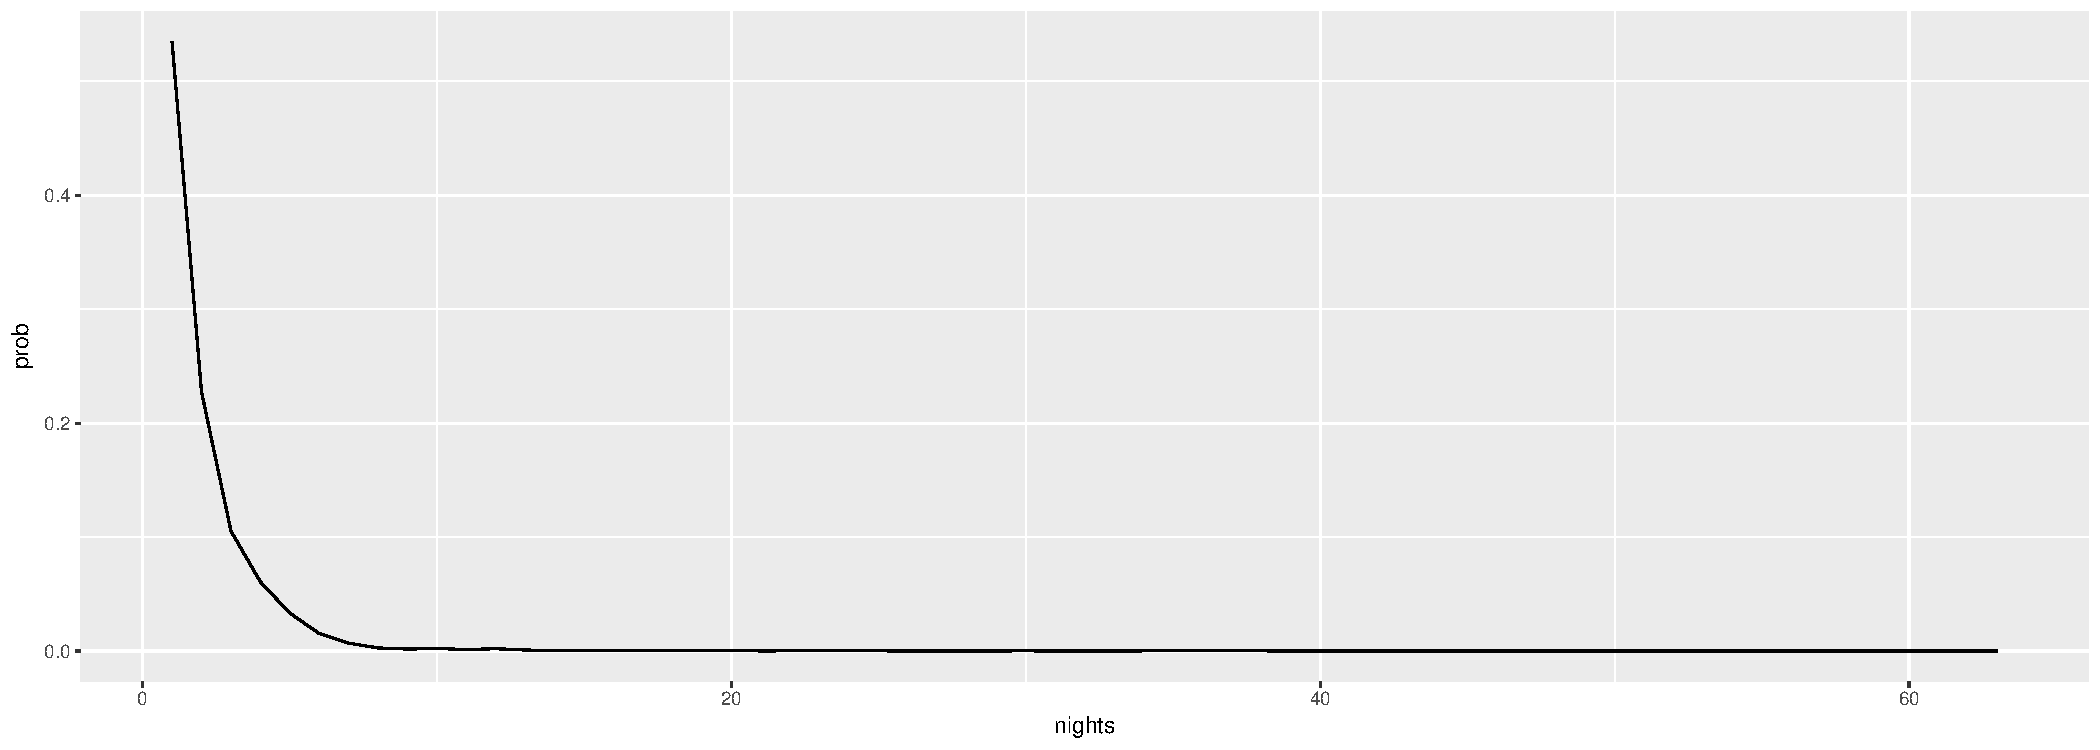
\includegraphics[width=\maxwidth]{figures/LOS1-1} 

\end{knitrout}
~\\
Podemos ver que la longitud de estancia se concentra entre 0 y 10 noches, por lo tanto estudiaremos este intervalo de cerca
~\\
\begin{knitrout}
\definecolor{shadecolor}{rgb}{0.969, 0.969, 0.969}\color{fgcolor}
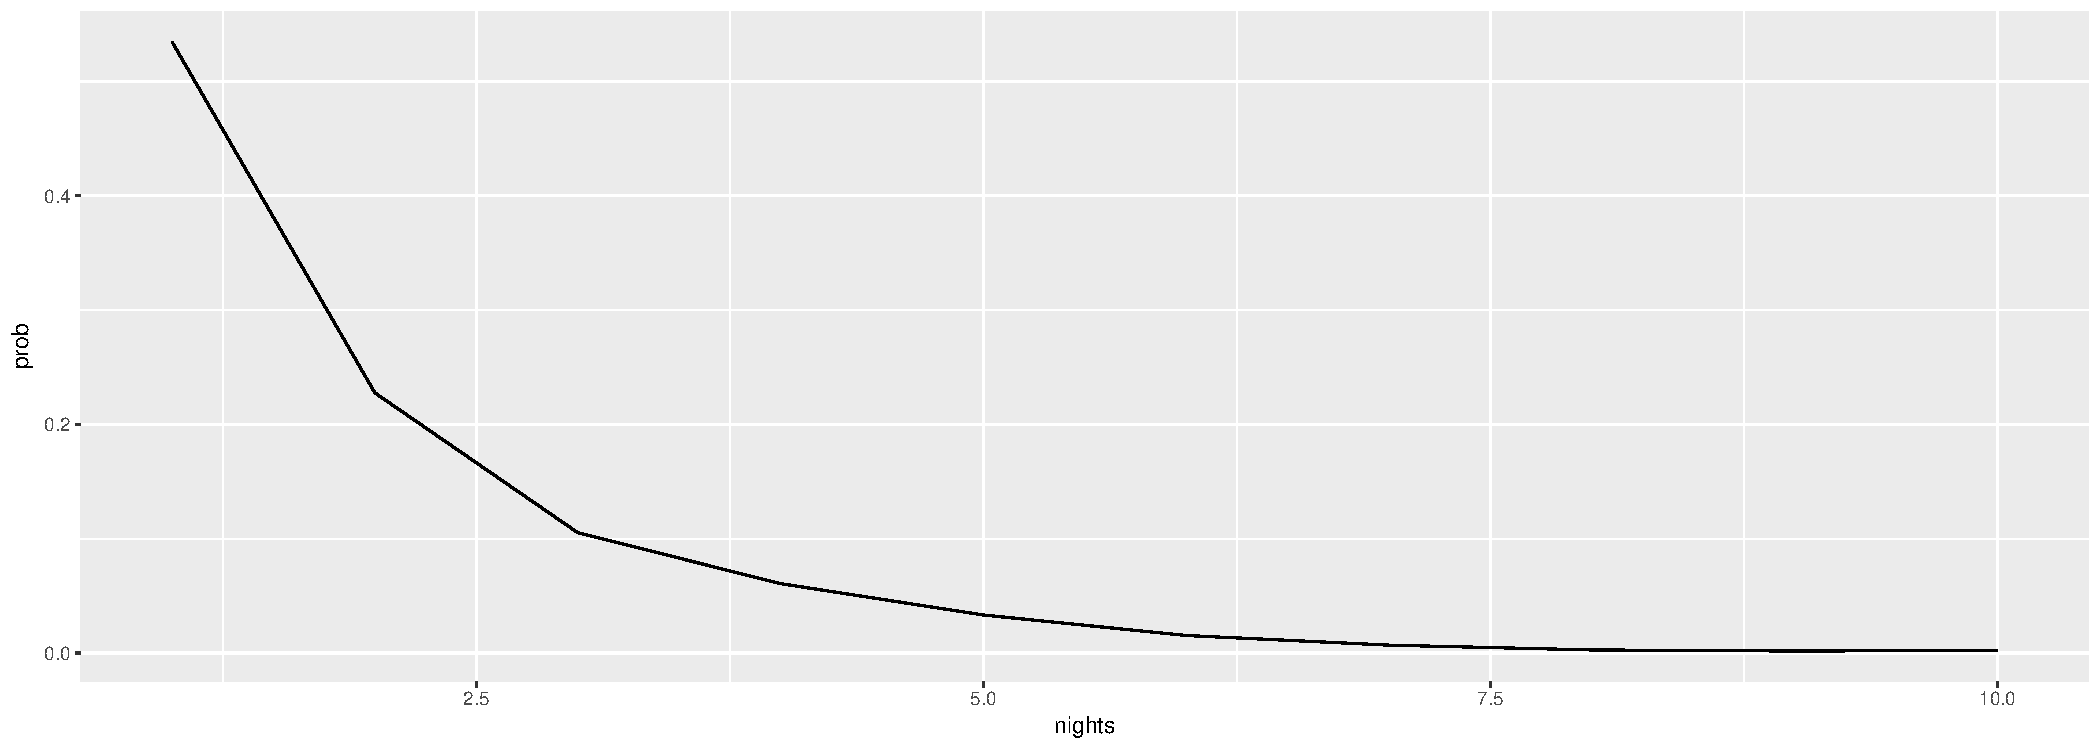
\includegraphics[width=\maxwidth]{figures/LOS2-1} 

\end{knitrout}
~\\

Derivado de este análisis podemos concluir lo siguiente:
\paragraph{Conclusiones}

\subsection{Propuesta de Modelo Predictivo}
\paragraph{Antecedentes del modelo} ~\\
Se le ha llamado "yield management" a la estrategia de variar precios basándose en el entendimiento, anticipación e influenciando el comportamiento de los clientes con el fin de poder maximizar el ingreso o utilidad generada por la venta de un inventario fijo de productos perecederos o que tienen un tiempo de venta limitado (como asientos en un vuelo o cuartos de hotel). La estrategia de "yield management involucra una estrategia de control de inventario para vender el producto correcto al cliente correcto en el tiempo correcto por un precio correcto. Dicho proceso puede resultar en una discriminación de precio, en la cual clientes consumiendo el mismo producto o servicio pagan precios totalmente diferentes. 
~\\
Para poder aplicar el concepto de "yield management" necesitamos que se den tres condiciones:
\begin{itemize}[noitemsep]
\item Debe existir un inventario fijo disponible para la venta.
\item Los productos deben de ser perecederos (o deben contar con un tiempo limite de venta. Una vez transcurrido este tiempo el producto pierde su valor).
\item Diferentes clientes están dispuestos a pagar diferentes precios por el mismo producto.
\end{itemize}
~\\
Las estrategias de "yield management" han alterado la industria del transporte y hospitalidad desde los años 80's. Desde el momento en el que estas estrategias fueron concebidas, estas empresas han requerido contar con analistas con un conocimiento detallado del mercado asi como con sistemas computacionales avanzados en los cuales se implementan sofisticados técnicas matemáticas que analizan el comportamiento del mercado y capturan oportunidades de ingresos.
~\\
\paragraph{Yield Management en la hotelería}~\\
En el caso de uso específico para la hotelería podemos estudiar la venta de habitaciones como la venta de un inventario fijo (dificilmente se puede incrementar o cambiar), que además las habitaciones que no se venden cada noche dejarán de producir ingresos a la propiedad por lo que se puede decir que caducaron. Es por ello que algunos hoteles utilizan software especializado para monitorear como es que los cuartos están siendo vendidos y reaccionar con base en sus observaciones. Hay varios métodos de control del inventario por ejemplo, ofrecer descuentos en propiedades con baja demanda o caso contrario, aumentar precios en propiedades con alta demanda. Otra forma de controlar el inventario es mediante la venta anticipada, es decir, se reserva parte del inventario para la venta anticipada a 30 días, 15 días, 7 días y un día y conforme se van agotando los cuartos los precios van cambiando, de tal forma que si pocos cuartos de una categoría han sido reservados, los precios para esa categoría bajan.
~\\
\paragraph{Trabajo previo}~\\
Existe una gran cantidad de literatura que describe trabajos realizados previamente con el objetivo de construír un modelo que pronostique la demanda de un producto y a partir de este pronóstico se fije un precio que maximize el ingreso del inventario.
~\\
Para la construcción de este modelo se revisaron artículos disponibles así como trabajos previos en esta área y se obtuvieron las siguientes conclusiones:
\begin{itemize}[noitemsep]
\item La mayoría de los modelos construídos anteriormente parten el problema de pricing en dos:
\subitem Modelo de pronóstico de demanda
\subitem Modelo de pricing dinámico
\item La mayoría de los artículos utilizan una simulación de montecarlo para simular la ocupación a futuro de las propiedades
\item Se debe estudiar cuidadosamente la temporalidad de la ocupación en el hotel
\item Se pueden utilizar factores multiplicadores que dependen de una serie de variables para poder asignar el nuevo precio del producto.
\item La demanda de la propiedad (en el caso de hoteles) puede ser modelada como un proceso poisson.
\item Se pueden incluír heurísticas de control de inventario, aunque esto tiende a complicar el modelado.
\item El precio dependerá también del inventario que aún está disponible en cualquier momento en el que se dé una reservación.
\end{itemize}
~\\
Tomamos estas conclusiones como punto de partida para el modelo realizado en CityExpress.

\paragraph{Descripción del modelo} ~\\
Para el desarrollo del modelo utilizaremos los data sets que contienen la información de las reservaciones modelados como curvas de "pick up". Estas curvas nos describen la velocidad en que un hotel vende su inventario para un día en específico. Lo que el modelo hará es ajustar una curva que resuma el comportamiento del hotel para un día similar al que se está estudiando, de esa manera podremos predecir cuantos cuartos venderá el hotel y con cuantos días de antelación.Para lograr esto se construirá un modelo de regresión Poisson fundamentado en la distribución de la llegada de las reservaciones como un proceso discreto que depende del tiempo y para darle un enfoque de uso predictivo al modelo, se utiliza un modelo de regresión lineal con predictores que dependen del tiempo para dar un valor estimado por día y por hotel de las curvas de "pick Up".
\paragraph{Modelo de regresión Poisson} ~\\
Por la naturaleza del estudio que se está realizando se optó por implementar una regresión Poisson, la cuál es un modelo linear genearlizado usado comúnmente en problemas de conteos de datos y tablas de contingencia. La regresión de Poisson asume que la variable de respuesta $Y$ tiene una distribución de Poisson y también asume que el logaritmo de su valor esperado puede ser modelado por una comibinación lineal de los parámetros desconocidos.
El modelo de regresión Poisson puede ser expresado como sigue:
$$\log(E(Y|X))=\beta_0 + \beta_1{X}$$
Para poder aplicar el modelo a la información proporcionada, se contruyeron series por día y hotel en función del número de días de antelación para la reservación.
~\\
La selección del modelo de regresión Poisson se fundamenta en la distribución de la llegada de las reservaciones como un proceso discreto que depende del tiempo. El conteo de las reservaciones es inversamente proporcional a la cercanía de la fecha de entrada al hotel y por tanto la probabilidad de ocurrencia de llenado del hotel incrementa conforme se acerca la fecha para la que se hace la reservación.

\paragraph{Modelo de regresión lineal} ~\\
Considerando que las principales variables que describen la predictividad de la demanda son temporales, se propone un modelo que explique los parámetros de las curvas de "pick up" mediante un modelo lineal. Se generan series temporales para hacer predictivo el modelo de pronóstico de demanda y proyectamos en función de la historia en el mismo día calendario del año anterior, el día de la semana para compensar los efectos diferenciados por hotel, así como los eventos que afectan la demanda en un calendario anticipado por hotel, y finalmente el comportamiento de las tarifas que ofrece la competencia.
$$\log(E(Y|X))=\beta_0 + \beta_1{X}$$
\subsection{Interpretación del modelo}
El modelo genera como resultado un data set similar al que se muestra a continuación:
~\\
\begin{knitrout}
\definecolor{shadecolor}{rgb}{0.969, 0.969, 0.969}\color{fgcolor}\begin{kframe}
\begin{verbatim}
##   hotel        dia  AAbeta0       AAbeta1 AAvariacion
## 1 CEINS 2018-01-01 2.335294 -2.489863e-06   0.1884625
## 2 CEINS 2018-01-02 2.984073 -2.818019e-06   0.1321997
## 3 CEINS 2018-01-03 3.301841 -3.535574e-06   0.3262416
## 4 CEINS 2018-01-04 3.782523 -2.295688e-06   0.1744051
## 5 CEINS 2018-01-05 3.761697 -1.089675e-06   0.0925871
## 6 CEINS 2018-01-06 3.140137 -2.292639e-06   0.1887511
##       tdc       PO       PT    diasem  mes eventos1 eventos
## 1 19.7354 0.840382 0.872720     lunes ene.        0       0
## 2 19.7354 1.096970 1.025310    martes ene.        0       0
## 3 19.6629 0.927171 0.992081 miércoles ene.        0       0
## 4 19.4899 1.045640 1.024860    jueves ene.        0       0
## 5 19.3717 0.927771 0.953648   viernes ene.        0       0
## 6 19.2427 1.334990 0.908828    sábado ene.        0       0
##   pred.beta0  pred.beta1
## 1   3.159533 -0.12278602
## 2   3.916035 -0.11603131
## 3   3.874017 -0.10891126
## 4   4.159721 -0.10283409
## 5   3.698266 -0.08467446
## 6   3.771660 -0.09371103
\end{verbatim}
\end{kframe}
\end{knitrout}
~\\
Las variables de interés son: "pred.beta0" y "pred.beta1" ya que son los parámetros generados por los modelos y que nos ayudarán a reconstruír las curvas de pickup. Para reconstruír la curva de pickup de un día en específico, debemos obtener los parámetros "pred.beta0" y "pred.beta1" para el día elegido y posteriormente debemos calcular hacer el siguiente cálculo: $$E[y|x]=e^{\beta_0 + \beta_1{x}}$$
~\\
Dónde:
\begin{itemize}[noitemsep]
\item $E[y|x]$ = El valor esperado de cuartos noches para un día en específico
\item $\beta_0$ = pred.beta0
\item $\beta_1$ = pred.beta1
\item $x$ = días de antelación al día analizado
\end{itemize}
~\\
Validamos el modelo con fechas aleatorias y obtenemos las siguientes gráficas:
~\\
\begin{knitrout}
\definecolor{shadecolor}{rgb}{0.969, 0.969, 0.969}\color{fgcolor}
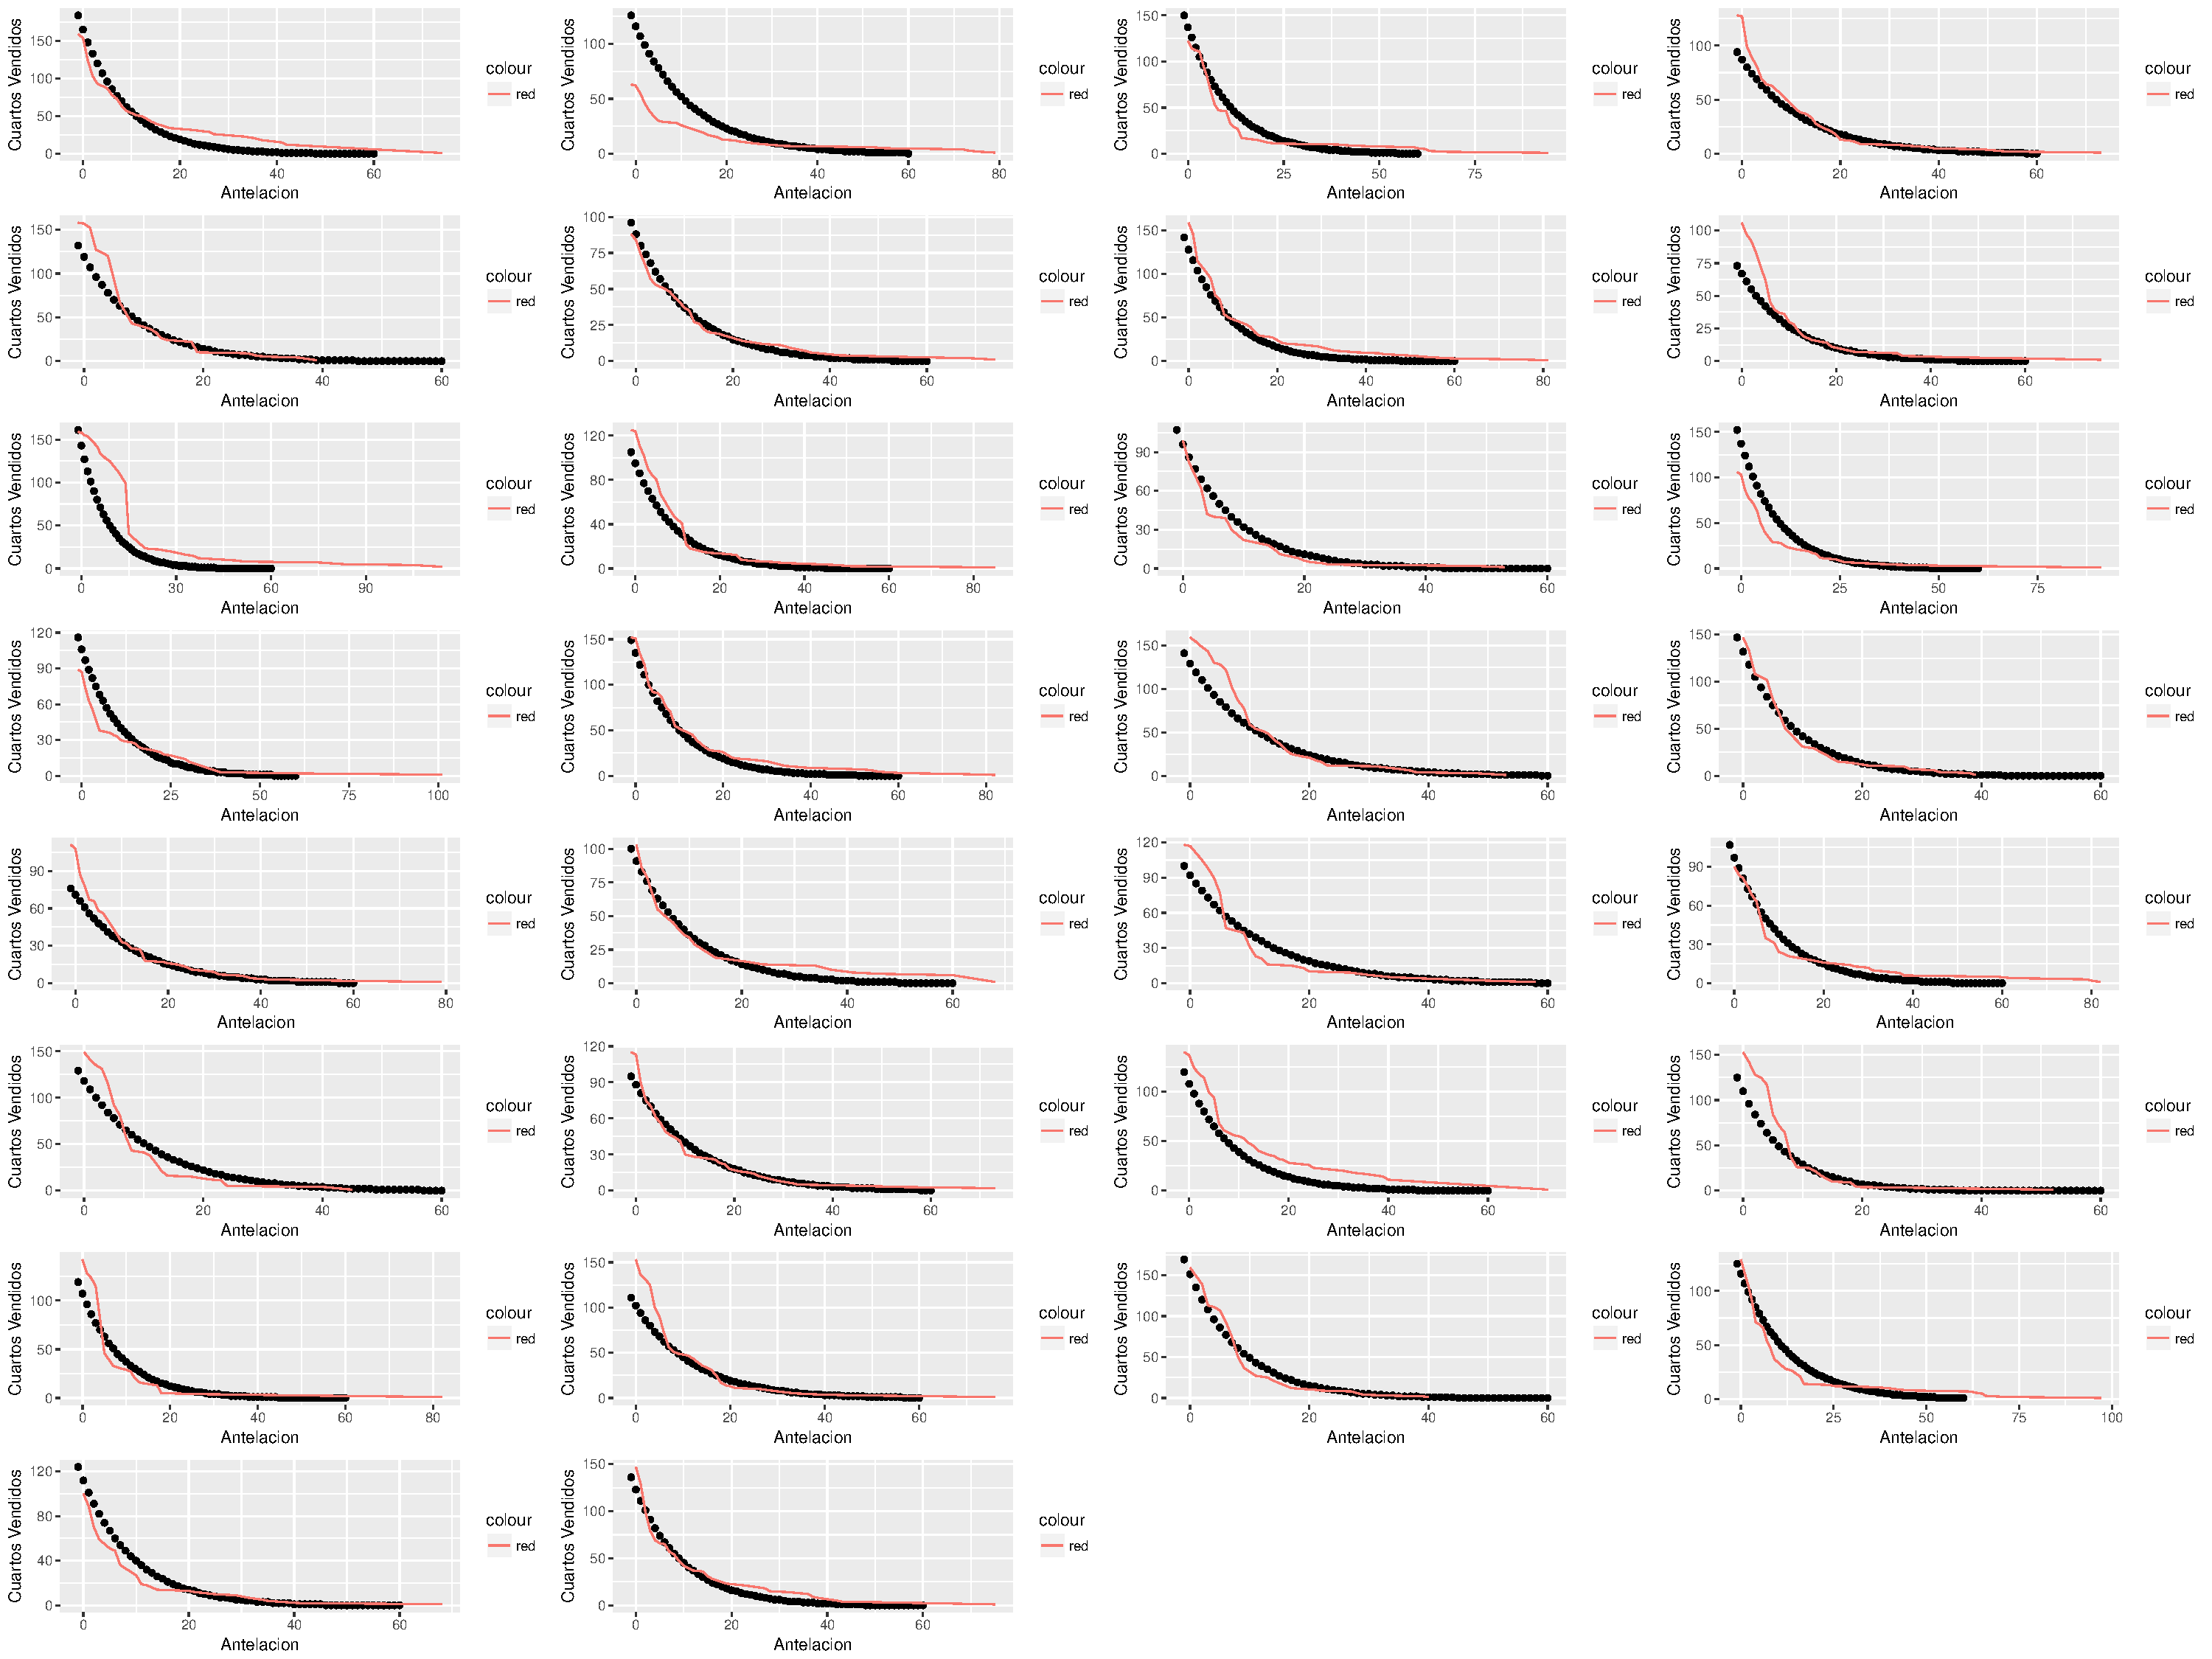
\includegraphics[width=\maxwidth]{figures/ValidacionModelo-1} 

\end{knitrout}

\begin{knitrout}
\definecolor{shadecolor}{rgb}{0.969, 0.969, 0.969}\color{fgcolor}\begin{kframe}


{\ttfamily\noindent\bfseries\color{errorcolor}{\#\# Error in detach(package:plyr): invalid 'name' argument}}\begin{verbatim}
## [1] "mape:"
## [1] 17.67243
\end{verbatim}
\end{kframe}
\end{knitrout}
~\\
\paragraph{Modelo simple de pricing dinámico}~\\
Una vez pronósticado el nível de ocupación para cada una de las propiedades de la cadena, se alimentó un modelo de pricing dinámico que entrega recomendaciones de precios para la tarifa pública tomando en cuenta la demanda pronósticada para cierto día del año.

~\\
\subparagraph{Problema de asignación de precios}~\\
Típicamente el gerente de la propiedad controla la cantidad de cuartos ofrecidos a diferentes precios, es decir, se asigna cierto número de cuartos a cada nível de tarifa de tal forma que cuando el inventario asignado al precio mas bajo se agota, se consume el inventario asignado al siguiente nivel de tarifa que será mayor al primer precio ofertado. 
~\\
A continuación se muestra un esquema donde se ejemplifica la idea mencionada anteriormente:

\begin{figure}[!]
  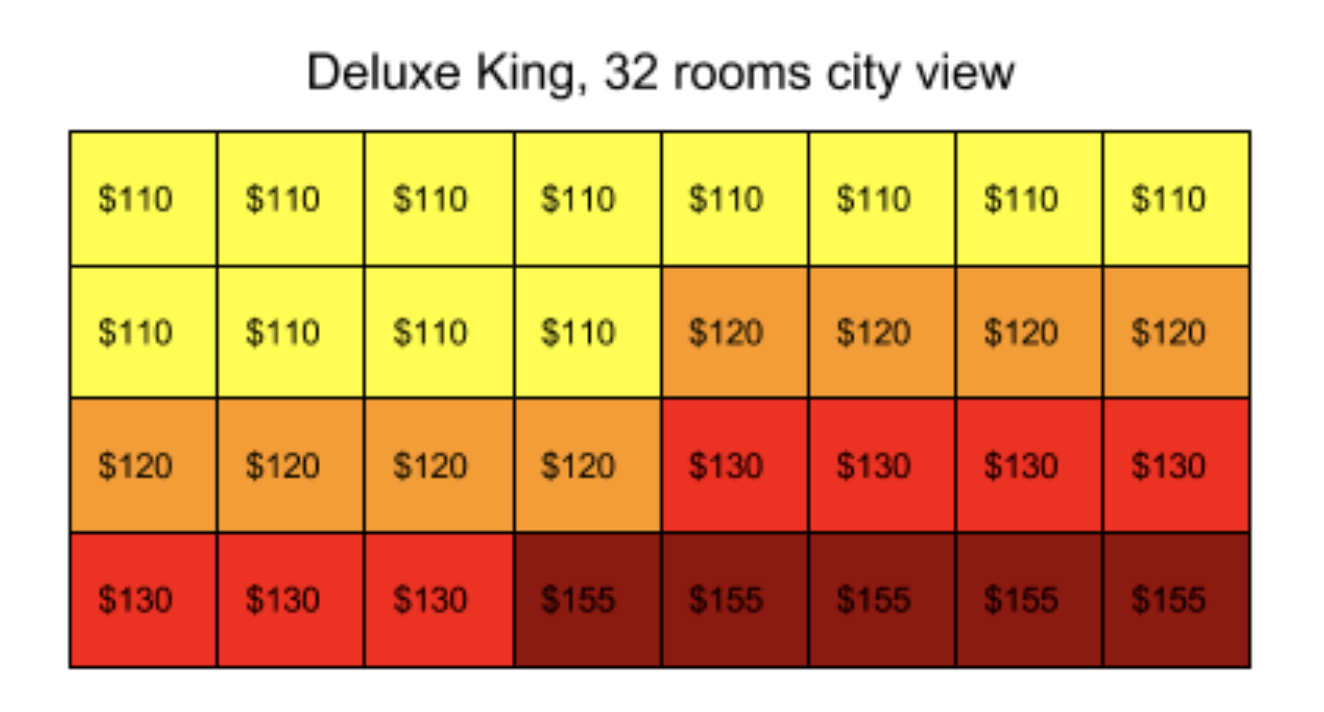
\includegraphics[width=\linewidth]{Imagenes/buckets.png}
  \caption{Asignacion de inventario}
  \label{fig:Asignacion de Inventario}
\end{figure}

~\\
Como se puede observar, tenemos un inventario de 32 cuartos divido en 4 níveles de precios:
\begin{itemize}[noitemsep]
\item 12 cuartos son ofrecidos a un valor de 110 USD
\item 8 cuartos son ofrecidos a un valor de 120 USD
\item 7 cuartos son ofrecidos a un valor de 130 USD
\item 5 cuartos son ofrecidos a un valor de 155 USD
\end{itemize}
~\\
Hay que considerar que el hecho de poder encontrar el precio que maximiza el ingreso de una propiedad constituye un problema complejo de optimización, en donde el hotel debería explorar un gran número de escenarios, sin embargo, para superar la complejidad computacional que este calculo requiere muchos hoteles han optado por usar varias simplificaciones por ejemplo, utilizar un enfoque basado en la asignación de precios, en la cual se pre asigna un número fijo de inventario disponible a cada nível de precios y los precios pueden variar a lo largo del tiempo.
~\\
\subparagraph{Formulación Matemática}~\\
Un problema de maximización de ingresos es básicamente un problema de optimización sujeto a restricciones, en este caso, se quiere maximizar la siguiente función objetivo:
$$\sum_{n=0}^{n}p_i*o_i$$
En donde i es la índice de la noche, $p_i$ es el precio del cuarto para la i-ésima noche y $o_i$ es la ocupación pronósticada (demanda) para la i-ésima noche al precio $p_i$. Asumimos también que la función de la ocupación (demanda) está sujeta al precio bajo la siguiente relación:
$$o = o_{nominal} * (\frac{p}{p_{nominal}})^e$$
Donde $o_{nominal}$ corresponde a la ocupación pronosticada para una noche dada tomando como base un precio nominal ($p_{nominal}$). Para este caso el $p_{nominal}$ es igual a la tarifa pública promediada a lo largo del año. El valor de $e$ (elasticidad) toma un valor = -2. En otras palabras, $p$ incrementa en un 10\% y la demanda decrece cerca de un 20\%.
~\\
Para poder hacer una asignación dinámica de los precios, evitando tener que correr el modelo conforme la información del hotel es actualizada, se partió el inventario en 4 níveles de disponiblidad (159,120,80 y 40 cuartos disponibles). Para cada nível de capacidad se resolvió la función objetivo para obtener 4 conjuntos de precios, de esta forma, el gerente de la propiedad puede saber a qué nível de precio debe subir la tarifa pública de la propiedad conforme las habitaciones disponibles decrecen.
~\\
\subparagraph{Limitantes del modelo}~\\
Este modelo se formuló considerando los siguientes puntos:
\begin{itemize}[noitemsep]
  \item Se consideran estancias de una sola noche
  \item No se toman en cuenta reservaciones para grupos ni cancelaciones
  \item Asusmimos paridad de precios entre los canales, es decir, los precios no varían entre los canales de venta
  \item Se considera solamente un tipo de habitación, el incremento por cambio de habitación es un monto fijo conocido como gap
  \item Se asume un valor para la elasticidad (-2) que es un valor razonable para la industria
\end{itemize}


\subparagraph{Resultados del modelo de pricing}~\\
El modelo de pricing, como comentarmos anteriormente, arroja como resultado una matriz de día vs precio por niveles de inventario. A continuación se muestra un ejemplo:
~\\
\begin{knitrout}
\definecolor{shadecolor}{rgb}{0.969, 0.969, 0.969}\color{fgcolor}\begin{kframe}
\begin{verbatim}
##            day       40       80      120      159
## 107 2018-04-17 1797.715 2177.611 2052.235 1782.867
## 58  2018-02-27 1758.654 1935.701 1672.648 1453.103
## 144 2018-05-24 1792.407 2141.922 1985.174 1724.609
## 51  2018-02-20 1799.337 2188.696 2074.106 1801.868
## 67  2018-03-08 1780.087 2062.619 1851.891 1608.820
## 56  2018-02-25 1766.800 1982.328 1734.455 1506.798
## 203 2018-07-22 1761.104 1949.520 1690.537 1468.645
## 184 2018-07-03 1798.808 2185.047 2066.841 1795.557
## 187 2018-07-06 1752.048 1899.247 1627.063 1413.502
## 154 2018-06-03 1762.291 1956.279 1699.412 1476.355
## [1] 57555.7
\end{verbatim}
\end{kframe}
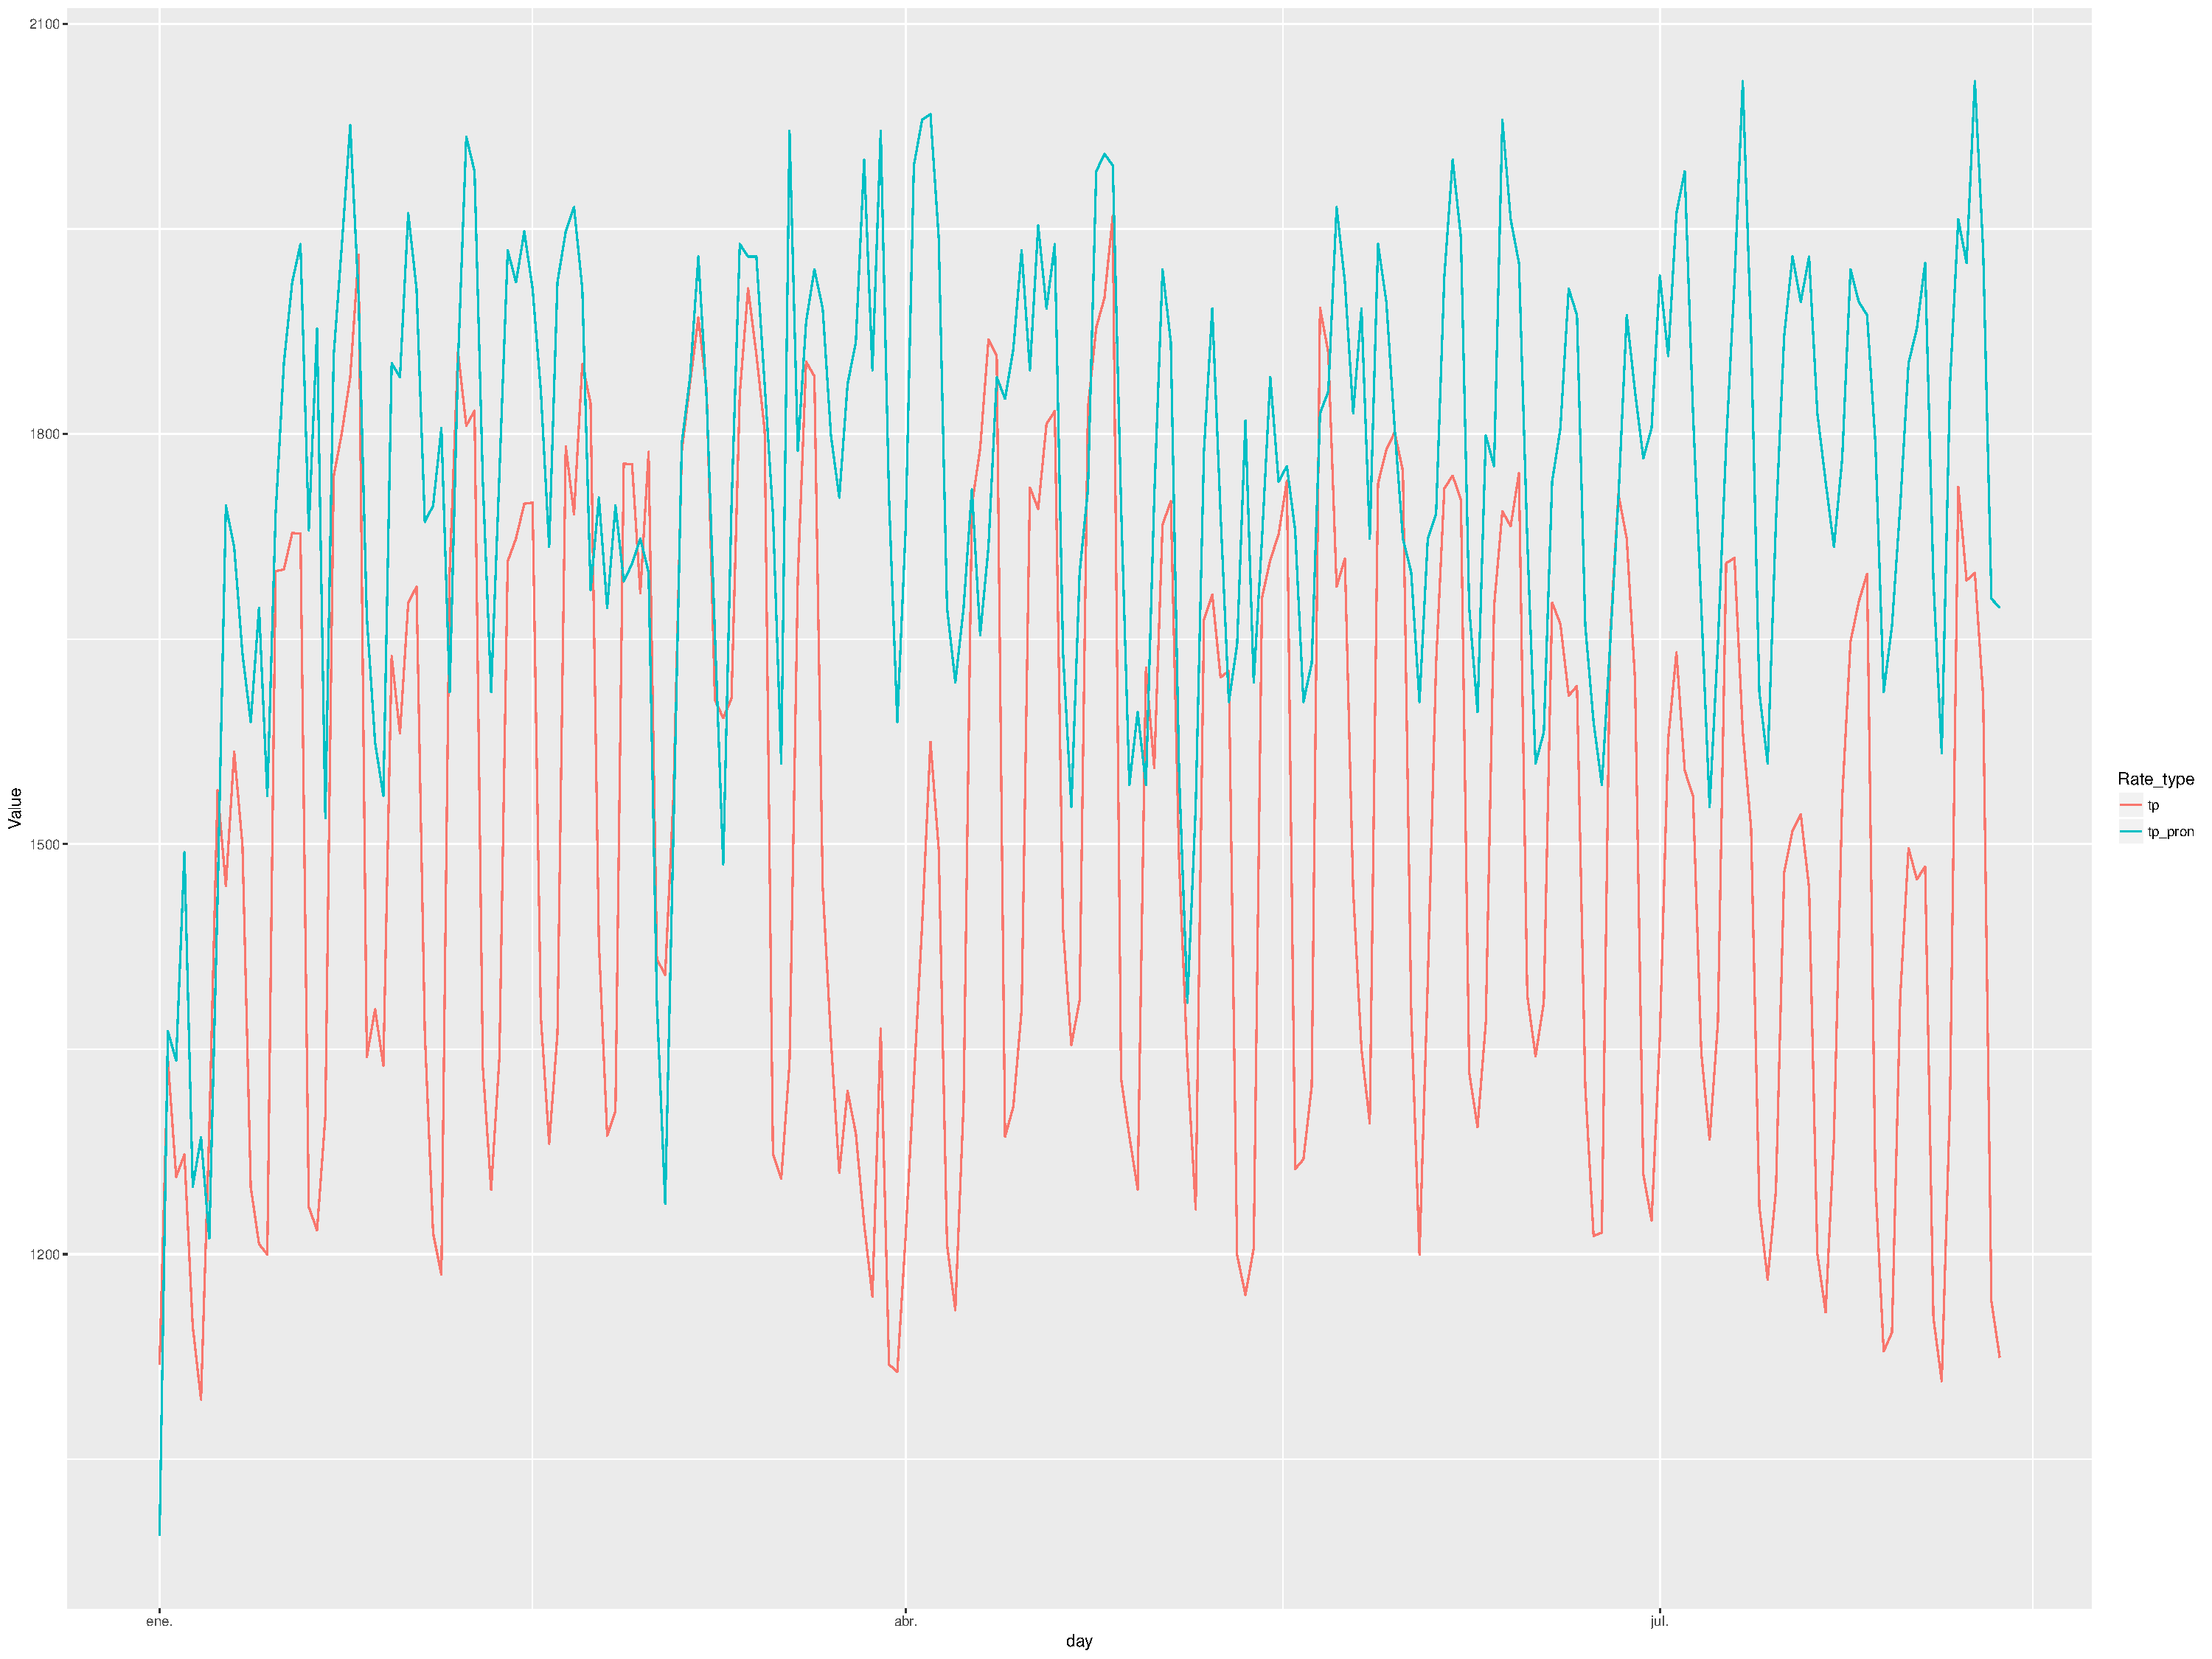
\includegraphics[width=\maxwidth]{figures/Pricing-1} 

\end{knitrout}
~\\
Graficando los resultados:
~\\
\begin{knitrout}
\definecolor{shadecolor}{rgb}{0.969, 0.969, 0.969}\color{fgcolor}\begin{kframe}
\begin{verbatim}
##          day       40       80       120       159
## 1 2018-01-01 1404.540 1017.112  831.8153  722.6349
## 2 2018-01-02 1658.592 1502.048 1226.4447 1065.4671
## 3 2018-01-03 1649.574 1471.733 1201.6655 1043.9403
## 4 2018-01-04 1705.934 1676.832 1387.5638 1205.4384
## 5 2018-01-05 1604.489 1343.501 1096.9655  952.9827
## 6 2018-01-06 1623.362 1392.960 1137.3580  988.0735
##     tp_pron      tp
## 1  994.0256 1119.21
## 2 1363.1380 1342.68
## 3 1341.7283 1256.69
## 4 1493.9420 1273.01
## 5 1249.4846 1147.34
## 6 1285.4382 1093.78
\end{verbatim}
\end{kframe}
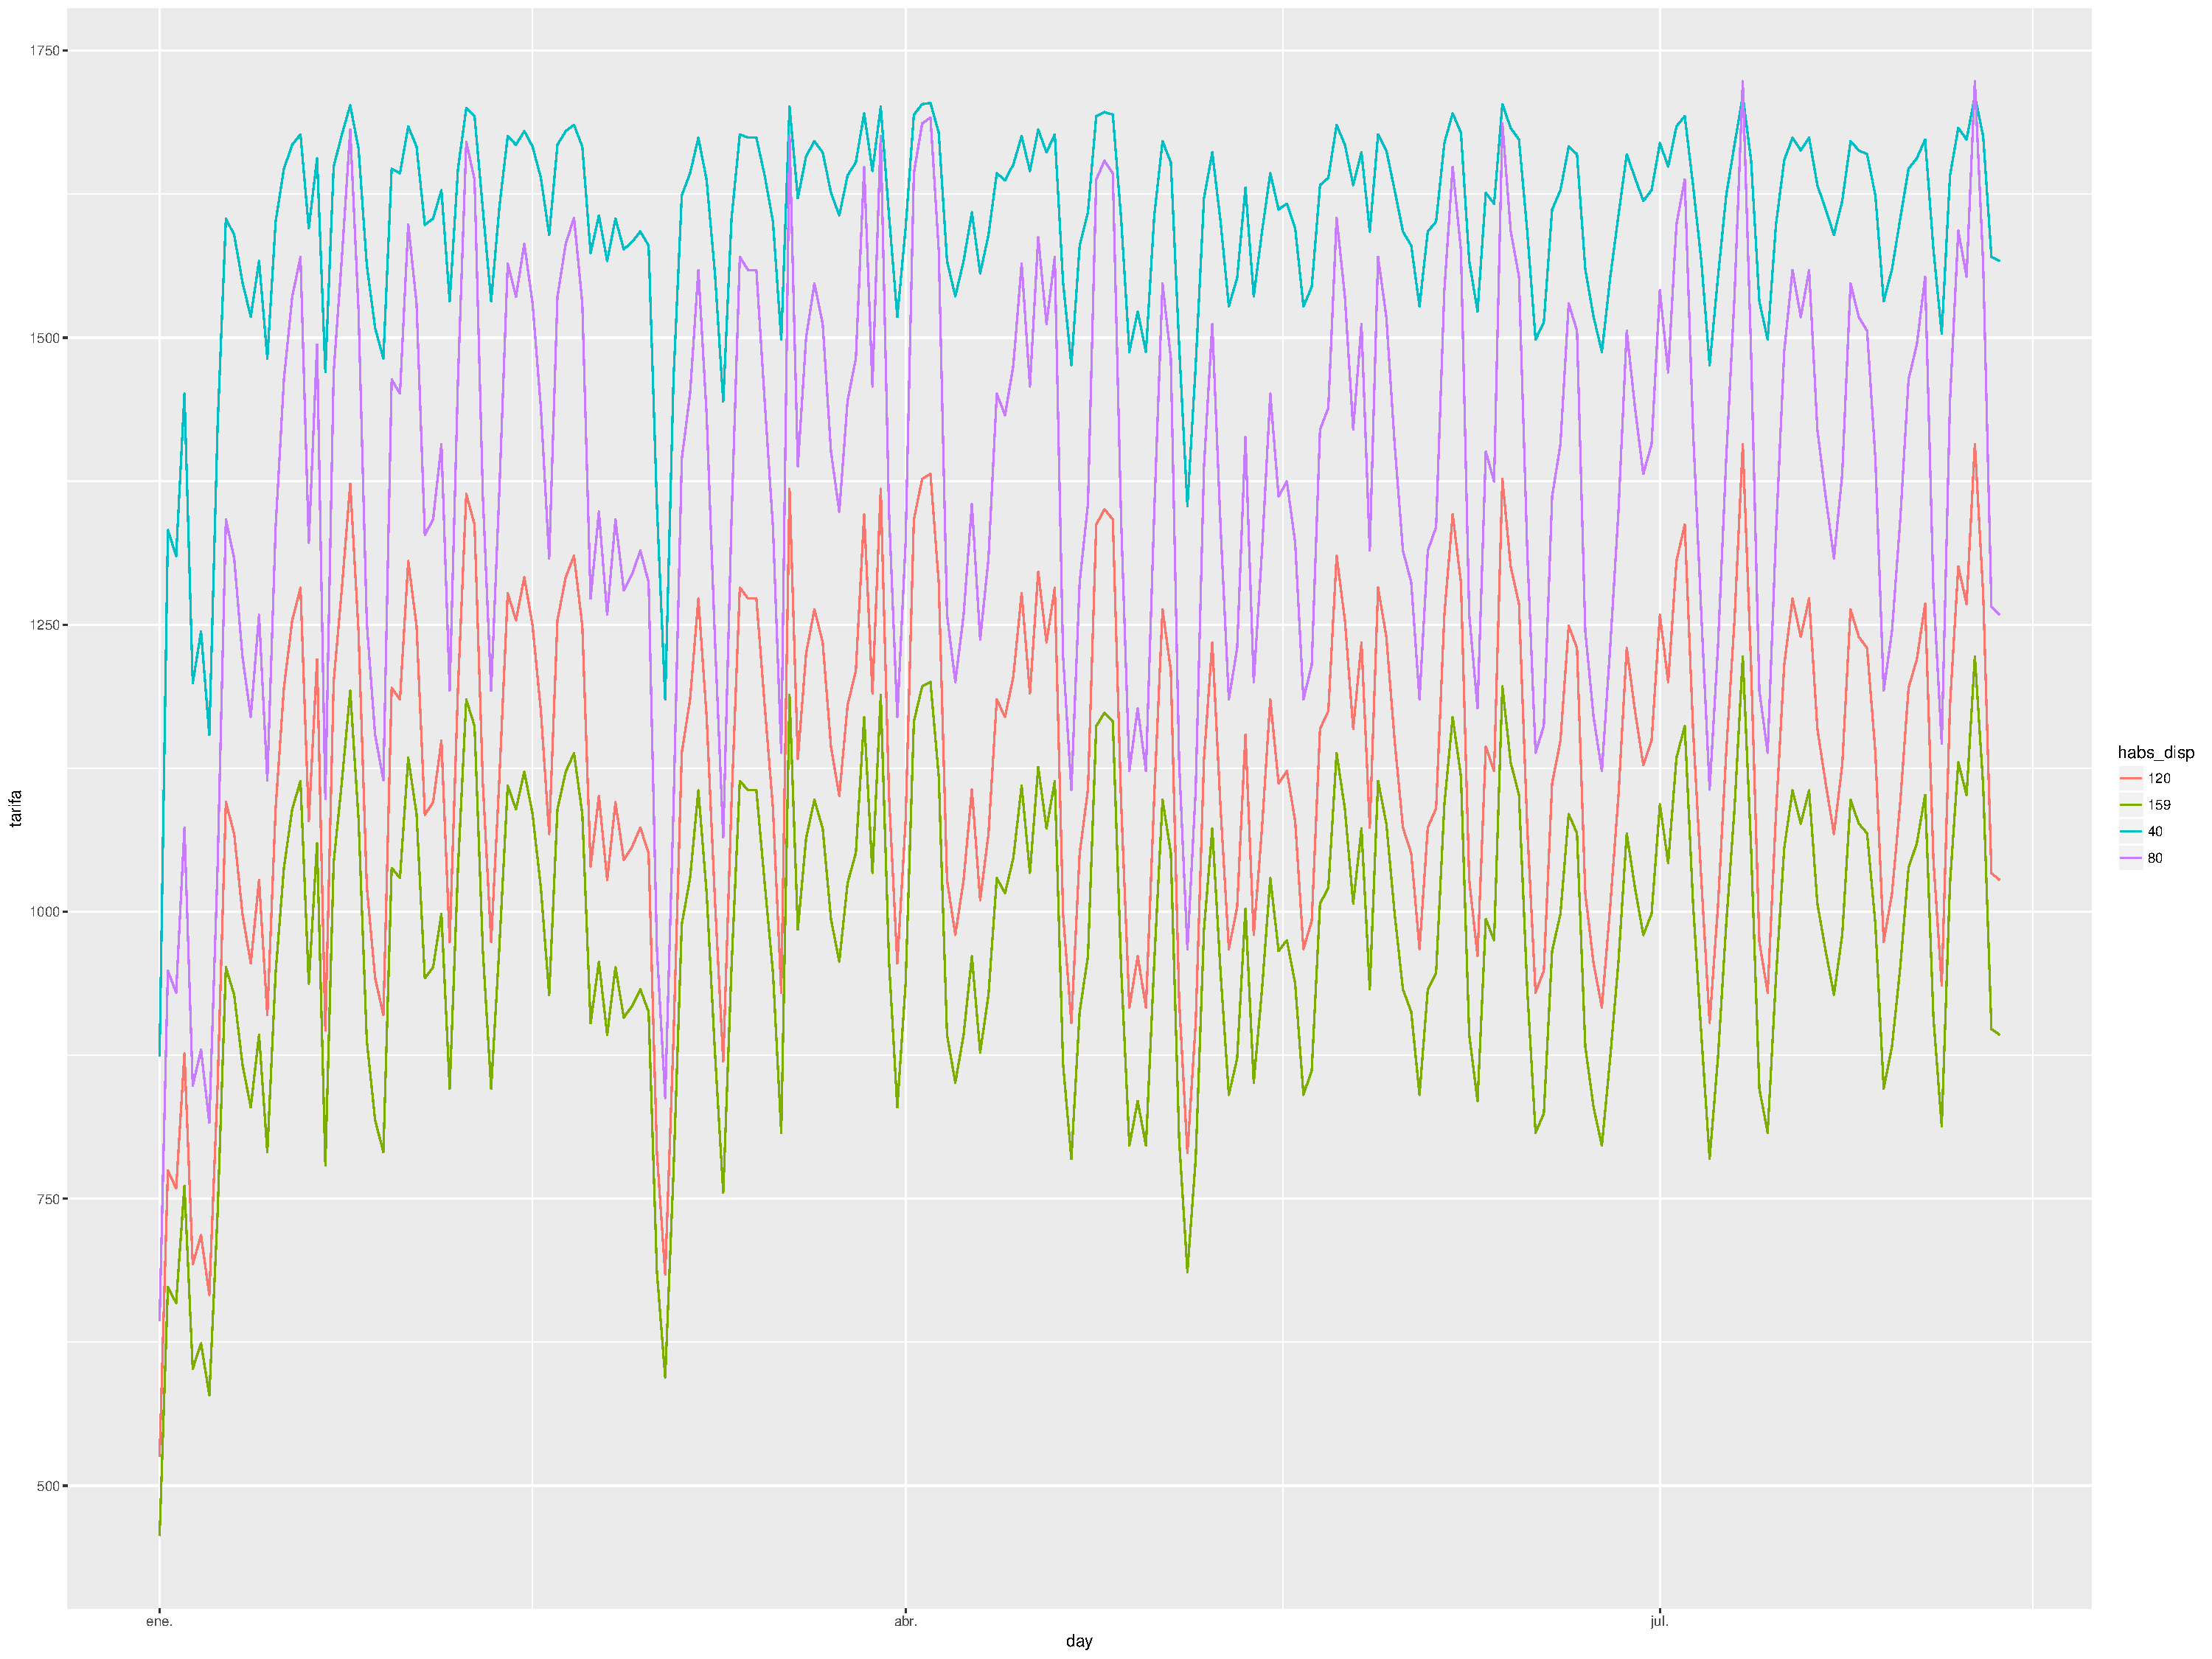
\includegraphics[width=\maxwidth]{figures/Pricing_graph-1} 

\end{knitrout}
\section{Anexo A: Implementación del modelo pronóstico de demanda}
\begin{knitrout}
\definecolor{shadecolor}{rgb}{0.969, 0.969, 0.969}\color{fgcolor}\begin{kframe}
\begin{alltt}
\hlkwd{library}\hlstd{(plyr)}
\hlstd{HIS_CEINS}\hlkwb{<-}\hlkwd{read_csv}\hlstd{(}\hlstr{"datos/EST_PAS_UNIC_CEINS.csv"}\hlstd{)}
\hlstd{RES_CEINS} \hlkwb{<-} \hlkwd{read.csv}\hlstd{(}\hlstr{"datos/CEINS_RESERVAS.csv"}\hlstd{)}
\hlcom{#Juntamos todas las tablas en un solo dataset}
\hlcom{#datos <- rbind(HIS_CEINS, RES_CEINS)}
\hlstd{datos} \hlkwb{<-} \hlstd{HIS_CEINS}
\hlcom{#Modelo de regresion Poisson para obtener}
\hlcom{#parametros de modelo predictivo}
\hlstd{modelo.1}\hlkwb{<-}\hlkwa{function}\hlstd{(}\hlkwc{base}\hlstd{,}\hlkwc{h}\hlstd{)\{}
  \hlstd{hotel}\hlkwb{<-}\hlkwd{subset}\hlstd{(base,prop_code}\hlopt{==}\hlstd{h)}
  \hlstd{dia}\hlkwb{<-}\hlkwd{sort}\hlstd{(}\hlkwd{unique}\hlstd{(hotel}\hlopt{$}\hlstd{date_in))}
  \hlstd{ndia}\hlkwb{<-}\hlkwd{length}\hlstd{(dia)}
  \hlstd{beta0}\hlkwb{<-}\hlkwd{rep}\hlstd{(}\hlnum{0}\hlstd{,ndia)}
  \hlstd{beta1}\hlkwb{<-}\hlkwd{rep}\hlstd{(}\hlnum{0}\hlstd{,ndia)}
  \hlstd{variacion}\hlkwb{<-}\hlkwd{rep}\hlstd{(}\hlnum{0}\hlstd{,ndia)}
  \hlkwa{for}\hlstd{(i} \hlkwa{in} \hlnum{1}\hlopt{:}\hlstd{ndia)\{}
    \hlstd{eleccion} \hlkwb{<-} \hlkwd{ddply}\hlstd{(}\hlkwd{subset}\hlstd{(hotel,}\hlkwd{as.character}\hlstd{(date_in)}\hlopt{==}
                               \hlkwd{as.character}\hlstd{(dia[i]),}
                             \hlkwc{select} \hlstd{=} \hlkwd{c}\hlstd{(}\hlstr{'antelacion'}\hlstd{,}\hlstr{'nights'}\hlstd{)),}
                      \hlkwd{.}\hlstd{(antelacion),summarise,}
                      \hlkwc{nights} \hlstd{=} \hlkwd{sum}\hlstd{(nights))}
    \hlstd{eleccion} \hlkwb{<-} \hlstd{eleccion[}\hlkwd{with}\hlstd{(eleccion,}\hlkwd{order}\hlstd{(}\hlopt{-}\hlstd{antelacion)), ]}
    \hlstd{eleccion}\hlopt{$}\hlstd{nights} \hlkwb{<-} \hlkwd{cumsum}\hlstd{(eleccion}\hlopt{$}\hlstd{nights)}
    \hlstd{eleccion} \hlkwb{<-} \hlstd{eleccion[eleccion}\hlopt{$}\hlstd{antelacion}\hlopt{<=}\hlnum{60}\hlstd{,]}
    \hlstd{mod} \hlkwb{<-} \hlkwd{glm}\hlstd{(nights}\hlopt{~}\hlstd{antelacion,} \hlkwc{family} \hlstd{=} \hlstr{"poisson"}\hlstd{,}
               \hlkwc{data} \hlstd{= eleccion)}
    \hlstd{coeficientes} \hlkwb{<-} \hlkwd{coef}\hlstd{(mod)}
    \hlstd{beta0[i]} \hlkwb{<-} \hlstd{coeficientes[}\hlnum{1}\hlstd{]}
    \hlstd{beta1[i]}\hlkwb{<-} \hlstd{coeficientes[}\hlnum{2}\hlstd{]}
    \hlstd{variacion[i]} \hlkwb{<-} \hlkwd{sqrt}\hlstd{(mod}\hlopt{$}\hlstd{deviance)}
  \hlstd{\}}
  \hlstd{yresp} \hlkwb{<-} \hlkwd{data.frame}\hlstd{(}\hlkwc{hotel}\hlstd{=}\hlkwd{rep}\hlstd{(h,ndia),dia,beta0,beta1,variacion)}
  \hlkwd{return}\hlstd{(yresp)}
\hlstd{\}}

\hlcom{# Prepara datos 2017 de entrada del modelo}
\hlstd{res} \hlkwb{<-} \hlkwd{ddply}\hlstd{(datos,}\hlkwd{.}\hlstd{(prop_code,date_create,date_in),}
             \hlstd{summarise,} \hlkwc{nights}\hlstd{=}\hlkwd{sum}\hlstd{(nights))}
\hlstd{res}\hlopt{$}\hlstd{prop_code}\hlkwb{<-}\hlkwd{toupper}\hlstd{(res}\hlopt{$}\hlstd{prop_code)}
\hlstd{res}\hlopt{$}\hlstd{antelacion} \hlkwb{<-} \hlkwd{as.numeric}\hlstd{(res}\hlopt{$}\hlstd{date_in} \hlopt{-} \hlstd{res}\hlopt{$}\hlstd{date_create)}
\hlstd{res} \hlkwb{<-} \hlkwd{subset}\hlstd{(res,}\hlkwd{format}\hlstd{(res}\hlopt{$}\hlstd{date_in,} \hlstr{"%Y"}\hlstd{)}\hlopt{==}\hlstr{"2017"}\hlstd{)}
\hlstd{yresp.1} \hlkwb{<-} \hlkwd{modelo.1}\hlstd{(res,}\hlstr{"CEINS"}\hlstd{)}
\hlstd{yresp}\hlkwb{<-}\hlstd{yresp.1}


\hlcom{### Preparacion de datos para modelo predictivo (2018)}
\hlstd{series2018} \hlkwb{<-} \hlkwd{subset}\hlstd{(yresp,}\hlkwd{format}\hlstd{(yresp}\hlopt{$}\hlstd{dia,} \hlstr{"%Y"}\hlstd{)}\hlopt{==}\hlstr{"2017"}\hlstd{)}
\hlstd{series2018}\hlopt{$}\hlstd{dia} \hlkwb{<-} \hlkwd{as.Date}\hlstd{(series2018}\hlopt{$}\hlstd{dia)}\hlopt{+}\hlnum{365}
\hlkwd{names}\hlstd{(series2018)} \hlkwb{<-} \hlkwd{c}\hlstd{(}\hlstr{"hotel"}\hlstd{,}\hlstr{"dia"}\hlstd{,}\hlstr{"AAbeta0"}\hlstd{,}
                       \hlstr{"AAbeta1"}\hlstd{,}\hlstr{"AAvariacion"}\hlstd{)}

\hlcom{### Series a la fecha de corte en la extraccion}

\hlcom{#Reservas}
\hlstd{RES_CEXXX}\hlkwb{<-}\hlstd{RES_CEINS}
\hlcom{#}
\hlstd{res}\hlkwb{<-}\hlstd{RES_CEXXX}
\hlstd{res} \hlkwb{<-} \hlkwd{ddply}\hlstd{(res,}\hlkwd{.}\hlstd{(prop_code,date_create,date_in),}
             \hlstd{summarise,} \hlkwc{nights}\hlstd{=}\hlkwd{sum}\hlstd{(nights))}
\hlstd{res}\hlopt{$}\hlstd{prop_code}\hlkwb{<-}\hlkwd{toupper}\hlstd{(res}\hlopt{$}\hlstd{prop_code)}
\hlstd{res}\hlkwb{<-}\hlstd{res} \hlopt \hlkwd{filter}\hlstd{(date_create}\hlopt{!=}\hlstr{"0000-00-00 00:00:00"}\hlstd{)} \hlopt
  \hlkwd{mutate}\hlstd{(}\hlkwc{date_create}\hlstd{=}\hlkwd{as.Date}\hlstd{(date_create),}
  \hlkwc{date_in}\hlstd{=}\hlkwd{as.Date}\hlstd{(date_in))}
\hlstd{res}\hlopt{$}\hlstd{antelacion} \hlkwb{<-} \hlkwd{as.numeric}\hlstd{(res}\hlopt{$}\hlstd{date_in} \hlopt{-} \hlstd{res}\hlopt{$}\hlstd{date_create)}
\hlstd{series2018al11ago} \hlkwb{<-} \hlkwd{subset}\hlstd{(series2018,}\hlkwd{as.numeric}\hlstd{(dia)}\hlopt{<}
                              \hlkwd{as.numeric}\hlstd{(}\hlkwd{as.Date}\hlstd{(}\hlstr{"2018-08-11"}\hlstd{)))}
\hlstd{res2018al11ago} \hlkwb{<-} \hlkwd{subset}\hlstd{(res,}\hlkwd{as.numeric}\hlstd{(date_in)}\hlopt{<}
                           \hlkwd{as.numeric}\hlstd{(}\hlkwd{as.Date}\hlstd{(}\hlstr{"2018-08-11"}\hlstd{)))}
\hlstd{res2018al11ago} \hlkwb{<-} \hlkwd{subset}\hlstd{(res2018al11ago,}
                  \hlkwd{format}\hlstd{(res2018al11ago}\hlopt{$}\hlstd{date_in,} \hlstr{"%Y"}\hlstd{)}\hlopt{==}\hlstr{"2018"}\hlstd{)}

\hlcom{### Aplicacion del modelo a la fecha de corte por extraccion}
\hlstd{param.1} \hlkwb{<-} \hlkwd{modelo.1}\hlstd{(res2018al11ago,}\hlstr{"CEINS"}\hlstd{)}

\hlstd{param2018} \hlkwb{<-} \hlstd{param.1}
\hlstd{series2018al11ago} \hlkwb{<-} \hlkwd{join}\hlstd{(series2018al11ago,param2018)}

\hlcom{### Generacion de predictores de modelo predictivo}
\hlstd{series2018al11ago}\hlopt{$}\hlstd{diasem} \hlkwb{<-} \hlkwd{as.factor}\hlstd{(}\hlkwd{weekdays}
                                      \hlstd{(series2018al11ago}\hlopt{$}\hlstd{dia))}
\hlstd{series2018al11ago}\hlopt{$}\hlstd{mes} \hlkwb{<-} \hlkwd{as.factor}\hlstd{(}\hlkwd{format}\hlstd{(}
  \hlstd{series2018al11ago}\hlopt{$}\hlstd{dia,} \hlstr{"%b"}\hlstd{))}
\hlstd{series2018al11ago} \hlkwb{<-} \hlkwd{join}\hlstd{(series2018al11ago,TDC)}
\hlstd{series2018al11ago}\hlopt{$}\hlstd{eventos} \hlkwb{<-} \hlkwd{rep}\hlstd{(}\hlnum{0}\hlstd{,}\hlkwd{nrow}\hlstd{(series2018al11ago))}
\hlstd{series2018al11ago}\hlopt{$}\hlstd{eventos} \hlkwb{<-} \hlkwd{as.factor}\hlstd{(}\hlkwd{ifelse}\hlstd{(}
                               \hlkwd{as.numeric}\hlstd{(series2018al11ago}\hlopt{$}\hlstd{dia)}
                             \hlopt{<=}\hlkwd{as.numeric}\hlstd{(}\hlkwd{as.Date}\hlstd{(}\hlstr{"2018-08-11"}\hlstd{))} \hlopt{&}
                               \hlkwd{as.numeric}\hlstd{(series2018al11ago}\hlopt{$}\hlstd{dia)}\hlopt{>=}
                               \hlkwd{as.numeric}\hlstd{(}\hlkwd{as.Date}\hlstd{(}\hlstr{"2018-03-27"}\hlstd{)),}
                               \hlnum{1}\hlstd{,}\hlnum{0}\hlstd{))}
\hlcom{#series2018al11ago <-join(series2018al11ago,eventos)}
\hlstd{series2018al11ago}\hlopt{$}\hlstd{eventos}\hlkwb{<-}\hlkwd{as.factor}\hlstd{(series2018al11ago}\hlopt{$}\hlstd{eventos)}
\hlstd{PO_PT} \hlkwb{<-} \hlstd{indicadores} \hlopt \hlkwd{select}\hlstd{(Hotel,fecha,po,pt)}

\hlkwd{names}\hlstd{(PO_PT)} \hlkwb{<-} \hlkwd{c}\hlstd{(}\hlstr{"hotel"}\hlstd{,}\hlstr{"dia"}\hlstd{,}\hlstr{"PO"}\hlstd{,}\hlstr{"PT"}\hlstd{)}
\hlstd{series2018al11ago} \hlkwb{<-} \hlkwd{join}\hlstd{(series2018al11ago,PO_PT)}

\hlcom{### Generacion de modelos predictivos por hotel}
\hlcom{#CEINS}
\hlstd{datos2018al11agoCEINS} \hlkwb{<-} \hlkwd{subset}\hlstd{(series2018al11ago,hotel}\hlopt{==}\hlstr{"CEINS"}\hlstd{)}
\hlstd{mod.CEINS.beta0} \hlkwb{<-} \hlkwd{lm}\hlstd{(beta0}\hlopt{~}\hlstd{AAbeta0}\hlopt{+}\hlstd{diasem}\hlopt{+}\hlstd{eventos}\hlopt{+}\hlstd{tdc}\hlopt{+}\hlstd{PO}\hlopt{+}\hlstd{PT,}
                      \hlkwc{data}\hlstd{=datos2018al11agoCEINS)}
\hlstd{datos2018al11agoCEINS}\hlopt{$}\hlstd{pred.beta0} \hlkwb{<-}\hlkwd{predict}\hlstd{(mod.CEINS.beta0,}
                                           \hlkwc{type}\hlstd{=}\hlstr{'response'}\hlstd{)}
\hlstd{datos2018al11agoCEINS}\hlopt{$}\hlstd{AAbeta1[}\hlkwd{is.na}\hlstd{(}
                             \hlstd{datos2018al11agoCEINS}\hlopt{$}\hlstd{AAbeta1)]}\hlkwb{<-}\hlnum{0}
\hlstd{mod.CEINS.beta1} \hlkwb{<-} \hlkwd{lm}\hlstd{(beta1}\hlopt{~}\hlstd{AAbeta1}\hlopt{+}\hlstd{diasem}\hlopt{+}\hlstd{eventos}\hlopt{+}\hlstd{tdc}\hlopt{+}\hlstd{PO}\hlopt{+}\hlstd{PT,}
                      \hlkwc{data}\hlstd{=datos2018al11agoCEINS)}
\hlstd{datos2018al11agoCEINS}\hlopt{$}\hlstd{pred.beta1}\hlkwb{<-}\hlkwd{predict}\hlstd{(mod.CEINS.beta1,}
                                          \hlkwc{type}\hlstd{=}\hlstr{'response'}\hlstd{)}

\hlcom{### Aplica los modelos a la serie completa 2018}
\hlstd{series2018} \hlkwb{<-} \hlkwd{join}\hlstd{(series2018,TDC)}
\hlstd{series2018}\hlopt{$}\hlstd{AAbeta1[}\hlkwd{is.na}\hlstd{(series2018}\hlopt{$}\hlstd{AAbeta1)]}\hlkwb{<-}\hlnum{0}
\hlstd{series2018} \hlkwb{<-} \hlkwd{join}\hlstd{(series2018,PO_PT)}
\hlstd{series2018}\hlopt{$}\hlstd{diasem} \hlkwb{<-} \hlkwd{as.factor}\hlstd{(}\hlkwd{weekdays}\hlstd{(series2018}\hlopt{$}\hlstd{dia))}
\hlstd{series2018}\hlopt{$}\hlstd{mes} \hlkwb{<-} \hlkwd{as.factor}\hlstd{(}\hlkwd{format}\hlstd{(series2018}\hlopt{$}\hlstd{dia,} \hlstr{"%b"}\hlstd{))}

\hlstd{series2018}\hlopt{$}\hlstd{eventos1} \hlkwb{<-} \hlkwd{ifelse}\hlstd{(}\hlkwd{as.numeric}\hlstd{(series2018}\hlopt{$}\hlstd{dia)}\hlopt{<=}
                                \hlkwd{as.numeric}\hlstd{(}\hlkwd{as.Date}\hlstd{(}\hlstr{"2018-04-04"}\hlstd{))} \hlopt{&}
                                \hlkwd{as.numeric}\hlstd{(series2018}\hlopt{$}\hlstd{dia)}\hlopt{>=}
                                \hlkwd{as.numeric}\hlstd{(}\hlkwd{as.Date}\hlstd{(}\hlstr{"2018-03-27"}\hlstd{)),}
                                \hlnum{1}\hlstd{,}\hlnum{0}\hlstd{)}

\hlstd{series2018}\hlopt{$}\hlstd{eventos} \hlkwb{<-} \hlstd{series2018}\hlopt{$}\hlstd{eventos1}
\hlstd{series2018}\hlopt{$}\hlstd{eventos} \hlkwb{<-} \hlkwd{as.factor}\hlstd{(series2018}\hlopt{$}\hlstd{eventos)}
\hlstd{series2018}\hlopt{$}\hlstd{pred.beta0} \hlkwb{<-} \hlkwd{ifelse}\hlstd{(series2018}\hlopt{$}\hlstd{hotel}\hlopt{==}\hlstr{"CEINS"}\hlstd{,}
                                \hlkwd{predict}\hlstd{(mod.CEINS.beta0,}
                                        \hlkwc{newdata}\hlstd{=series2018,}
                                        \hlkwc{type}\hlstd{=}\hlstr{"response"}\hlstd{),}\hlnum{0}\hlstd{)}
\hlstd{series2018}\hlopt{$}\hlstd{pred.beta1} \hlkwb{<-} \hlkwd{ifelse}\hlstd{(series2018}\hlopt{$}\hlstd{hotel}\hlopt{==}\hlstr{"CEINS"}\hlstd{,}
                                \hlkwd{predict}\hlstd{(mod.CEINS.beta1,}
                                        \hlkwc{newdata}\hlstd{=series2018,}
                                        \hlkwc{type}\hlstd{=}\hlstr{"response"}\hlstd{),}\hlnum{0}\hlstd{)}
\end{alltt}
\end{kframe}
\end{knitrout}

\section{Anexo B: Implementación del Modelo de Pricing}
\begin{knitrout}
\definecolor{shadecolor}{rgb}{0.969, 0.969, 0.969}\color{fgcolor}\begin{kframe}
\begin{alltt}
import pandas as pd
import numpy as np
import scipy
import math as mt
import pickle as pkl
import os
import psycopg2
import matplotlib
import matplotlib.pyplot as plt
from numpy.random import normal
import calendar
from scipy.optimize import curve_fit
%matplotlib inline
plt.rcParams[\hlstr{'figure.figsize'}] = (16,8)
import warnings
\hlkwd{warnings.filterwarnings}(\hlstr{'ignore'})
import plotly.plotly as py
import plotly.graph_objs as go
import plotly.figure_factory as ff
from plotly.offline import download_plotlyjs, 
init_notebook_mode, plot, iplot
\hlkwd{init_notebook_mode}(connected=True)
from datetime import datetime
from datetime import timedelta

\hlcom{# Cargamos los resultados de la regresion poisson para pronosticar ocupacion}
data = \hlkwd{pd.read_csv}(\hlstr{"data/forecasted_demand.csv"})
date_start = \hlkwd{min}(data.dia.values)
date_end = \hlkwd{max}(data.dia.values)
date_end=\hlkwd{datetime.strptime}(date_end, \hlstr{'%Y-%m-%d'})
date_end= date_end +  \hlkwd{timedelta}(days=1)
nb_days = (\hlkwd{pd.to_datetime}(date_end) - \hlkwd{pd.to_datetime}(date_start)).days
forecasted_demand = data.cn_predic.values
forecasted_demand=\hlkwd{pd.DataFrame}(forecasted_demand,
                               index=\hlkwd{pd.date_range}(start=date_start,
                                                   end=date_end,closed=\hlstr{'left'}),
                               columns=[\hlstr{'occupancy'}])
forecasted_demand.occupancy=data.cn_predic.values


\hlcom{# Let's assume a demand price elasticity function:}

def \hlkwd{demand_price_elasticity}(price, nominal_demand, elasticity=-2.0, nominal_price=120.0):
    \hlstr{""}"Returns demand given a value for the elasticity, nominal demand and nominal price.

    Parameters
    ----------

    \hlkwd{price} (numpy.ndarray):
        one-dimensional price array. The length of that array should correspond to the
        length of the forecast period.

    \hlkwd{nominal_demand} (numpy.ndarray):
        one-dimensional forecasted occupancy array. The length of that array should
        correspond to the length of the forecast period.

    \hlkwd{elasticity} (float):
        value of the elasticity between price and demand. A value of e=-2 is reasonable.

    \hlkwd{nominal_price} (float):
        room rate for which the forecast was computed.

    Returns
    -------

    A numpy.ndarray of expected demand.
    \hlstr{""}"

    return nominal_demand * ( price / nominal_price ) ** (elasticity)

import scipy.optimize as optimize

\hlcom{# definition of the objective function:}

def \hlkwd{objective}(p_t, nominal_demand=\hlkwd{np.array}([50,40,30,20]),
              elasticity=-2.0, nominal_price=1200.0):
    \hlstr{""}"
    Definition of the objective function. This is the function that want to minimize.
    (minus sign in front)

    Parameters
    ----------

    \hlkwd{p_t} (numpy.ndarray):
        one-dimensional price array. The length of that array should correspond to the
        length of the forecast period.

    \hlkwd{nominal_demand} (numpy.ndarray):
        one-dimensional forecasted occupancy array. The length of that array should
        correspond to the length of the forecast period.

    \hlkwd{elasticity} (float):
        value of the elasticity between price and demand. A value of e=-2 is
        reasonable.

    nominal \hlkwd{price} (float):
        room rate for which the forecast was computed.

    Returns
    -------

    Value of the objective \hlkwd{function} (float).

    Note: here we\hlstr{'re trying to minimize the objective function. That'}s where the
    minus sign comes_in.

    \hlstr{""}"

    \hlkwd{return} (-1.0 * \hlkwd{np.sum}( p_t * \hlkwd{demand_price_elasticity}(p_t, nominal_demand=nominal_demand,
                                                        elasticity=elasticity,
                                                        nominal_price=nominal_price) )) / 100

def \hlkwd{constraint_1}(p_t):
    \hlstr{""}" This constraint ensures that the prices are positive.
    \hlstr{""}"
    return p_t


def \hlkwd{constraint_2}(p_t, capacity=20, forecasted_demand=35.0,
                 elasticity=-2.0, nominal_price=1200.0):
    \hlstr{""}" This constraint ensures that the demand does not exceed
    capacity.

    Parameters
    ----------

    \hlkwd{p_t} (float):
        Room price

    \hlkwd{capacity} (integer):
        Capacity of the \hlkwd{hotel} (in rooms).

    \hlkwd{forecasted_demand} (float):
        Forecasted \hlkwd{demand} (in rooms) for that night

    \hlkwd{elasticity} (float):
        slope of the

    \hlkwd{nominal_price} (float):
        The price for which the forecasted_demand was computed.

    Returns
    -------
    Returns an array of excess capacity.

    \hlstr{""}"
    return capacity - \hlkwd{demand_price_elasticity}(p_t, nominal_demand=forecasted_demand,
                                                        elasticity=elasticity,
                                                        nominal_price=nominal_price)

\hlcom{# Let's run the optimization algorithm over four overlapping segments}
\hlcom{# of 20, 40, 60, 80 room capacity.}

\hlcom{# We look at four capacity segments: 20, 40, 60, and 80 (full capacity)}
\hlcom{# rooms available.}
capacities = [20.0, 40.0, 60.0, 80.0]

optimization_results = \{\}
for capacity in capacities:

\hlcom{    # Nominal price associated with forecasted demand:}
    nominal_price = 1200.0
\hlcom{    # Forecasted demand:}
    nominal_demand = forecasted_demand[\hlstr{'occupancy'}].values
\hlcom{    # Assumed price elasticity:}
    elasticity = -2.0

\hlcom{    # Starting values:}
    p_start = 1250.0 * \hlkwd{np.ones}(\hlkwd{len}(nominal_demand))

\hlcom{    # bounds on the prices. Let's stick with reasonable values.}
\hlcom{    # One could be more sophisticated here and apply constraints}
\hlcom{    # that limit the prices to be in range of what competitors}
\hlcom{    # are charging, for example.}
    bounds = \hlkwd{tuple}((100.0, 2000.0) for p in p_start)

\hlcom{    # Constraints:}
    constraints = (\{\hlstr{'type'}: \hlstr{'ineq'}, \hlstr{'fun'}:  lambda x:  \hlkwd{constraint_1}(x)\},
               \{\hlstr{'type'}: \hlstr{'ineq'}, \hlstr{'fun'}:  lambda x, capacity=capacity,
                                           forecasted_demand=nominal_demand,
                                           elasticity=elasticity,
                                           nominal_price=nominal_price: \hlkwd{constraint_2}(x,capacity=capacity,
                                                                                     forecasted_demand=nominal_demand,
                                                                                     elasticity=elasticity,
                                                                                     nominal_price=nominal_price)\})

    opt_results = \hlkwd{optimize.minimize}(objective, p_start, args=(nominal_demand,
                                                              elasticity,
                                                              nominal_price),
                                    method=\hlstr{'SLSQP'}, bounds=bounds,
                                    constraints=constraints)

    optimization_results[capacity] = opt_results
    
\hlcom{# Plotting the resulting rates vs dates.}

time_array = \hlkwd{np.linspace}(1,\hlkwd{len}(nominal_demand),\hlkwd{len}(nominal_demand))
rate_df = \hlkwd{pd.DataFrame}(index=time_array)

for capacity in \hlkwd{optimization_results.keys}():
    rate_df = \hlkwd{pd.concat}([rate_df,
                         \hlkwd{pd.DataFrame}(optimization_results[capacity][\hlstr{'x'}],
                                      columns=[\hlstr{'\{\}'}\hlkwd{.format}(capacity)],
                                      index=time_array)],
                        axis=1)

rate_df.index.name = \hlstr{'Day'}
datelist = \hlkwd{pd.date_range}(start=date_start, end=date_end, closed=\hlstr{'left'})\hlkwd{.tolist}()
rate_df.index = [ \hlkwd{x.date}() for x in datelist]

\hlcom{# Save rate dataframe to local folder:}

\hlkwd{rate_df.to_csv}(\hlstr{'data/rates.csv'})
\end{alltt}
\end{kframe}
\end{knitrout}

\section{Referencias}
\end{document}

